\documentclass[a4paper,twoside,11pt]{memoir}
\usepackage[utf8]{inputenc}
\usepackage[T1]{fontenc}
\usepackage{libertinus}
\usepackage{inconsolata}
\usepackage{natbib}
\usepackage[french, english]{babel}
\usepackage{graphicx}
\usepackage{subcaption}
\usepackage{float}
\usepackage{pdfpages}
\usepackage[hidelinks]{hyperref}

% Fix epsilon
\renewcommand{\epsilon}{\varepsilon}

% Fix warning about head height
\setlength{\headheight}{29pt}

\maxtocdepth{subsection}
\setsecnumdepth{subsection}

%\OnehalfSpacing

\begin{document}


\author{Théotime Grohens}
\title{Thèse}

\maketitle
\thispagestyle{empty}
\pagebreak

\frontmatter

\selectlanguage{french}

\chapter{Résumé en français}

L'évolution des êtres vivants par sélection naturelle est souvent présentée comme un processus imprédictible, car elle trouve sa source dans les mutations aléatoires qui affectent le cœur du vivant, la molécule d'ADN dont la séquence est le support principal de l'information biologique.
Pourtant, s'il n'est pas possible de prévoir quelle mutation va survenir, et à quel endroit, de nombreuses expériences laissent penser que le chemin que suit l'évolution, c'est-à-dire les mutations qui sont observées, n'est pas totalement dû au hasard, et peut même être reproductible.
Si ce constat peut sembler évident à l'échelle de l'organisme, en pensant entre autres aux nombreuses plantes et animaux sélectionnés et domestiqués par l'espèce humaine depuis des dizaines de milliers d'années, ce n'est toutefois que depuis le XXe siècle que l'on est capable d'essayer d'en comprendre les soubassements à l'échelle moléculaire.
On observe alors que c'est parfois le même gène, voire le même nucléotide à l'intérieur d'un gène, qui est touché par des mutations lorsqu'on répète une expérience de sélection pour une caractéristique donnée ; l'évolution ne semble alors plus pouvoir suivre une multitude de chemins différents pour parvenir au même résultat phénotypique, mais contrainte de se tenir à un itinéraire bien défini.

Pendant ma thèse, je me suis consacré à l'étude d'un des mécanismes qui peuvent expliquer ce caractère répétable de l'évolution, à savoir l'épistasie, ou le rôle que joue le milieu génétique sur l'effet d'une mutation donnée.
En effet, il est possible qu'une mutation ait un effet favorable en présence d'une autre mutation, mais un effet défavorable en l'absence de celle-ci.
Ces relations épistatiques peuvent ainsi contraindre les options qui se présentent à l'évolution, en imposant qu'une mutation d'un gène donné survienne avant celle d'un second, afin que celle-ci soit favorable.
Le type de relations épistatiques le plus souvent étudié est celui des interactions entre mutations ponctuelles, c'est-à-dire entre mutations n'affectant qu'un faible nombre de nucléotides contigus à l'intérieur d'un même gène, car ce sont les mutations les plus faciles à détecter.
De nombreux autres types d'interactions épistatiques existent cependant. -> bancal non ?
La duplication d'un gène suivie d'une divergence et d'une spécialisation de ses deux copies dans deux fonctions différentes, processus jouant un rôle majeur dans l'innovation à l'échelle moléculaire, peut ainsi par exemple s'interpréter dans ce cadre.
Il y a alors épistasie entre un réarrangement chromosomique, la duplication d'un gène, et les mutations ponctuelles subséquentes ; en l'absence de cette duplication, les mutations qui rendent possible la spécialisation des copies du gènes seraient en effet délétères.

Le point de départ des travaux menés pendant ma thèse a donc été l'étude d'un cas particulier d'interactions épistatiques, celles engendrées par les mutations dans les gènes régulant la superhélicité de l'ADN bactérien.
La superhélicité de l'ADN, ou le niveau d'enroulement de l'ADN autour de lui-même, joue en effet un rôle important dans la régulation de l'activité des gènes bactériens, car le niveau de transcription des gènes dépend directement de la superhélicité au niveau de leur promoteur.
Comme le niveau de superhélicité est finement régulé par l'activité de plusieurs enzymes, appelées topoisomérases, une mutation dans un gène codant pour l'une de celles-ci peut engendrer un changement de l'activité transcriptionnelle à l'échelle du génome entier,
ouvrant alors la porte à l'émergence de nombreuses mutations compensatrices.
Le rôle évolutif des mutations de superhélicité, et leur caractère répétable, a en particulier été mis en exergue dans la \emph{Long Term Evolution Experiment} menée dans le laboratoire de Richard Lenski depuis 1988.

Afin de préciser quantitativement le rôle joué par ces mutations au cours de l'adaptation à un nouvel environnement, j'ai donc commencé par intégrer un modèle d'activité des gènes prenant en compte le niveau de superhélicité à l'échelle du chromosome dans un logiciel de simulation d'évolution existant au sein de mon équipe de thèse, le logiciel \emph{Aevol}.
Ce modèle, et les résultats obtenus à l'aide de celui-ci, sont présentés dans le chapitre~\ref{chap:aevol} de la thèse.
Les expériences menées dans ce cadre n'ont toutefois pas abouti à un résultat probant, la superhélicité convergeant très rapidement au cours de l'évolution à un niveau constant, alors que le reste du génome des individus continue d'évoluer.



\selectlanguage{english}
%\pagebreak

\tableofcontents
\listoffigures
\listoftables

\mainmatter

% biblio des modèles de superhélicité

\chapter{Looking for Supercoiling Epistasis in \emph{Aevol}}
\label{chap:aevol}

In this chapter, I present the first main line of work of that I undertook during my Ph.D.
In order to understand the role of epistasis in the prediction of evolution, I focused on the study of the specific case of mutations affecting the DNA supercoiling level in bacteria, which were shown to be repeatable at the phenotypic level, and partially repeatable at the molecular level, in an experimental evolution setting.
In order to replicate these results in the easier to study \emph{in silico} artificial evolution setting offered by the \emph{Aevol} software platform, I implemented a model of supercoiling in \emph{Aevol}, and tried to detect epistatic interactions in the evolutionary trajectories of populations that evolved in the model.

\section{Introduction}
\label{sec:aevol:intro}

In the \emph{Long-Term Evolution Experiment} (LTEE), started by Richard Lenski in 1988~\citep{lenski1991}, 12 populations of \emph{E. coli} cells, originating from the same ancestral strain, were placed to evolve in a new environment, an Erlenmeyer flask containing a glucose-limited medium.
Every day since the beginning of the experiment, which has reached over 75,000 generations of bacteria and is still running, a sample from each population has been propagated into fresh medium, and samples have been cryogenically conserved every 500 generations, resulting in the longest-running evolution experiment in the lab.
The LTEE demonstrated that fitness can keep on increasing for much longer than originally expected in a constant environment~\citep{good2017}.
As sequencing capacity and synthetic biology subsequently developed in the late 1990s and early 2000s, identifying the precise DNA mutations underpinning these increases in fitness became possible.
When sequencing the conserved \emph{E. coli} lineages in the LTEE, beneficial mutations -- mutations that confer on their bearer a higher growth rate than the ancestral strain in the conditions of the experiment -- were in particular found in the \emph{topA} gene and the \emph{fis} gene, in one of the twelve lineages~\citep{crozat2005}.

The genes affected by these mutations are involved in the regulation of DNA supercoiling: Topoisomerase I (encoded by \emph{topA}) directly modifies the supercoiling level by introducing supercoils, and FIS (encoded by \emph{fis}) is a nucleoid-associated protein which helps regulate supercoiling by binding to DNA.
This makes these mutations extremely interesting in two regards.
First, there is no direct phenotypic link between the supercoiling level of the chromosome and the growth rate of the bacteria, and yet these mutations, when inserted into the genetic background of the ancestral strain, still confer a fitness advantage.
Second, mutations affecting supercoiling-regulating genes, especially in \emph{gyrA} and \emph{fis}, were subsequently found in 11 of the 12 replicates of the experiment after 20,000 generations of evolution, a rate that is much higher than for randomly chosen genes~\citep{crozat2010}.
A possible interpretation of this repeated mutational targeting of supercoiling-regulating genes is that, by globally altering the transcriptional landscape of the bacteria (as the level of supercoiling directly affects gene transcription), these mutations enable the exploration of new evolutionary pathways that would have been deleterious in the ancestral strain, and enable the lineages that bear these mutations to evolve faster than the competing strains.
In other words, there could be positive epistatic relationships between these mutations and the subsequent adaptive mutations that they enable through rewiring the fitness landscape of their bearer lineages.

In this chapter, I describe how I leveraged the \emph{Aevol} \emph{in silico} experimental evolution platform in order to test this evolutionary hypothesis in the simpler, more controlled setting of artificial evolution.
\emph{Aevol} is a model that is particularly well-suited to this problem, for several reasons.
First, the genome biology of individuals is modeled very precisely in \emph{Aevol}.
The genome is described at the nucleotide level, and the transcription and translation stages that constitute the core of biological gene expression are accurately represented in the model.
Second, \emph{Aevol} incorporates a rich variety of mutational operators.
It includes both genomic rearrangements such as inversions and translocations or duplications and deletions, and local mutations such as indels and switches.
The richness of the genome-level description of \emph{Aevol} therefore makes it an ideal tool for the study of epistatic relationships.

The chapter starts with a brief overview of the \emph{Aevol} model; then, I present the model of supercoiling and its effect on transcription that I incorporated into the model, and describe the experiment that I performed in order to test the presence of epistasis between supercoiling mutations and other kinds of mutations.

\section{The \emph{Aevol} model}
\label{sec:aevol:model}

\begin{figure}
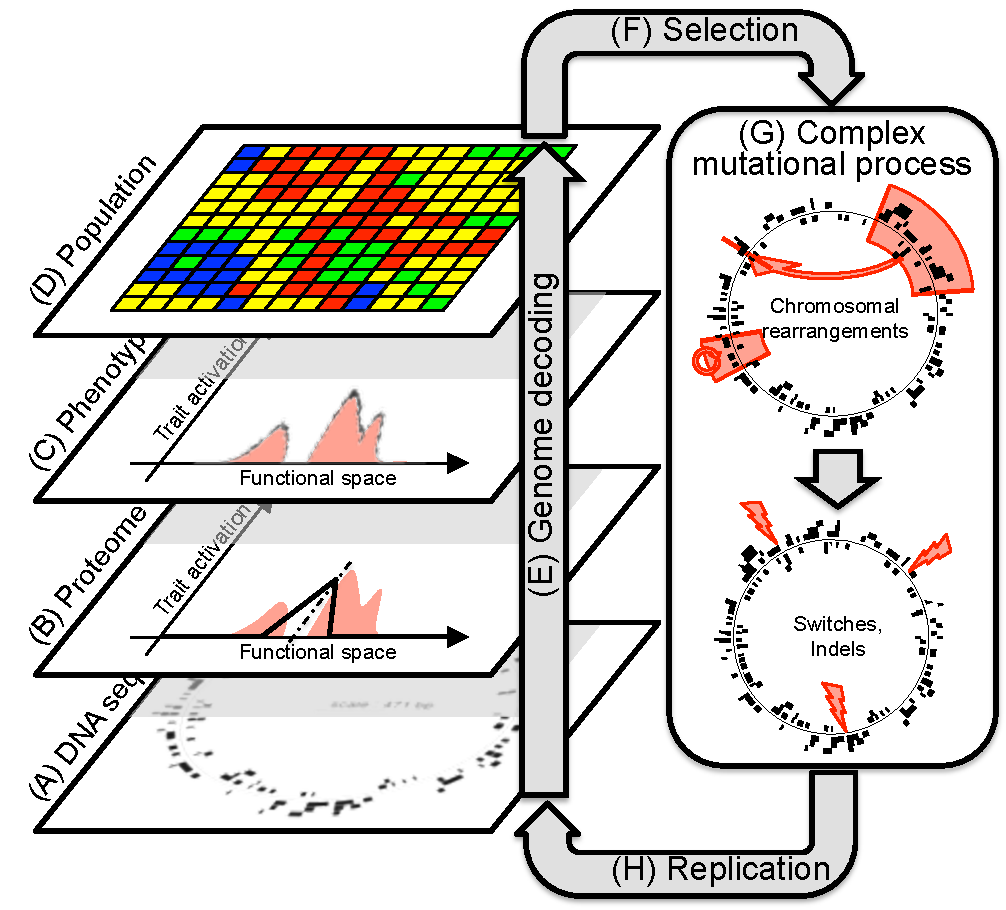
\includegraphics[width=\textwidth]{aevol/images/aevol.pdf}
\caption[Overview of the \emph{Aevol} model]{Broad overview of the \emph{Aevol} model.
In \emph{Aevol}, an evaluation-selection-replication evolutionary loop is applied to a population of individuals defined by their genome, encoded as a circular string of nucleotides (A, central ring), on which RNA sequences and genes are decoded (A, black segments).
The resulting proteins (B, in black) are mapped to an abstract phenotypic space, and summed in order to obtain the phenotype of the individual (C, in black), which is compared to an optimal phenotype (that implicitly represents the environment -- B and C, in pink), in order to compute its fitness.
In the model, the population is laid out on a square grid (D), with one individual per cell.
In order to produce a new generation, the ancestor of the new individual in each cell is chosen at random among the neighboring individuals, proportionally to their fitness (F).
Once this ancestor is chosen, its genome undergoes a series of random mutations, including rearrangements and local mutations (G), in order to obtain the genome of the new individual in the cell at the next generation (H).
}
\label{fig:aevol:model}
\end{figure}

\subsection{Overview}

The \emph{Aevol} platform, developed in the Inria Beagle team~\citep{rutten2019}, is a software suite designed to run artificial evolution experiments on a computer, rather than at the bench.
It was originally created to investigate the influence of classical population genetics parameters such as population size, mutation rate, or selection pressure on genomes themselves, seen as an integral part of the phenotype and not only as the source of genetic information.
In \emph{Aevol}, individuals have a very abstract phenotype, in exchange for a genome that is modeled down to the nucleotide level, and follows the ``central dogma of molecular biology''~\citep{crick1958}, with an accurate representation of RNA transcription and gene translation.
This approach contrasts with other artificial evolution platforms such as \emph{Avida}~\citep{adami1994,ofria2004}, which aim at studying the evolutionary process itself, rather than its impact on biological organisms.
For instance, \emph{Aevol} has been used to study the effect of mutation rate on genome size~\citep{knibbe2005}, or of the selection pressure on the percentage of non-coding bases and number of genes on the genome~\citep{batut2013}.
As an excellent and very thorough description of \emph{Aevol} (in French) can be found in~\cite{liard2020}, the following presentation of the model will be kept short and focused on the aspects relevant to this research.
Figure~\ref{fig:aevol:model} provides a comprehensive overview of the evolutionary algorithm at the core of \emph{Aevol}.

\subsection{The Genotype-Phenotype Map in \emph{Aevol}}

A genome or genotype in \emph{Aevol} consists in a sequence of binary characters ($0$ or $1$), which represents a double-stranded circular sequence of DNA.
The genome sequence explicitly describes the first (forward) strand of DNA, while the second (reverse) strand is obtained by complementing the sequence, replacing $0$ by $1$ and vice-versa.
In order to turn this genotype into a phenotype (Figure~\ref{fig:aevol:model} C), the decoding algorithm starts by looking for sequences that code for RNAs, reading the forward strand left-to-right and the reverse strand right-to-left.
An RNA starts with a promoter sequence, which has to match a consensus sequence with up to $d_{max}$ errors, and ends with a hairpin-like terminator.
Then, each RNA is scanned for genes, which start with a ribosome binding site followed by a 3-nucleotide start codon, which defines the reading frame.
Reading continues until a stop codon is found in the same frame, and the resulting string of codons is then translated into a protein, or discarded if no stop codon is found in frame before the end of the RNA sequence.
An RNA can thus contain zero, one, or several protein-coding genes.

As the genetic alphabet is binary in \emph{Aevol}, there are 8 different 3-nucleotide codons, and 6 codons can therefore be used to encode protein data, in addition to the start and stop codons.
These codons are grouped into three pairs, each respectively encoding the width $w$, height $h$, and mean position $m$ of a triangle kernel function from $[0, 1]$ to $[0, 1]$ (as represented in Figure~\ref{fig:aevol:model} B).
The mean $m$ represents the main function that the protein fulfills in the abstract phenotypic space, the height $h$ the intensity with which it does, and the width $w$ the pleiotropic ability of the protein to fulfill neighboring phenotypic functions.

In order to obtain the final contribution of the protein to the phenotype, the constitutive height $h$ of the gene is weighted by the expression level $e$ of the RNA that carries the gene, which depends on the activity of the promoter of that RNA.
In the model, the promoter activity decreases linearly with the difference $d$ between its sequence and the consensus sequence, and vanishes when $d > d_{max}$.
The expression level of the RNA is then given by the following equation: $e = 1 - \frac{d}{1+d_{max}}$.
Finally, in order to compute the complete phenotype of the individual from the set of its proteins, the kernel functions representing each gene are summed, resulting in a piecewise-linear phenotype function.
As the maximum degree to which each phenotypic function can be fulfilled is bounded by 1, the phenotype function is finally capped using Łukasiewicz operators in order to keep within this limit.

\subsection{Fitness}

Once the phenotype of an individual has been decoded from its genome, we can compute its fitness.
As the environment is indirectly specified by an optimal phenotype, we first compute a phenotypic gap as the integral of the absolute value of the difference between the phenotype of the individual and the optimal phenotype, taken over the range of phenotypic values (the $L^1$ distance between the functions).
Then, we compute the fitness as the inverse exponential of the phenotypic gap, multiplied by a selection coefficient: the higher the coefficient, the larger the difference in fitness between individuals with the same difference in gap.

\subsection{Mutational Operators}

Once the ancestor of a new individual has been chosen, a set of random mutations are applied to its genome to obtain the new genome.
These mutations are split into two classes, depending on the proportion of the genome that they can affect: genomic rearrangements, and local mutations.

Genomic rearrangements can affect up to the whole genome, and comprise four kinds of structural changes: duplications, deletions, inversions, and translocations.
In each of these rearrangements, the two endpoints of the affected segment are first drawn randomly on the genome.
In a large duplication, an additional insertion point is randomly selected on the genome, and the genetic content located between the endpoints is copied at the insertion point.
In a large deletion, the genetic content that was present between the endpoints is simply discarded.
In an inversion, the segment is reinserted left-to-right between the endpoints, reversing the orientation of every gene located on the inversion.
Finally, in a translocation, the genetic content is removed, turned into a circular plasmid, cut at a random point in the plasmid, and reinserted at another insertion point in the genome.

Local mutations, on the contrary, comprise small insertions, small deletions (collectively known as indels), and switches.
In a small insertion or deletion, up to 6 contiguous bases are either inserted (choosing each base at random) or deleted at a random point in the genome.
In a switch, the value of a random nucleotide is switched, from 1 to 0 or vice-versa.


\section{Modeling DNA Supercoiling in \emph{Aevol}}
\label{sec:aevol:aevol_sc}

In order to model the effect of supercoiling on gene transcription in \emph{Aevol}, I chose to start with very simple approximations,
concerning the level of supercoiling itself and its effect on transcription, as the \emph{Aevol} model is already quite complex on its own.

\begin{figure}
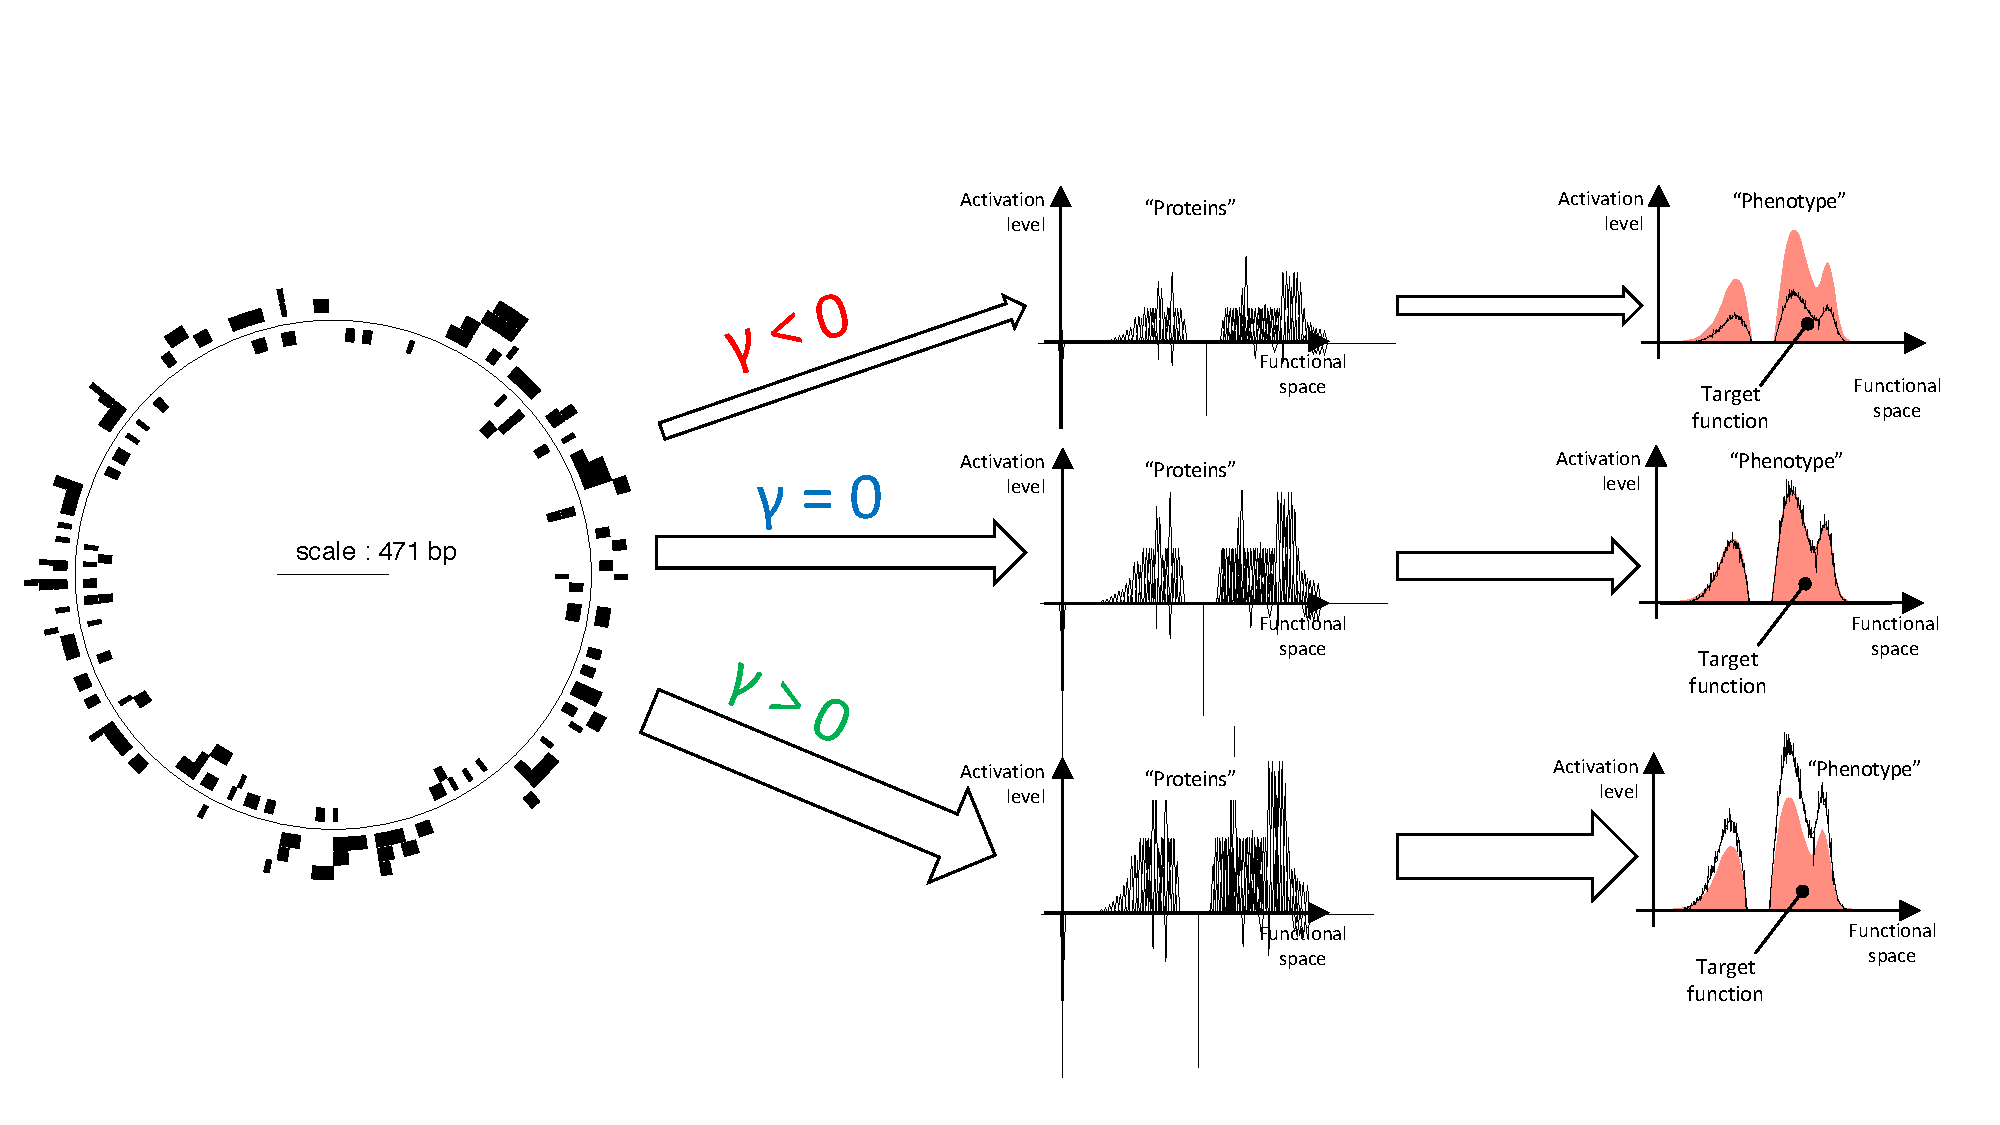
\includegraphics[width=\textwidth]{aevol/images/supercoiling_aevol.pdf}
\caption[Effect of supercoiling on the phenotype of an individual in \emph{Aevol}]{Effect of supercoiling on the phenotype of an \emph{Aevol} individual.
Left: genome (central ring) and genes (black rectangles) of the individual.
Middle: kernel function encoded by every gene in the phenotypic space, affected by an excess of positive supercoiling (top), no extra supercoiling (middle), or an excess of negative supercoiling (bottom).
Right: phenotype of the individual in each situation, compared to the optimal phenotype (in pink).}
\label{fig:aevol:sc_phenotype}
\end{figure}

\subsection{Level of DNA Supercoiling}
First, I consider the supercoiling level as constant along the genome and over time, which can be interpreted as taking the spatial and temporal average of the (actually dynamic) supercoiling level.
To implement this model inside \emph{Aevol}, I changed the genotype of individuals by adding, alongside the string-of-nucleotides genome, a single parameter $\gamma$ which represents the relative variation in the supercoiling level $\sigma$ of this individual compared to a reference supercoiling level $\sigma_0$: $\gamma = \frac{\sigma-\sigma_0}{\sigma_0}$.

\subsection{Gene Expression}
To keep the model as simple as possible, I also chose to model the effect of supercoiling on transcription as having the same linear effect on the transcription rate of every RNA on the genome.
I therefore updated the computation of the gene expression $e$ to take supercoiling into account, in addition to promoter activity:

\begin{equation}
e = (1 - \frac{d}{1+d_{max}}) \cdot (1 + \gamma)
\label{eq:aevol:sc}
\end{equation}

The effect of supercoiling on the phenotype of an example (pre-evolved) individual in the model is presented in Figure~\ref{fig:aevol:sc_phenotype}.
When $\gamma < 0$ (top row) -- when there is an excess of positive supercoiling compared to the baseline -- the expression of every gene is decreased.
When $\gamma$ is equal to 0 (middle row) -- when the supercoiling level is equal to the baseline -- there is no change to gene expression levels, which replicates the behavior of the original \emph{Aevol} model.
Finally, when $\gamma > 0$ (bottom row) -- when there is more negative supercoiling than in the baseline -- the expression of every gene is increased.

\subsection{Mutational Operator}
\label{sec:aevol:mut-sc}

In biological organisms, the supercoiling level is not only a direct property of the DNA molecule, but is also controlled by topoisomerases and nucleoid-associated proteins that are not modeled in \emph{Aevol} (as the phenotypic space is completely abstract), and changes in the supercoiling level come from mutations affecting the genes that encode these proteins, such as \emph{gyrA} or \emph{fis}~\citep{crozat2005}.
In order to model mutations in the supercoiling level in \emph{Aevol}, I chose a continuous model, in which a small variation in $\gamma$ indirectly reflects the effect of a mutation in one of the supercoiling-controlling genes.

When an individual reproduces, we first use a Bernoulli trial, with a probability $p$ that represents the probability that a supercoiling-protein gene undergoes a non-synonymous mutation, to decide whether to change the supercoiling level.
Then, if the supercoiling level should change, we draw a variation in relative supercoiling $\Delta\gamma$ according to a normal distribution $\mathcal{N}(0, s^2)$, and finally set the relative supercoiling level $\gamma'$ of the offspring to $\gamma' = \gamma + \Delta\gamma$.
The parameters of these laws are parameters of the simulation, and their values are given in Table~\ref{tab:aevol:param_values}.
Throughout this chapter, I will for the sake of clarity refer to the usual DNA-affecting mutations presented in~\ref{sec:aevol:model} as \emph{genomic mutations}, and to the mutations in the supercoiling level presented here as \emph{supercoiling mutations}.


\section{Results}
\label{sec:aevol:results}

As presented in the introduction of this chapter, the goal of implementing a supercoiling model in \emph{Aevol} was twofold.
The first aim was to see to which extent adding a new dimension to the phenotypic space, and a new mutational operator to explore this new dimension, would allow populations to evolve faster than allowed by the original model, thanks to the wide jumps in the phenotypic landscape that are made possible by the supercoiling mutations.
The second aim was to disentangle the possible epistatic effects between supercoiling mutations and genomic mutations in \emph{Aevol}.
In this section, I first present the experimental setup that I used in order to answer these questions.
Then, I show that adding regulation by supercoiling did not measurably increase the rate of adaptation of populations compared to the control, and that supercoiling indeed follows a very constrained evolutionary trajectory in these experiments.
Finally, I conclude that I could not find any observable epistasis between supercoiling and other mutations, when using the supercoiling model presented in Section~\ref{sec:aevol:model}.

\subsection{Experimental Setup}

In order to tackle these questions, I ran two sets of simulations: the experimental runs using the supercoiling model, and the control runs using the vanilla version of \emph{Aevol}.
Each set of runs comprises 5 replicate populations, which were evolved for 1,000,000 generations, each starting from a clonal population.
Each of the initial individuals was obtained by randomly drawing 5,000 bp-long genomes, until a genome with a non-zero fitness (i.e., at least one protein-coding gene partially matching the phenotypic target) was found.
The simulations were run on a 24-core Intel(R) Xeon(R) CPU E5-2620 v3 @ 2.40GHz server with 128 GB of RAM, and lasted approximately a week for each set of replicates.
The limited number of replicates for each set of simulations was chosen to balance their energy expenditure with the preliminary character of the work, which alleviates the need for statistical strength in the resulting data.
All the data from this experiment is available online on the \href{https://doi.org/10.5281/zenodo.7307545}{Zenodo} platform.

\subsection{Studying Lineages}

The data that is presented in the rest of this section was obtained by reconstructing the lineage, starting from the initial generation, of a random individual at the last generation of each replicate.
Studying a given lineage, rather than the best individual at every generation (which need not sire one another), allows us to reconstruct the precise set of mutations that happened throughout the evolutionary history of this lineage, and therefore gives us information about the possible causal link between these mutations, and hence about their possible epistatic relationships.

As a theoretical haploid Wright-Fisher population with $N$ individuals coalesces on average in $2N$ generations without mutation or selection~\citep{felsenstein2019}, we chose to analyze the data from generation 0 to 990,000 of every replicate (excluding the last 10,000 generations), ensuring that the last individual in each lineage is indeed ancestral to the whole population of the last generation of that replicate.

\begin{table}
\begin{center}
\begin{tabular}{ l r r }
\toprule
\textbf{Parameter} & \textbf{Symbol} & \textbf{Value}\\
\midrule
Population size & N & 1,024 (32x32 grid) \\
Initial genome size & $g_0$ & 5,000 bp \\
Local mutation rate & $\mu_{loc}$ & $10^{-7}$ bp$^{-1}$.gen$^{-1}$ \\
Rearrangement rate & $\mu_{rear}$ &$10^{-6}$ bp$^{-1}$.gen$^{-1}$ \\
\midrule
Initial supercoiling level & $\gamma_0$ & 0 \\
Supercoiling mutation probability & $p$ & $10^{-1}$ \\
Supercoiling mutation variance & $s^2$ & $10^{-2}$ \\
\midrule
Generations & T & 1,000,000 \\
Number of replicates & $n$ & 5\\
\bottomrule
\end{tabular}
\end{center}
\caption[Table of parameter values for the \emph{Aevol} runs]{Table of parameter values used in the \emph{Aevol} evolutionary runs.
The top part describes parameters common to the experimental and control set of rules, the middle part the supercoiling-related parameters introduced in the supercoiling model, and the bottom part simulation-specific parameters.}
\label{tab:aevol:param_values}
\end{table}


\subsection{Evolution of the Fitness Level}

\begin{figure}
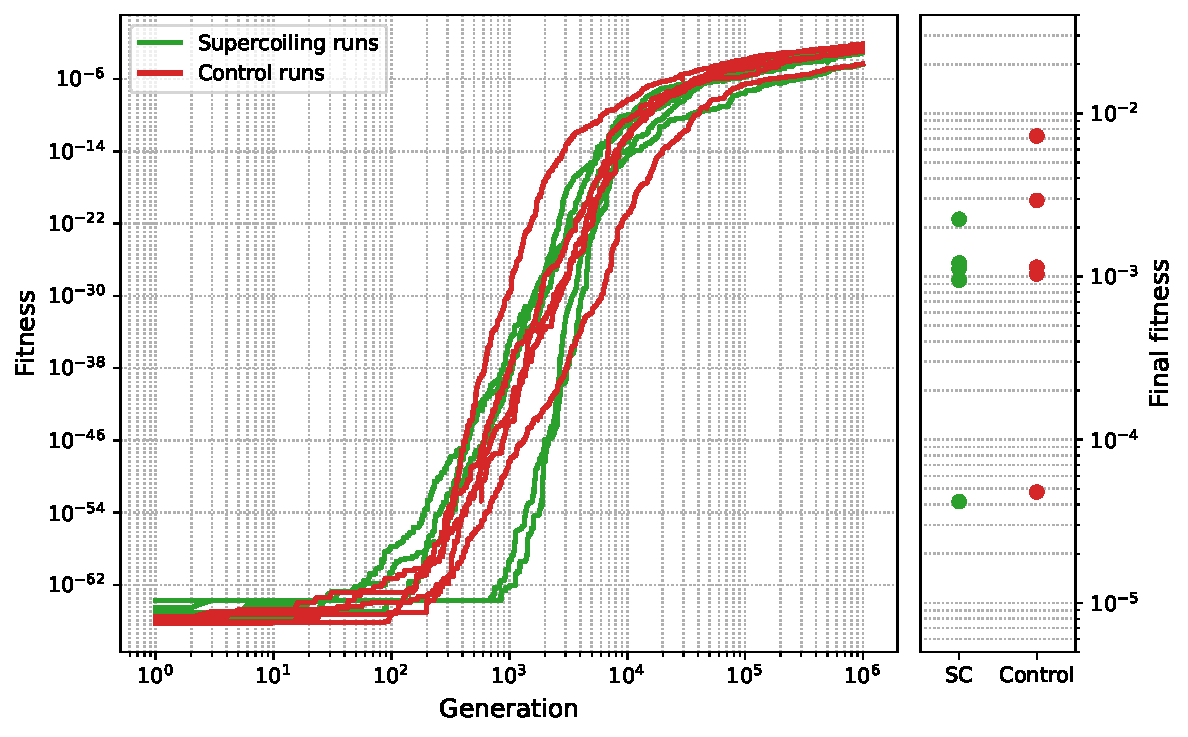
\includegraphics[width=\textwidth]{aevol/images/fitness_all.pdf}
\caption[Evolution of the fitness of the control and experimental runs in \emph{Aevol}]{Left: Evolution of the fitness at every generation throughout the lineage of the final population of each replicate of the experimental (green) and control (red) runs.
Both axes follow logarithmic scales.
Right: Fitness of the lineage individual at the 990,000th generation of each run, separated between supercoiling (green) and control (red) runs.}
\label{fig:aevol:fitness}
\end{figure}

Figure~\ref{fig:aevol:fitness} presents, on the left-hand side, the fitness of the individual at every generation of the lineage of the final population, or lineage individual, in each replicate.
In each case, fitness follows a broadly sigmoid shape (noting that both axes are logarithmic): the fitness of each run quickly increases from generation 100 up to generation 100,000, then slows down for the remaining 900,000 generations, but never completely ceases to progress, mirroring in \emph{Aevol} the open-ended evolution observed in the LTEE.
The right-hand side of Figure~\ref{fig:aevol:fitness} shows the fitness of the lineage individual at the 990,000th generation of each run.

With the limited number of replicates of each run, there is no discernible difference in fitness between the two experimental conditions, with and without mutations in the supercoiling level.
Adding the new phenotypic dimension of the supercoiling level, and the associated supercoiling mutational operator, therefore does not seem to play an important role in the rate of evolution of the populations modeled in \emph{Aevol}.

\subsection{Evolution of the Supercoiling Level}

\begin{figure}
\centering
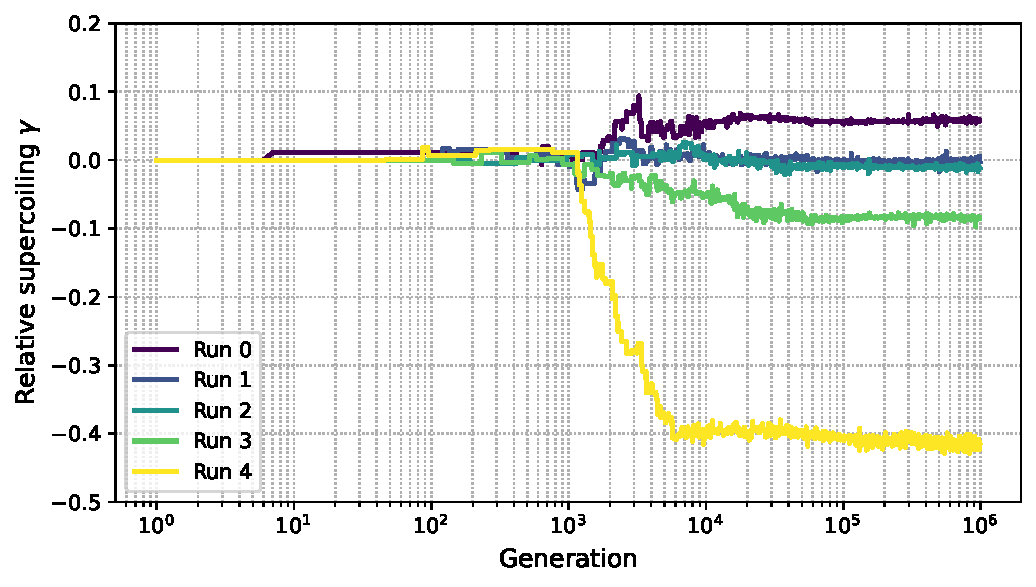
\includegraphics[width=0.9\textwidth]{aevol/images/supercoiling_all.pdf}
\caption[Evolution of the supercoiling level of the experimental runs in \emph{Aevol}]{Evolution of the relative level of supercoiling at every generation of the lineage of each of the experimental runs.}
\label{fig:aevol:sc}
\end{figure}

Figure~\ref{fig:aevol:sc} shows the evolution of the supercoiling level throughout the lineage in each of the 5 replicates.
In every run, the supercoiling level evolves only at the very beginning of the run, stabilizing in a few tens of thousands of generations, and remains essentially constant afterwards.
This is in strong contrast to the fitness of the runs (presented in Figure~\ref{fig:aevol:sc}), which keeps increasing until the end of the runs.

It therefore seems that the supercoiling level might play a role in the early evolution of the runs, but not in their long-term fitness improvement.
This result is in a sense slightly disappointing but was not entirely unexpected.
Indeed, in the early evolution of individuals in \emph{Aevol}, the phenotypic target is only very imperfectly approached by the proteins expressed by the individual.
At that stage, mutations in the supercoiling level, which affect the expression level of every protein equally, could indeed have a positive effect by bringing the whole phenotype closer to the optimum, in a very broad stroke.
Indeed, as individuals in \emph{Aevol} evolve from an ancestor with a single good gene, phenotypic functions are often under-performed by individuals at the early stages of evolution in the model, as the width and height of the kernel functions of their genes can be small, and as the expression level of their RNAs can be quite low if their promoters contain too many errors.
The different supercoiling values towards which each of the replicates tends to converge in Figure~\ref{fig:aevol:sc} could therefore be interpreted as a founding effect coming from the genome of the original individual in that run, which could be confirmed by a more detailed analysis of the series of mutations that happened in each lineage.

However, as evolution progresses, and as the optimal phenotype is more and more closely matched by the individual, changing the whole expression profile at once becomes less and less susceptible to be favorable.
This case is represented in Figure~\ref{fig:aevol:sc_phenotype}: any change in supercoiling, be it positive or negative, will decrease the fitness of the individual, and supercoiling mutations are therefore less and less susceptible to be picked up in the lineage.

These results tend to show that the model in which supercoiling has a global, linear effect on gene expression levels is too simplistic in order to produce phenotypic effects that are variable enough to have a chance to be picked up by selection; and therefore that this model is insufficient to study the interplay between supercoiling mutations and genomic mutations in \emph{Aevol}.

\subsection{Looking for Epistasis}

\paragraph{Waiting Intervals Before and After Mutations}
In order to detect signs of positive or negative epistasis between the different kinds of mutations, I used the following approach, which considers the waiting intervals before and after mutations happen: if, for a given mutation type, the average interval until a new favorable mutation fixes in the lineage after a mutation of that type is smaller than the average interval since the last favorable mutation before that mutation, this could be interpreted as a sign that the mutation has increased the probability of a favorable mutation happening; in other terms, as a broadening of the evolutionary paths available to the genome, or a sign of positive epistasis between that kind of mutation and other kinds of mutations.
On the contrary, if it takes longer for a new favorable mutation to fix in the lineage after that mutation, it would be a sign that the evolutionary paths have been constrained by the inversion: a sign of negative epistasis.

The data obtained following this approach is presented in Figure~\ref{fig:aevol:epistasis}.
For each mutation type, it shows the average number of mutations of that type that fixed in the lineage of each replicate, as well as the average time after which a mutation of that types fixes after a non-neutral mutation (left), and before a non-neutral mutation fixes after a mutation of that type (right), in the control runs (top) and in the experimental runs (bottom).

\paragraph{Epistasis of Duplications and Deletions}
In the control, a faint pattern seems to be discernible for large-scale inversions and deletions: the average time to a new mutation after a deletion is slightly higher than the time before a deletion, hinting that deletions could present a negative epistasis with other mutations.
Conversely, the time to a new mutation after a duplication is slightly lower than the time before the mutation, hinting that duplications could on the contrary present positive epistasis with other mutations.
Local mutations, as well as rearrangements and inversions, do however not seem to swing one way or the other.

In the experimental runs, no such pattern is visible at first sight, including for the supercoiling mutations, and the global average waiting intervals are smaller than in the control, which is consistent with the introduction of a new mutation type.
There therefore seems to be no sign of epistasis between supercoiling mutations and genomic mutations, when following the approach explained above.

\begin{figure}
\centering
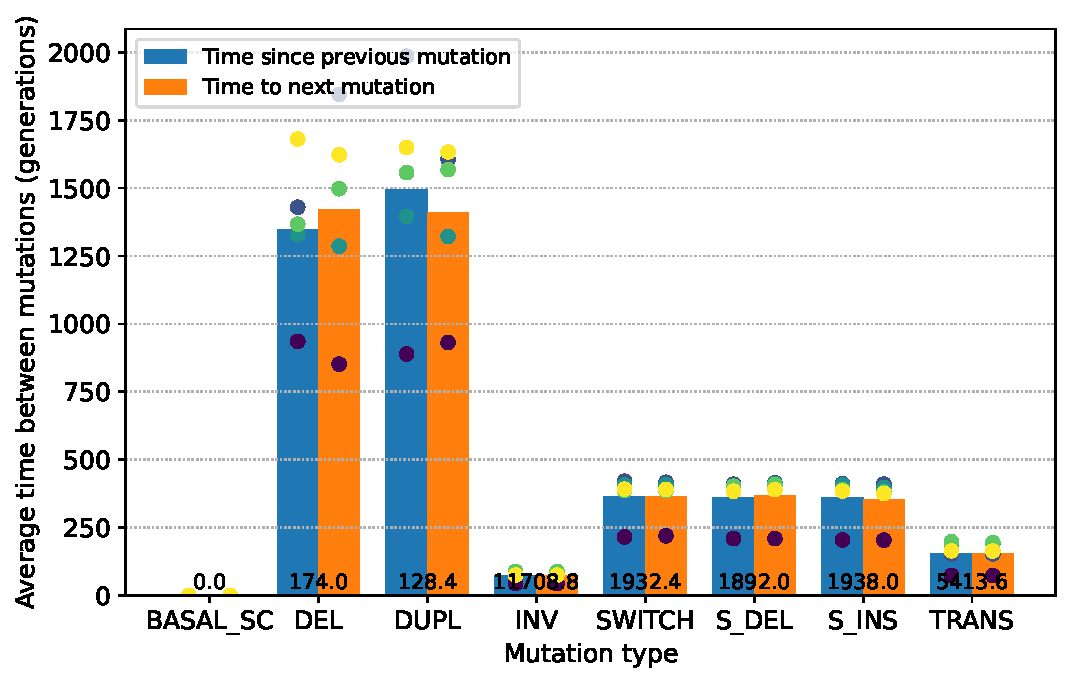
\includegraphics[width=0.9\textwidth]{aevol/images/epistasis_control.pdf}
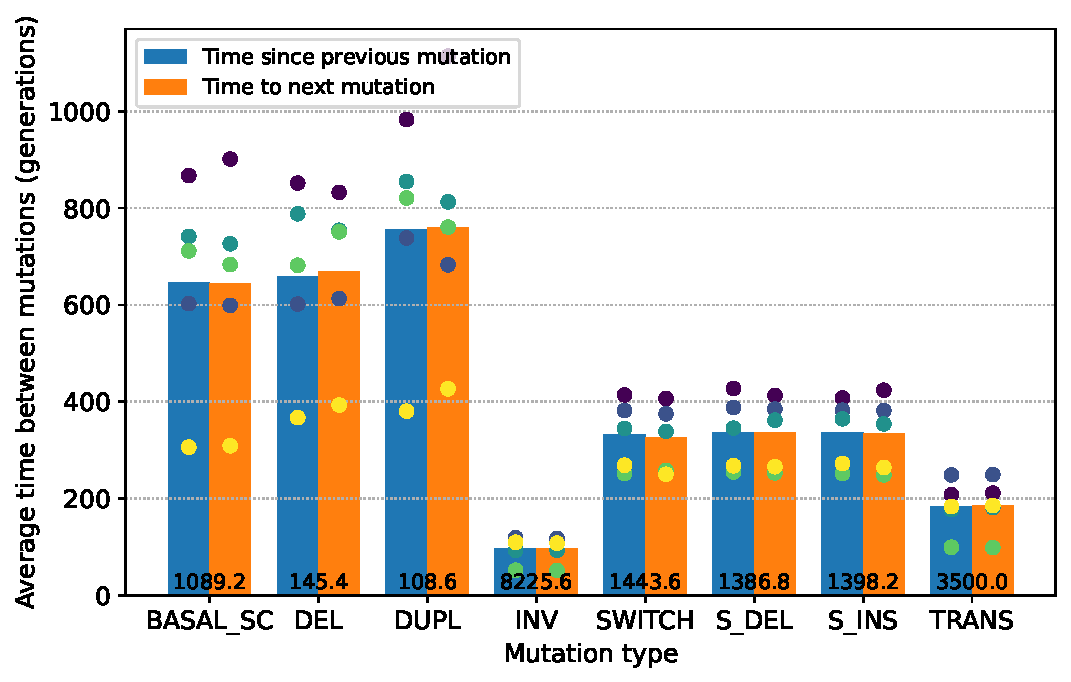
\includegraphics[width=0.9\textwidth]{aevol/images/epistasis_sc.pdf}
\caption[Measuring epistasis with the average times before and after mutations]{Average time before and after a mutation of each kind, in the control runs (top) and the experimental runs (bottom).
For each kind of mutation, the times presented show the wait time until a neutral mutation of that kind after a non-neutral mutation of any kind, and the time until the next non-neutral mutation of any kind after a mutation of that kind.
The bars show the average over the five replicates, and the colored dots show the value for every replicate.
The average number of neutral mutations of each type is displayed at the bottom of the corresponding bar.}
\label{fig:aevol:epistasis}
\end{figure}

\paragraph{Role of the Genome Size}
A hypothesis that could explain the pattern visible in the control runs for large deletions and duplications is that the difference in waiting intervals -- positive or negative epistasis -- is simply due to the change in the genome size caused by these mutations.
All mutation rates in the model are indeed proportional to the genome size, and the expected number of mutations at each generation therefore increases and decreases with the genome size (assuming that there is no fitness effect or selection).
However, in the experimental runs, the probability of a supercoiling mutation does importantly not depend on the genome size.
A hypothesis to explain the disappearance of the signal (possibly) there in the control for duplications and deletions could therefore be that supercoiling mutations tick according to their own clock, which depends on their parameters $p$ and $s^2$, but not on the state of the genome itself.
For example, if a certain beneficial indel is allowed to happen because of a duplication and indeed happens sometime after that duplication in the lineage, but a supercoiling mutation has happened between the duplication and the indel, then the signal from this particular epistatic relationship will have been hidden by that supercoiling mutation.

\section{Conclusion}
\label{sec:aevol:ccl}

The goal of this initial work was to study how supercoiling mutations affect the fitness landscape of individuals in \emph{Aevol}, that is the possible epistatic interactions between supercoiling mutations and other kinds of mutations.
In order to tackle this question, I implemented a model of the effect of the supercoiling level on gene expression, as well as a model of mutations in the supercoiling level, in \emph{Aevol}.
Using this version of the model, I ran evolutionary experiments, in which I compared the evolution of populations with supercoiling with control populations by analyzing the fitness, supercoiling level, and mutations fixed in the lineage of individuals that leads to the final population of every replicate.

With the limited data that was available, I could not find a difference in the evolution rates of each set of experiments, and deduced that supercoiling does not seem to play an important evolutionary role in this model; this result was substantiated by the fact that the supercoiling level converges very quickly to a fixed level in the evolutionary history of each population.
I then tried to detect signals of positive or negative epistasis between the different kinds of mutations, by looking at the waiting intervals between each kind of mutation.
While this approach did not lead to meaningful results in the experimental runs, it did hint at a possible epistatic link between duplications or deletions and the other mutation kinds, due to their effect on genome size, in the control runs, which seems promising for further investigation.

\paragraph{}
The verdict of these preliminary experiments was that the model of supercoiling that I implemented in \emph{Aevol}, in which supercoiling is kept constant along the genome and affects the expression level of all genes equally, was probably too simplistic to obtain meaningful results.
Rather than pursuing this avenue of research further by implementing a more precise model in \emph{Aevol}, I chose instead to go in a different direction.
In order to decouple the complexity of the \emph{Aevol} model from the study of the evolutionary role of supercoiling, I decided to simplify the individual model, genotype-phenotype map, and mutational operators as much as possible, in order to model the effect of supercoiling on gene expression more precisely while keeping the overall complexity of the model in check.
The results of this renewed approach are presented in the following chapters.
\chapter{Evolution of Environmental Sensing through DNA Supercoiling}
\chaptermark{Evolution of Environmental Sensing through DNA SC}
\label{chap:alife}

This chapter presents the proof-of-concept version of the \emph{EvoTSC} model, and the first results that I obtained with that version of the model: I show that the evolution of differentiated expression levels in different environments is possible when gene expression is only regulated by the transcription-supercoiling coupling.
The text of the chapter is an edited version of an article published in the \emph{Artificial Life} journal~\citep{grohens2022a}.

\paragraph{}
Both the importance of gene regulation via supercoiling and the detailed mechanisms of the transcription"=supercoiling coupling, at the local scale, have already been studied extensively in the literature (see Section~\ref{sec:background:sc}).
However, a thorough analysis of the effect of the transcription-supercoiling coupling on gene expression at the whole-genome scale -- and of its possible evolutionary use by natural selection -- remains lacking, in particular in the dense prokaryotic genomes, in which large groups of genes are likely to interact through this coupling.
In this work, we describe a new model which incorporates a high-level model of global supercoiling regulation and of the transcription"=supercoiling coupling within an \emph{in silico} experimental evolution setting.
Using this model, we first investigate the non-linear variation in gene transcription levels at the whole-genome scale in response to variations in the global supercoiling level.
Then, we study the evolutionary trajectory of gene activation patterns in individuals subjected to different environments.

We show that in our model, a genome-scale gene interaction network emerges from local supercoiling-mediated interactions, and creates a reaction norm in response to the change of a single parameter, the global supercoiling level, caused by different environments.
Moreover, we demonstrate that, using genomic inversions as the only mutation operator, and therefore only changing the relative positions and orientations of genes on the genome, evolution can select genomes displaying qualitatively different phenotypes in different environments characterized by different global supercoiling conditions.

%This article is an extended version of~\cite{grohens2021}.

\section{A Genome-Wide Model of the Transcription-Supercoiling Coupling}
\label{sec:alife:indiv_model}

\begin{figure}[H]
\centering
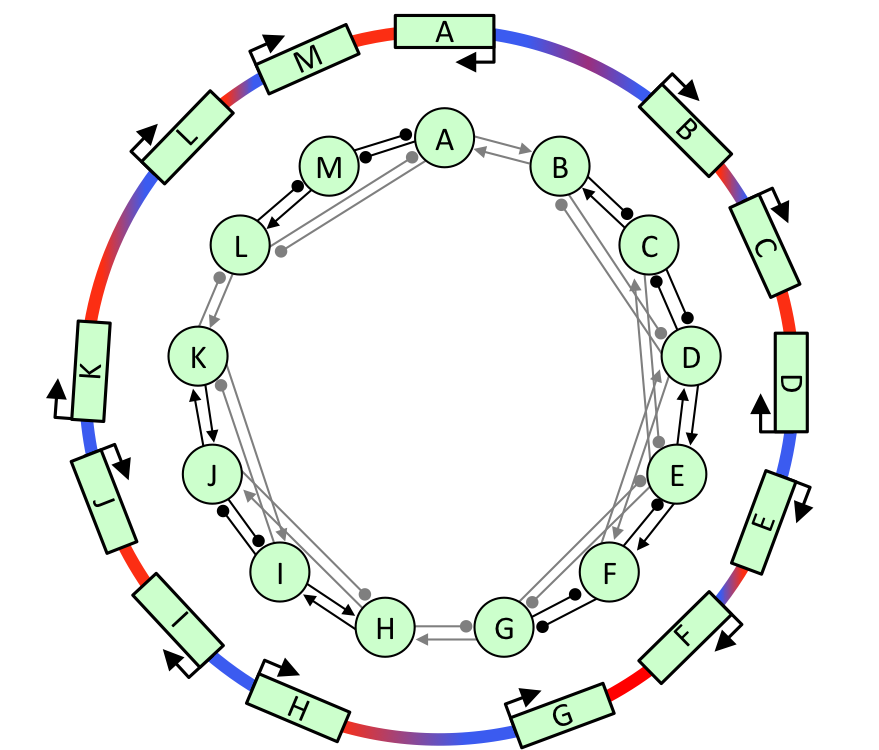
\includegraphics[width=0.75\textwidth]{alife/img/reseau.png}
\caption[Hand-drawn genome and local interactions resulting from the TSC]{Genes along an example genome and local variations in supercoiling (outer ring), and the associated gene interaction network (inner ring).
The outer ring color shows locally high ($\sigma > \sigma_0$, red) or low ($\sigma < \sigma_0$, blue) supercoiling levels due to gene transcription.
In the inner ring, closer genes interact more strongly (black arrows) than genes that are farther apart (gray arrows), either positively or negatively depending on their relative orientations.}
\label{fig:alife:network}
\end{figure}

%In this paper, we present a model which aims at studying the genome-wide effect of the transcription-supercoiling coupling in bacteria, expanding upon previous work which only considered local interactions.
%In gene-dense genomes such as prokaryotic ones, transcription-supercoiling coupling between nearby genes is likely to give rise to a genome-wide transcriptional network, the topology of which depends on relative gene distances and orientations.

Our model consists in an individual-based simulation, written in Python.
Its source code is available at \url{https://gitlab.inria.fr/tgrohens/evotsc/-/tree/alife-journal}.
It is also preserved for \href{https://archive.softwareheritage.org/swh:1:rev:6fc36abc1661c295782886647c37ef05ffb9d357}{long-term archival} using the Software Heritage online archive~\citep{dicosmo2020}.
An individual in the model is represented by a circular genome (representative of most bacterial genomes), comprising a fixed number of genes, separated by non-coding intergenic regions.
Each gene is described by the following characteristics: its locus on the genome, its orientation, and its basal transcription (or expression) level.
As we are mainly interested in the interplay between supercoiling and transcription, we voluntarily do not make the difference between gene expression levels, understood as mRNA or protein concentrations, and transcription levels, the immediate rate of mRNA
production.
Indeed, assuming a separation of timescales between the fast equilibrium of the transcription-supercoiling coupling, and the slow degradation of mRNAs, the concentration of a given mRNA is directly proportional to the transcription rate of its source gene.

Figure~\ref{fig:alife:network} illustrates the role played by the transcription-supercoiling coupling in an example genome.
It includes the local supercoiling variations due to gene transcription, and the resulting gene interaction network, with each gene possibly activating or inhibiting its neighbors, depending on their relative orientations.
Importantly to our approach, here genes do not interact only with their closest neighbors, but also with more distant genes, as is likely to be the case in the gene-rich bacterial genomes: \emph{E. coli} gene promoters are around one thousand base pairs apart~\citep{peter2004}, and the transcription-generated supercoiling propagates around a few thousand base pairs on each side of the transcription site~\citep{postow2004}.


\subsection{Mathematical Description of the Model}

We model the transcription-supercoiling coupling between an individual's genes as a system of equations, which relate the supercoiling level at the locus of each gene $\sigma_i$ (for $i$ ranging from $1$ to $n$, the number of genes of the individual), and the expression level of every gene $e_i$.
The parameters of the system are described by the genome of the individual, as will be detailed below.

In our model, the supercoiling at a given locus on the genome depends on three factors: the individual's basal supercoiling level $\sigma_{basal}$, the variation in supercoiling due to environmental conditions $\sigma_{env}$, and the variation in supercoiling due to the transcription of the neighboring genes.
We compute this local variation in supercoiling at the locus of each gene with the help of a gene interaction matrix, whose coefficient at position $(i, j)$ describes the influence of gene $j$ on gene $i$.
The coefficients are given by the following equation:

\begin{equation}
\frac{\partial\sigma_{i}}{\partial e_j} = \eta\cdot c \cdot\max(1-\frac{d(i, j)}{d_{max}}, 0)
\label{eq:dsde}
\end{equation}
%This interaction level abstracts the influence of local supercoiling into a single value, which reflects the positive or negative influence of each gene on the transcription level of the other genes in the genome.

More precisely, the interaction level between two genes depends on the relative orientation of the genes, as the transcription of a gene increases supercoiling at the locus of downstream genes and decreases supercoiling at the locus of upstream genes (remember that an increase in supercoiling means a decrease in transcription).
Therefore, we choose $\eta = 1$ if gene $i$ is downstream of gene $j$ and $\eta = -1$ otherwise (if $i=j$, $\eta = 0$ as a gene does not interact with itself).
The interaction level also depends on gene distance, as genes that are further apart on the genome interact less strongly, so the strength of the interaction linearly decreases with the intergenic distance $d(i, j)$, and reaches 0 when $d(i, j) = d_{max}$, the maximum distance above which the interaction vanishes.
Finally, an interaction coefficient $c$ is applied to adjust the strength of the coupling.

Using this interaction matrix, we compute the level of supercoiling $\sigma_i$ at the locus of every gene, which depends on the transcription level of all the other genes, on the basal supercoiling level, and on the environmental supercoiling level:

\begin{equation}
\sigma_i = \sigma_{basal} + \sigma_{env} + \sum_{j=1}^n\frac{\partial\sigma_{i}}{\partial e_j}e_j
\label{eq:alife_sigma}
\end{equation}

The transcription level $e_i$ of every gene as a function of total supercoiling is then modeled with a sigmoidal activation curve, following~\cite{elhoudaigui2019}.
The equation is given below:

\begin{equation}
e_i = \frac{1}{1 + e^{(\sigma_i - \sigma_0)/\epsilon}}
\label{eq:transcr}
\end{equation}

In this equation, $\sigma_0$ is a parameter that represents the inflexion point of the sigmoid, that is the supercoiling level at which the gene is at half its maximum transcription rate, and $\epsilon$ a scaling factor that represents the strength of the dependence of the transcription level on the supercoiling level.

Finally, in order to obtain the phenotype of an individual, we numerically compute a solution to the system of equations~\ref{eq:alife_sigma} and~\ref{eq:transcr}, using a fixed point algorithm.
This solution represents the state (of gene expression and supercoiling at every locus) towards which the individual would converge over time.
Let $f(e_i)$ be the function that computes new supercoiling levels $\sigma'_i$ from $e_i$ using equation~\ref{eq:alife_sigma}, and then computes new expression levels $e'_i$ from the new $\sigma'_i$ using equation~\ref{eq:transcr}, and finally returns $e'_i$.
In order to compute a fixed point of $f$, that is a set of transcription levels $e_i^*$ such that $f(e_i^*) = e_i^*$, we start with basal transcription levels $e_i^0$ (that are a property of each gene), and iterate the sequence $e_i^{t+1} = \frac{1}{2}(e_i^t + f(e_i^t))$, until the difference between two successive iterations is below a given threshold.
In our setting, this algorithm has empirically always converged to a solution that is a stable fixed point of the function, and that is therefore interpretable from a biological perspective.

\begin{figure}[H]
\centering
\begin{subfigure}[t]{0.42\textwidth}
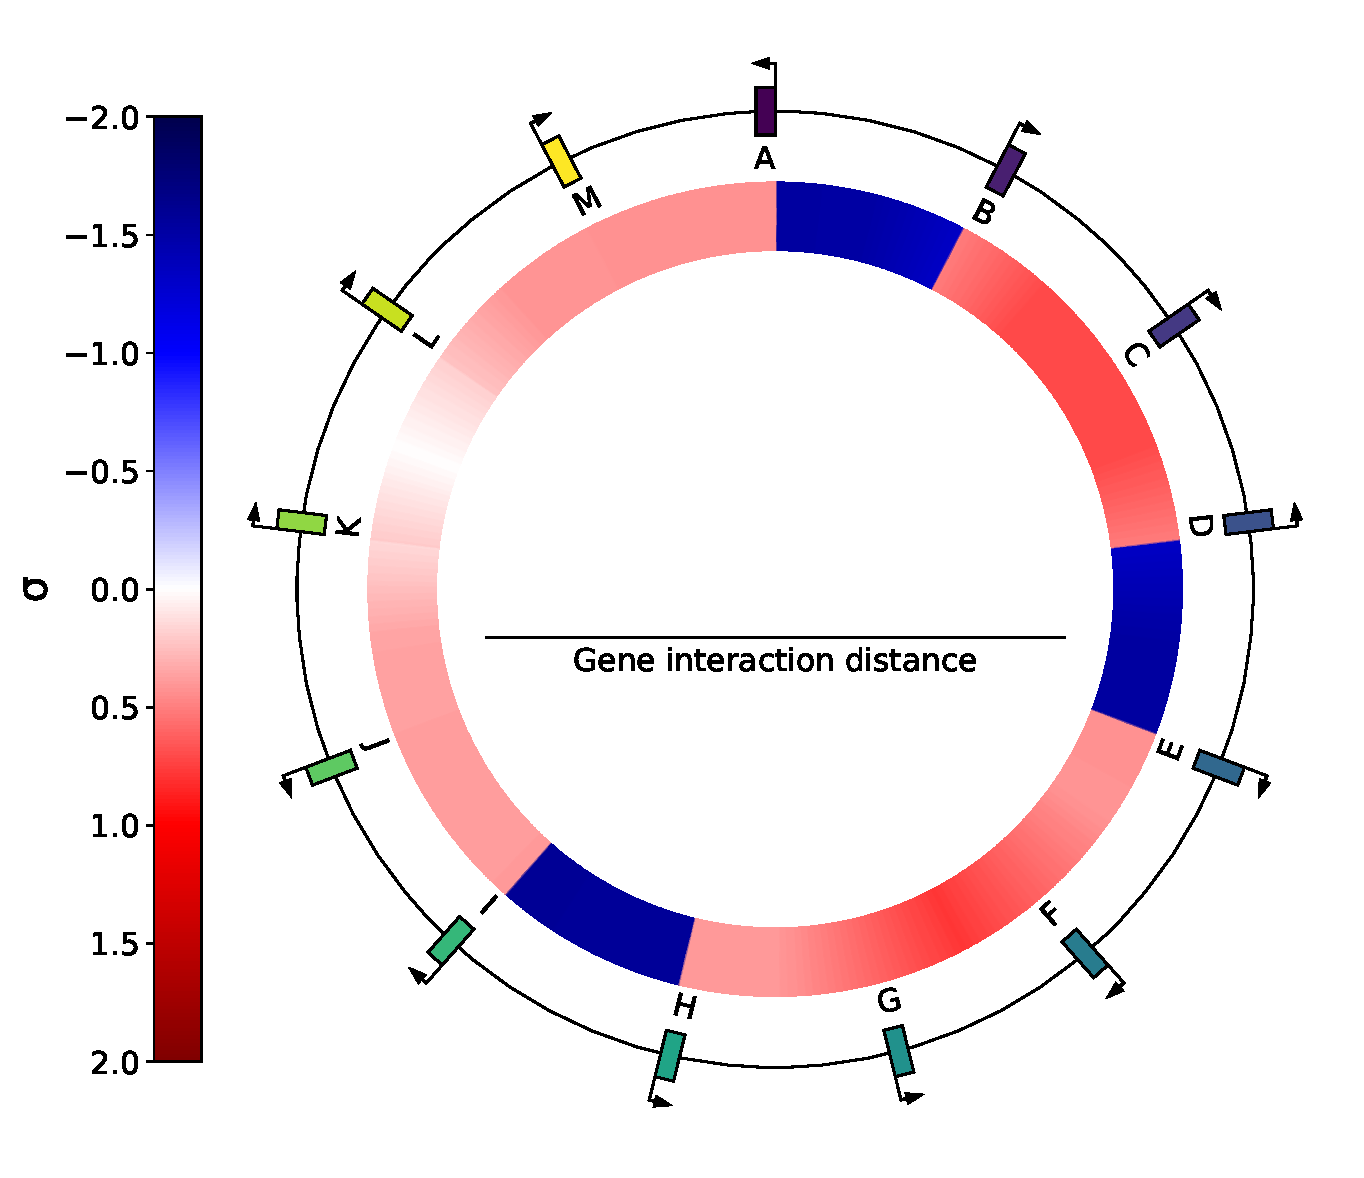
\includegraphics[width=\textwidth]{alife/img/13genes_genome.pdf}
\label{subfig:alife:13genes_genome}
\end{subfigure}
\begin{subfigure}[t]{0.56\textwidth}
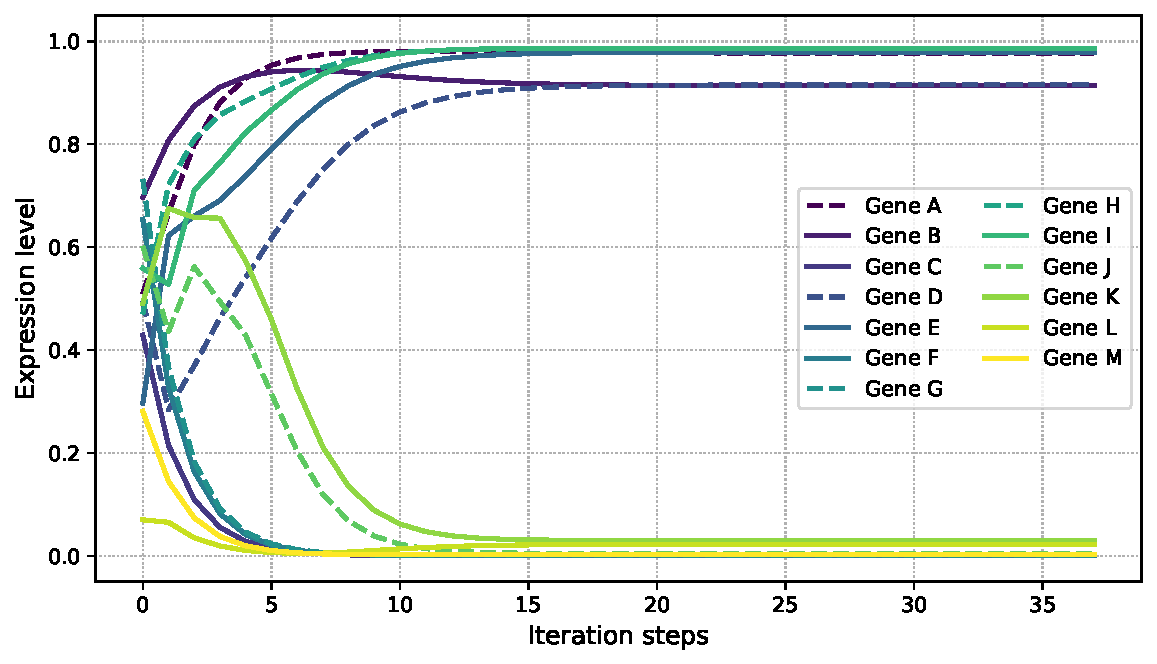
\includegraphics[width=\textwidth]{alife/img/13genes_expr_level.pdf}
\label{subfig:alife:13genes_expr}
\end{subfigure}
\caption[Example individual in the proof-of-concept model]{Left: genome (outer ring) and stable state level of supercoiling $\sigma$ (inner ring) of an example individual with 13 genes in the model.
Right: transcription levels of the individual's genes during the iterations of the fixed point computation, in an environment given by $\sigma_{env} = 0.05$.
Solid lines represent genes in forward orientation, and dashed lines represent genes in reverse orientation.}
\label{fig:alife:13genes}
\end{figure}

Figure~\ref{fig:alife:13genes} shows the genome (left, outer ring) of an example individual with a genome of 13,000 bp and $n=13$ genes evenly spaced along the genome, and with a basal supercoiling of $\sigma_{basal} = -0.06$.
The basal transcription level of each gene is randomly chosen between 0 and 1, and all the iterations of the fixed point algorithm that result in the final gene transcription levels are shown on the right.
In this individual, the non-linear effect of the interaction between neighboring genes is clearly visible.
Indeed, six genes (A, B, D, E, H, and I) end up at a high transcription rate at the fixed point (or solution) of the system, while the others end up at low transcription rates.
These activated genes can be grouped into 3 pairs (A and B, D and E, H and I), all of which are pairs of adjacent genes in divergent orientations.
Even though gene D has a low (around 0.3) basal transcription rate, it eventually reaches a high transcription state because of its positive interaction with gene E.
Conversely, genes F and G start with a high transcription rate, but are repressed by their neighbors H and E, and are therefore silenced as the system converges.
We can also observe complex behaviors in the model, as the gene expression levels pass through very different states during convergence to the solution.
Indeed, the transcription level of gene K initially increases due to its interaction with gene J, but both genes end up in a low transcription state, as they are inhibited by the very active gene I.
The final supercoiling level along the genome (left, inner ring) moreover demonstrates the effect of the transcription-supercoiling coupling on local supercoiling.
Highly transcribed genes, such as A and B, generate a large variation in the supercoiling level on their upstream and downstream sides, and the positive feedback loop between genes in divergent pairs is made clear by the very high negative value of the supercoiling level between each of the genes in these two pairs.


\subsection{Effect of the Environmental Supercoiling on Gene Activation Levels}
\label{sec:alife:env_model}

\begin{figure}[H]
\centering
\begin{subfigure}[t]{0.28\textwidth}
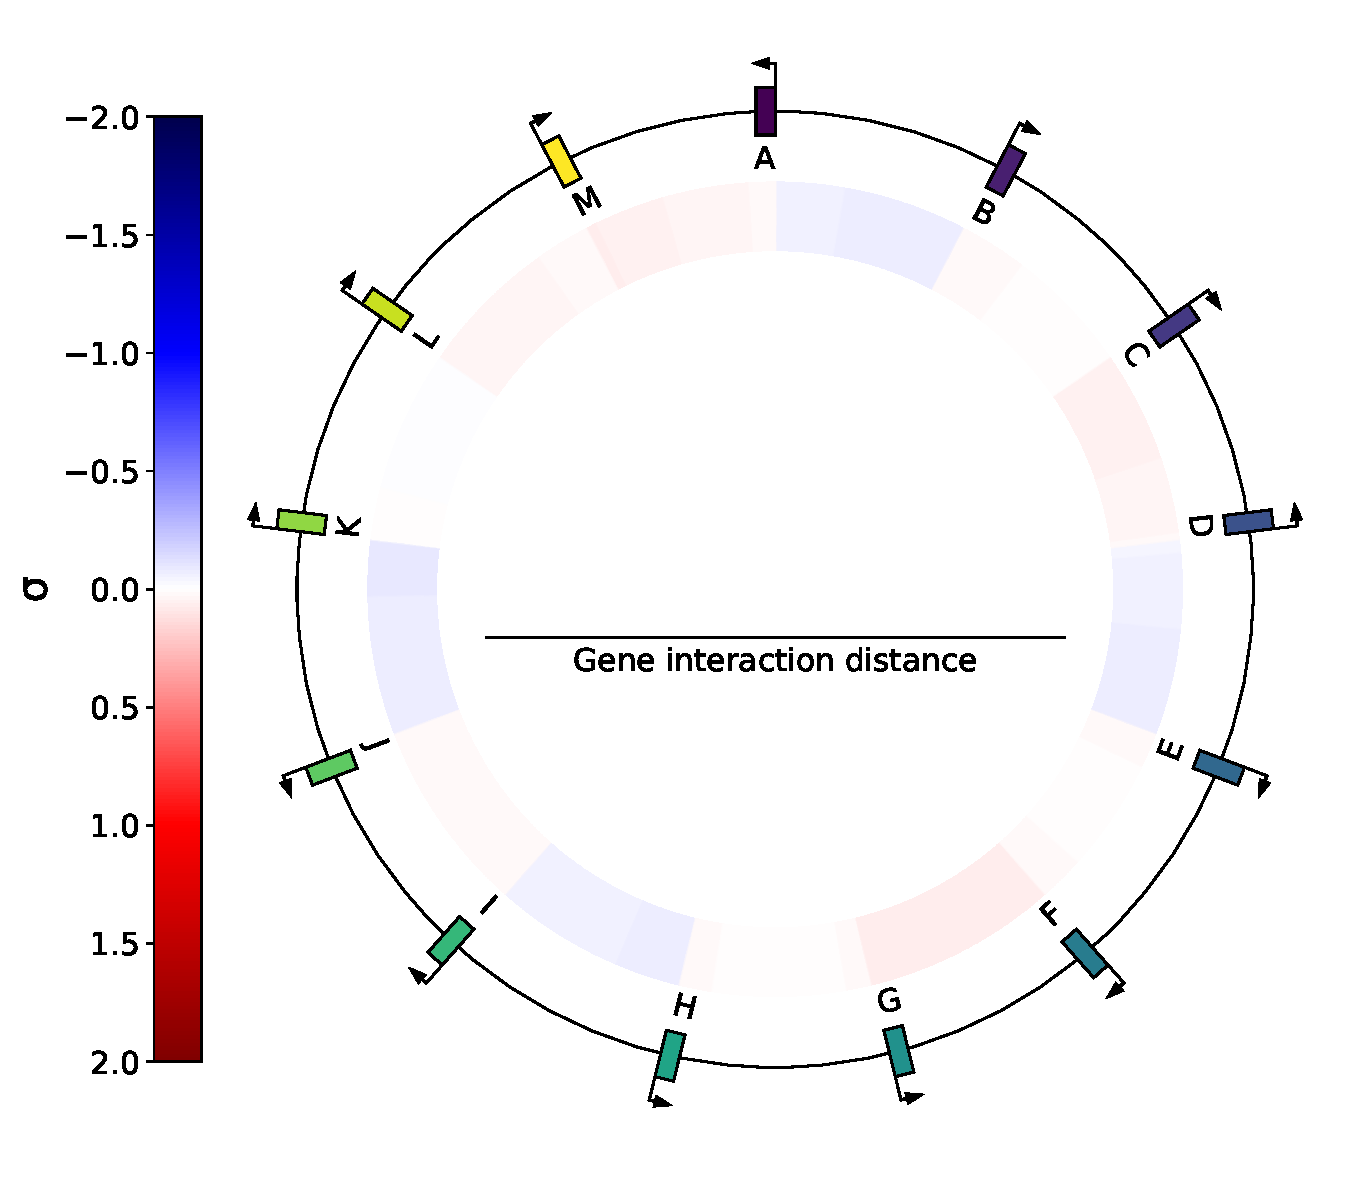
\includegraphics[width=\textwidth]{alife/img/13genes_genome_3.pdf}
\label{subfig:alife:genome_3}
\end{subfigure}
\hspace{-3mm}
\begin{subfigure}[t]{0.24\textwidth}
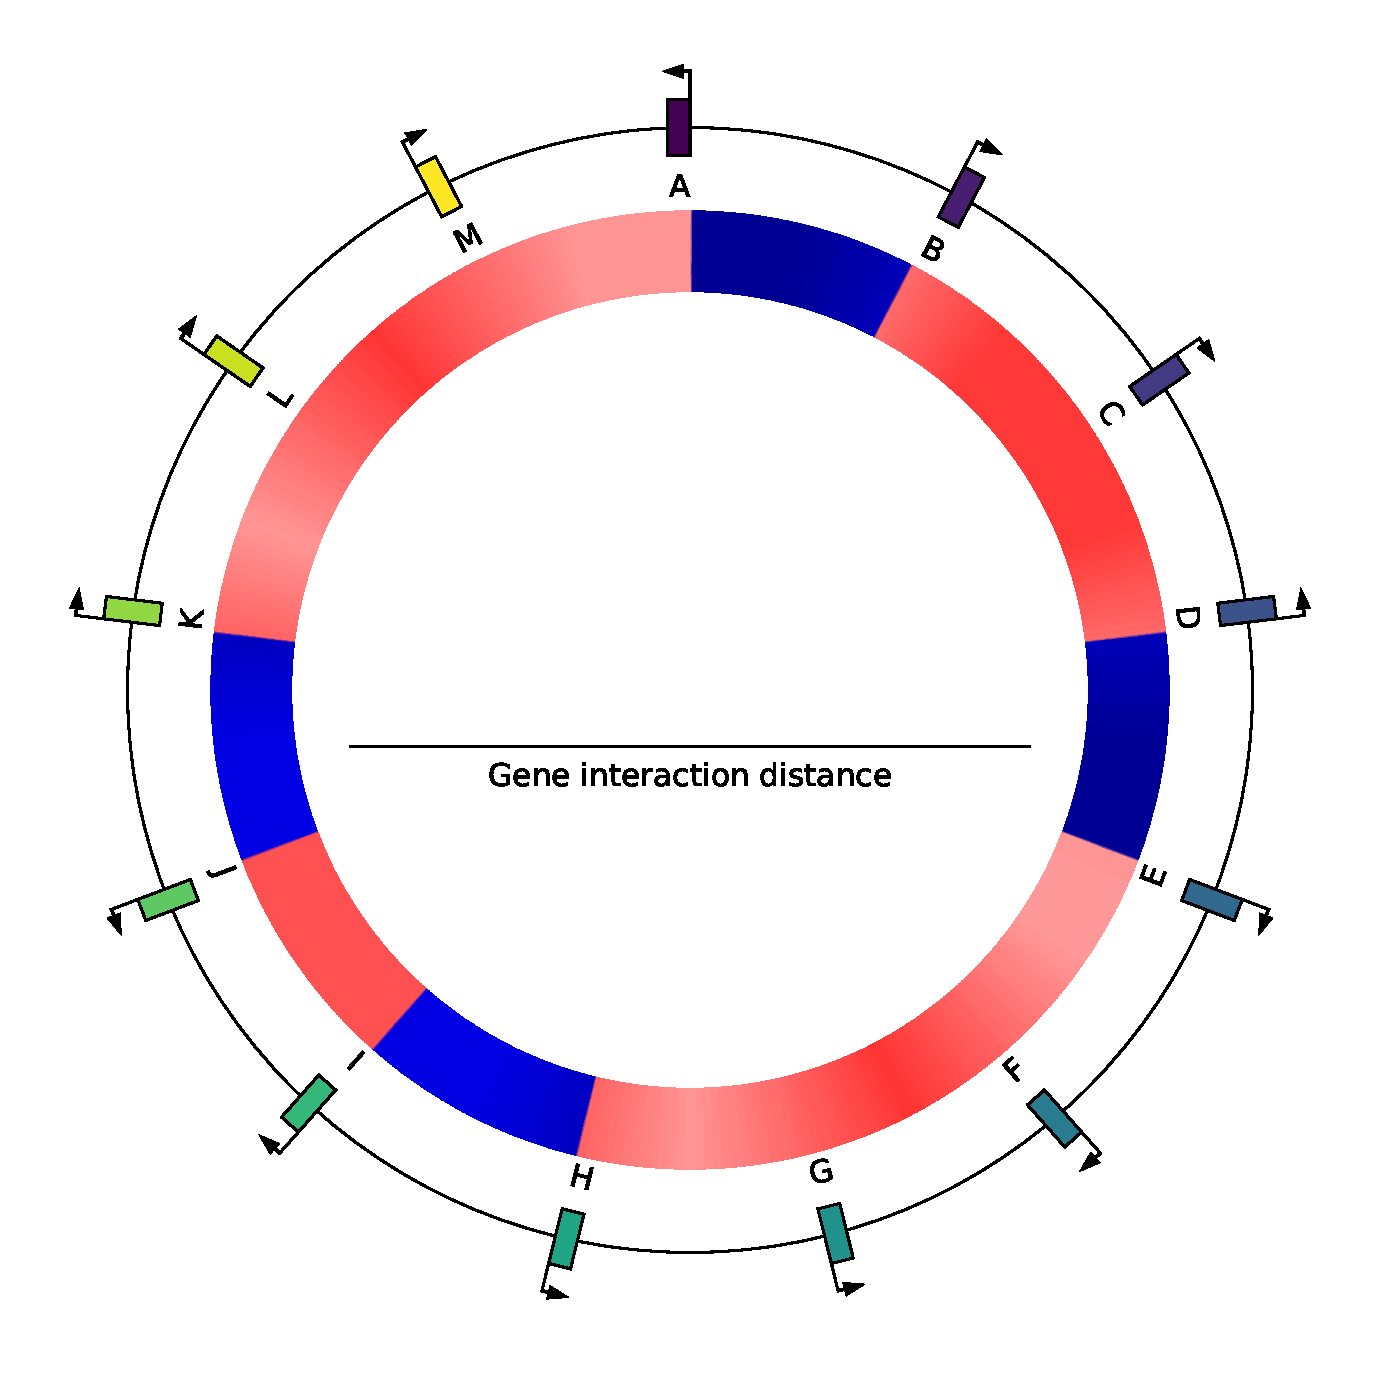
\includegraphics[width=\textwidth]{alife/img/13genes_genome_2.pdf}
\label{subfig:alife:genome_2}
\end{subfigure}
\hspace{-3mm}
\begin{subfigure}[t]{0.24\textwidth}
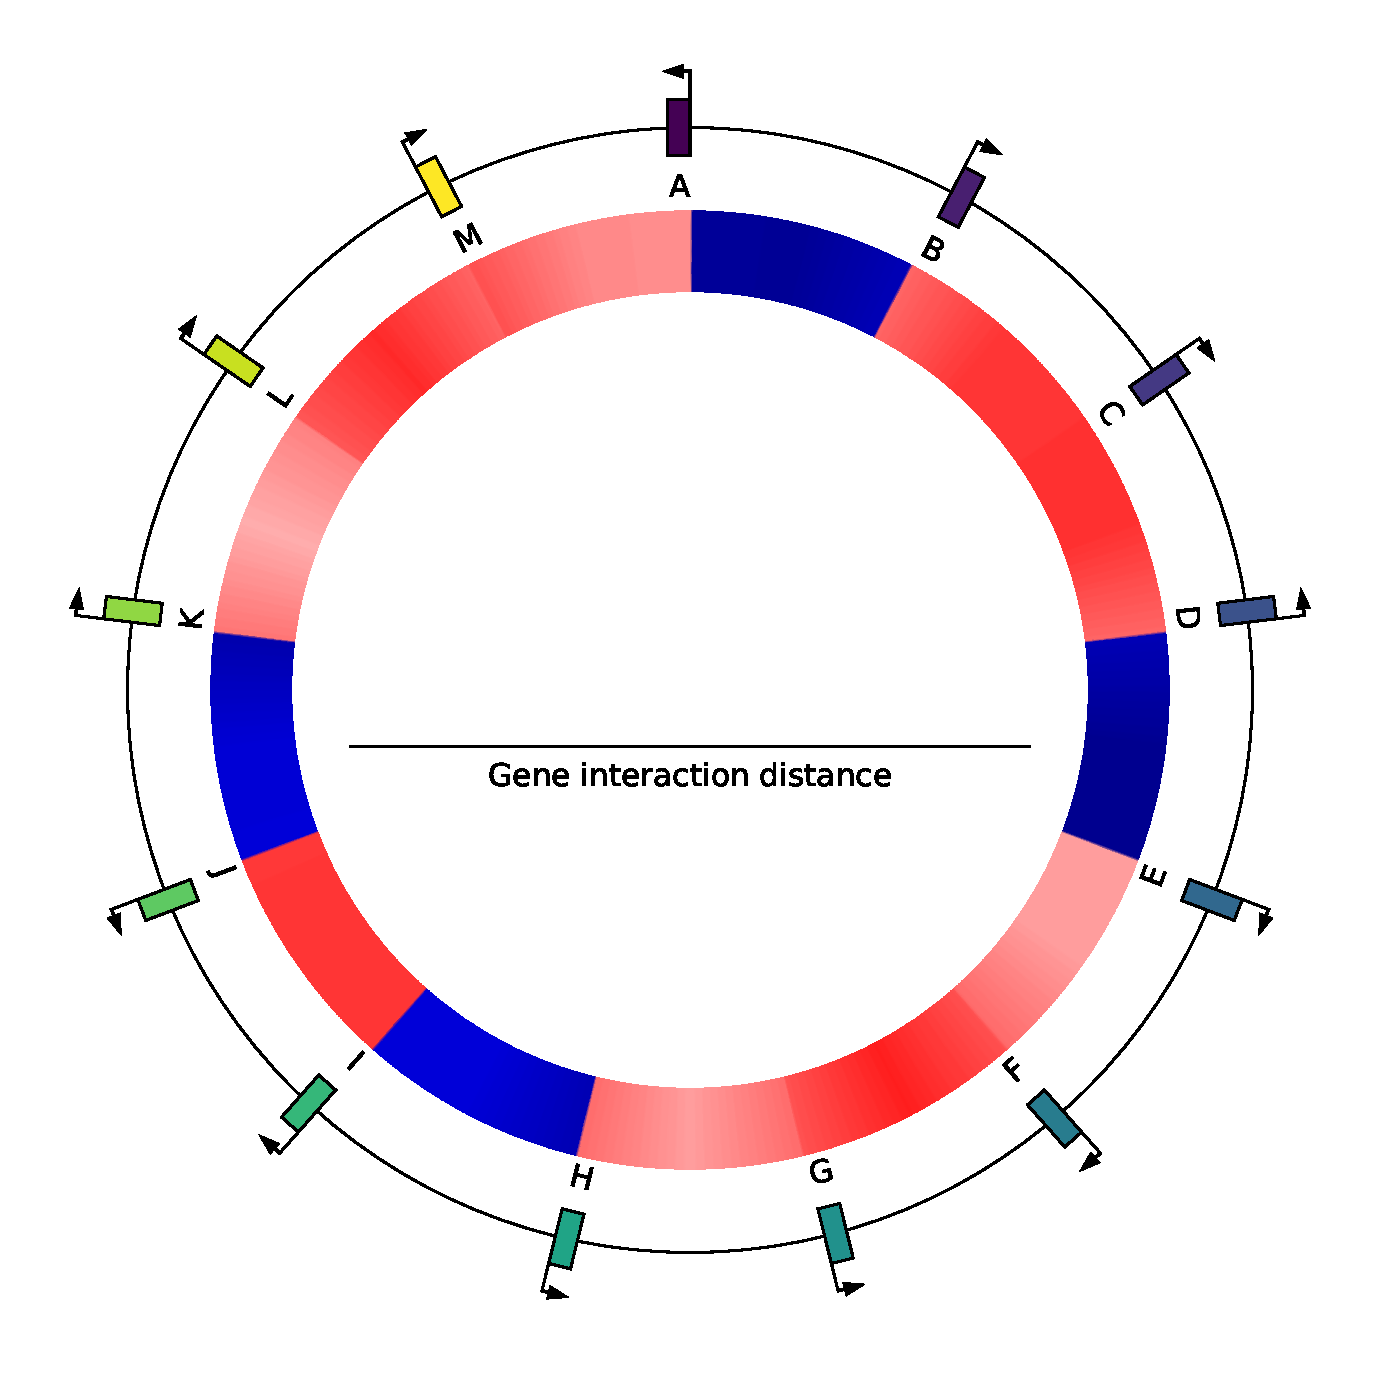
\includegraphics[width=\textwidth]{alife/img/13genes_genome_1.pdf}
\label{subfig:alife:genome_1}
\end{subfigure}
\hspace{-3mm}
\begin{subfigure}[t]{0.24\textwidth}
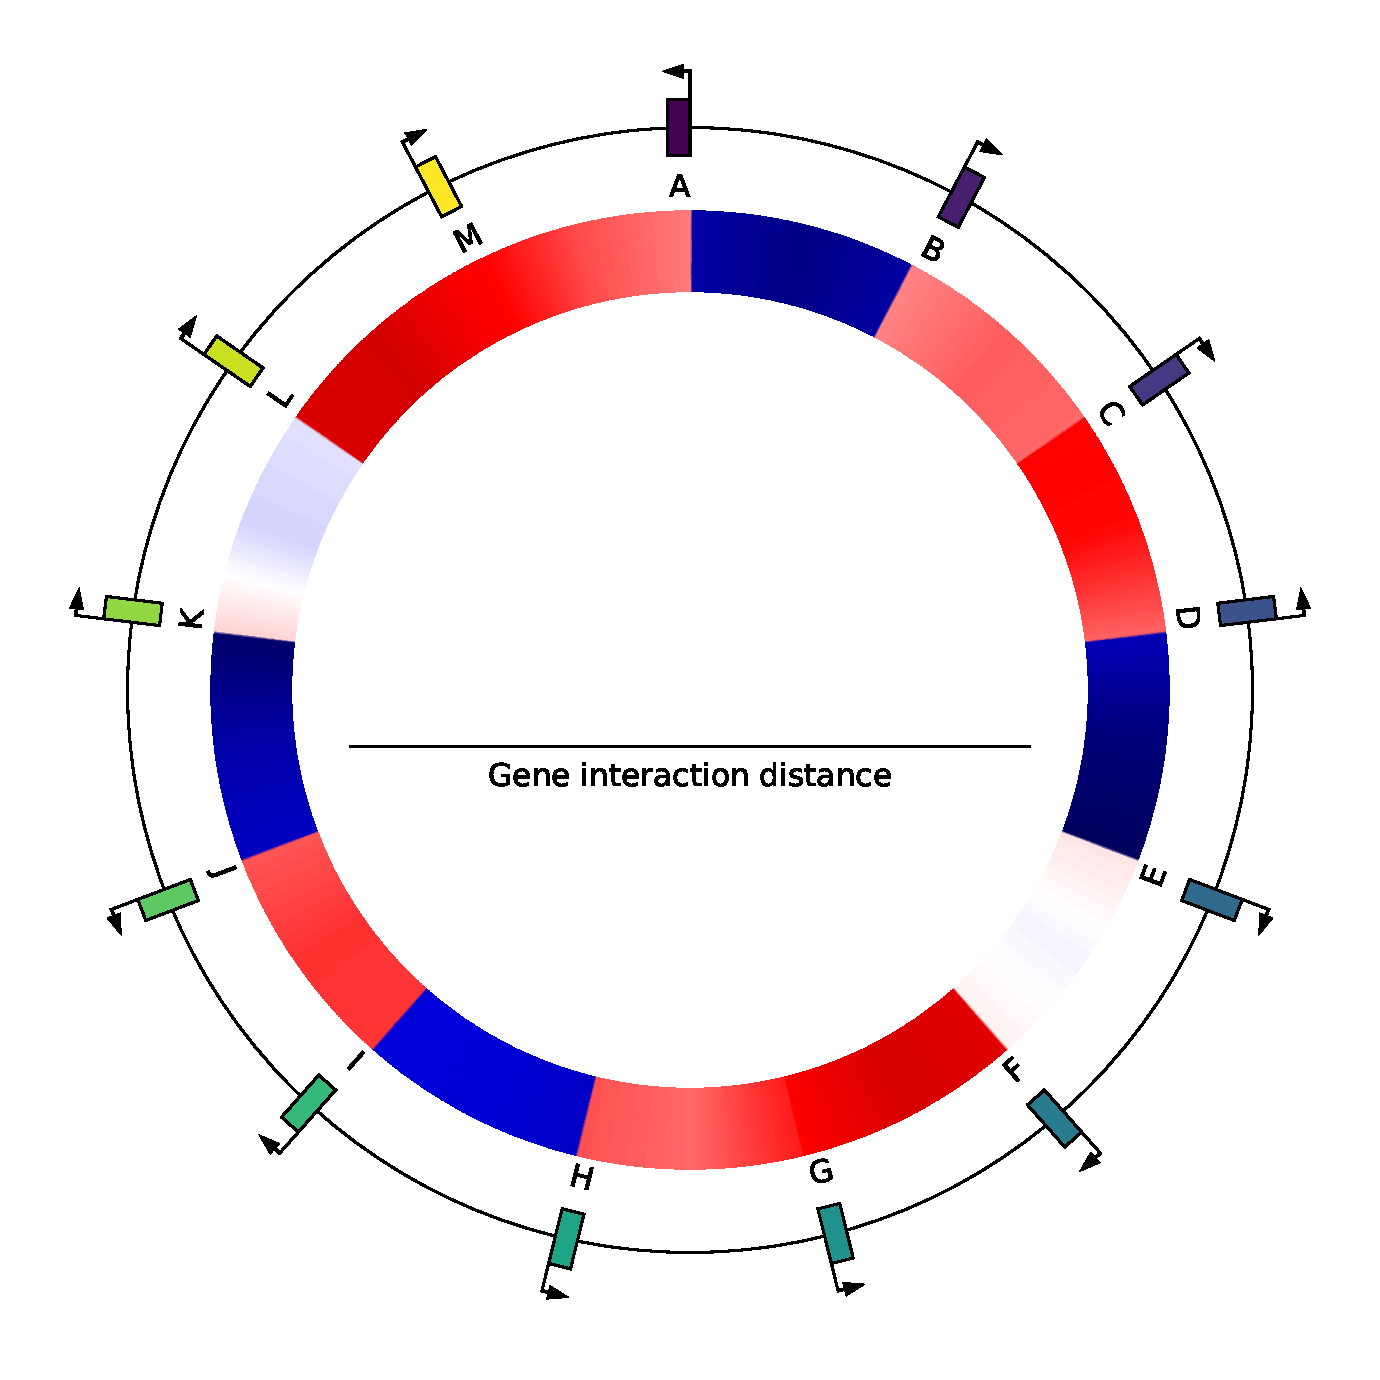
\includegraphics[width=\textwidth]{alife/img/13genes_genome_0.pdf}
\label{subfig:alife:genome_0}
\end{subfigure}
\vspace{-3mm}

\begin{subfigure}[t]{0.48\textwidth}
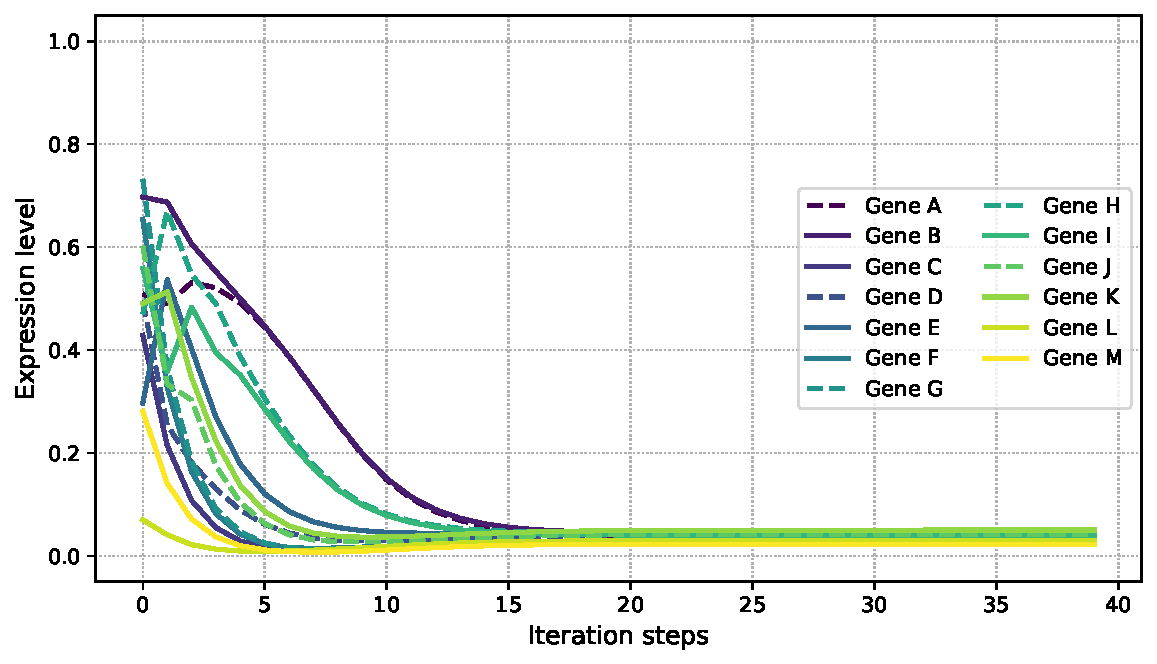
\includegraphics[width=\textwidth]{alife/img/13genes_sigma_3.pdf}
\label{subfig:alife:sigma_3}
\end{subfigure}
\begin{subfigure}[t]{0.48\textwidth}
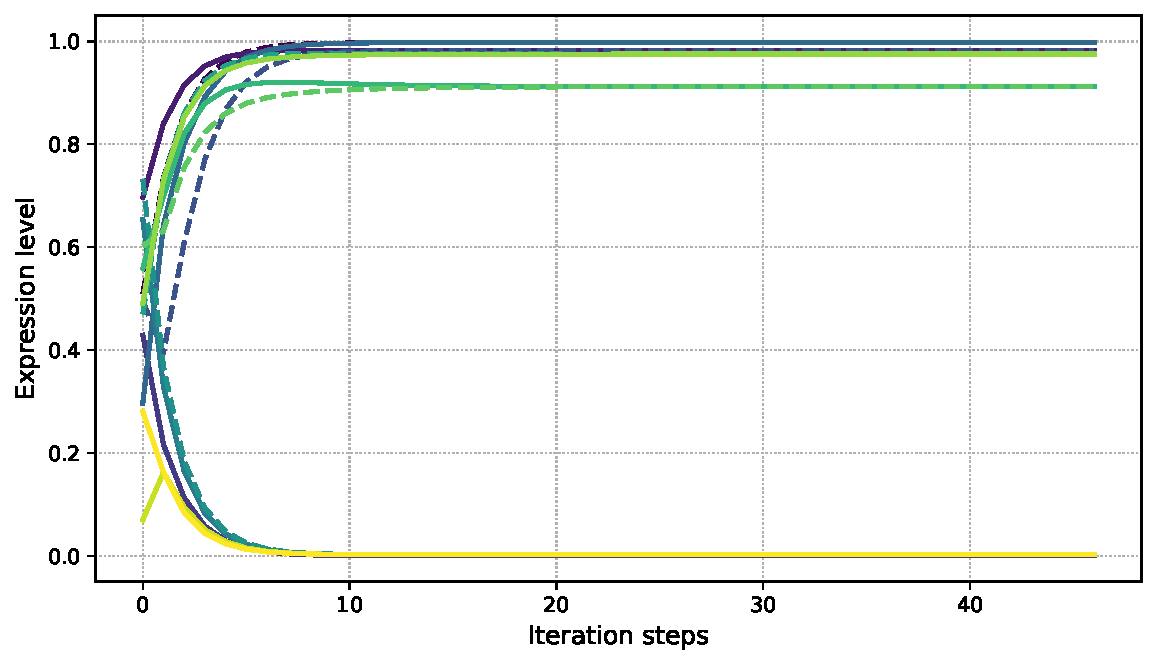
\includegraphics[width=\textwidth]{alife/img/13genes_sigma_2.pdf}
\label{subfig:alife:sigma_2}
\end{subfigure}
\vspace{-5mm}

\begin{subfigure}[t]{0.48\textwidth}
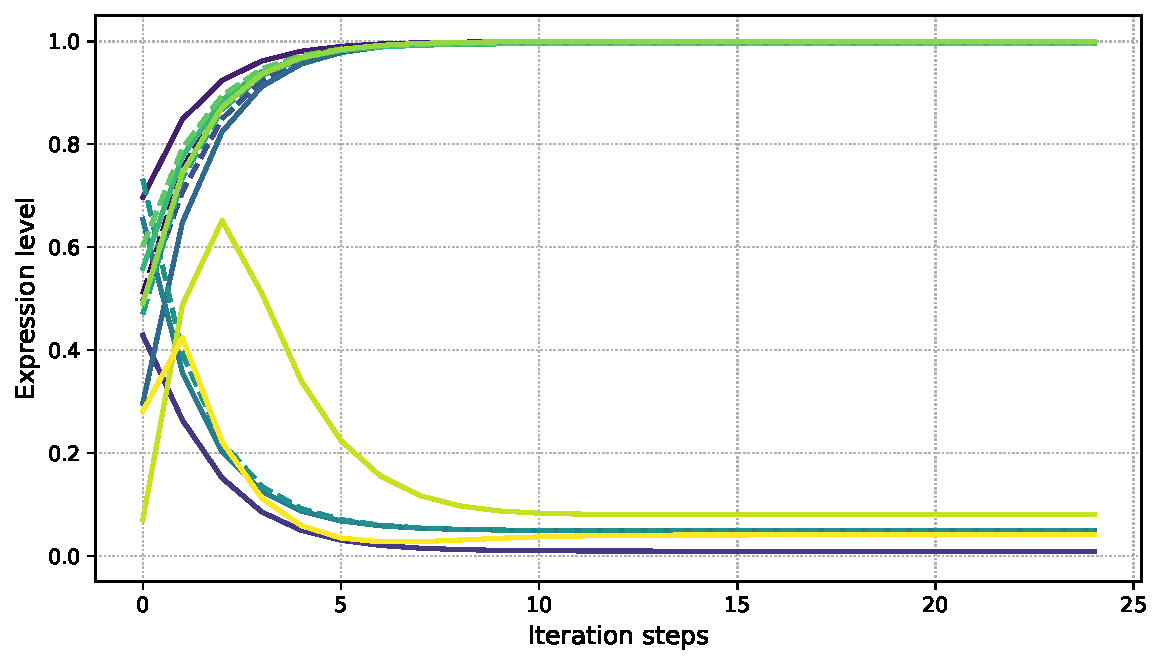
\includegraphics[width=\textwidth]{alife/img/13genes_sigma_1.pdf}
\label{subfig:alife:sigma_1}
\end{subfigure}
\begin{subfigure}[t]{0.48\textwidth}
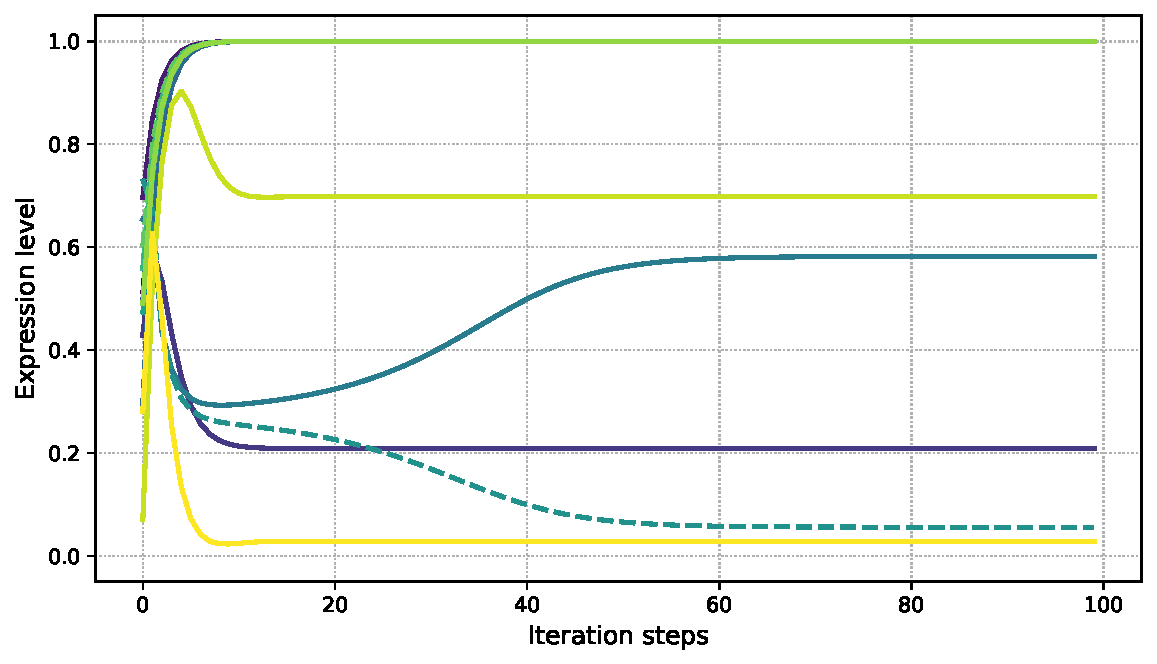
\includegraphics[width=\textwidth]{alife/img/13genes_sigma_0.pdf}
\label{subfig:alife:sigma_0}
\end{subfigure}
\caption[Influence of environmental supercoiling on the phenotype of the example individual in Figure~\ref{fig:alife:13genes}]{Influence of the environment supercoiling $\sigma_{env}$ on the stable state local supercoiling level (top row) and gene transcription levels (bottom rows) of the example individual.
From left to right and top to bottom: at $\sigma_{env} = 0.1$, no genes are activated ($e > 0.5$); at $\sigma_{env} = 0.0$ and at $\sigma_{env} = -0.1$, 8 genes are activated; at $\sigma_{env} = -0.2$, 10 genes are activated.
Lower values of $\sigma_{env}$ result in the activation of more genes, reflecting the \emph{in vivo} effect of higher negative supercoiling.}
\label{fig:alife:sigma_env}
\end{figure}

Figure~\ref{fig:alife:sigma_env} captures the influence of the environmental change in supercoiling $\sigma_{env}$ on the local supercoiling level due to the transcription-supercoiling coupling (top row) and on the repartition of genes between the activated and inhibited states (bottom rows), again using the example individual already shown in Figure~\ref{fig:alife:13genes}.
From left to right and top to bottom: at a high value of $\sigma_{env} = 0.1$, meaning that DNA is severely overwound compared to normal, no gene is activated (with an expression level $e > 0.5$) at all.
As the external influence of the environment on supercoiling decreases to $\sigma_{env} = 0$, corresponding to normal relaxation of DNA, and then to $\sigma_{env} = -0.1$, 8 out of the 13 genes of the individual reach an activated state.
Finally, for $\sigma_{env} = -0.2$, there is a strong environmental pressure towards high gene transcription levels, and most genes are indeed activated; however, even at this level of $\sigma_{env}$, some genes remain shut down, because of the high amount of positive supercoiling (in red) generated by the transcription of their neighbors.


\subsection{Influence of Relative Gene Positions on Gene Activation Levels}
\label{sec:alife:gene_pos}

\begin{figure}[H]
\centering
\begin{subfigure}[t]{0.42\textwidth}
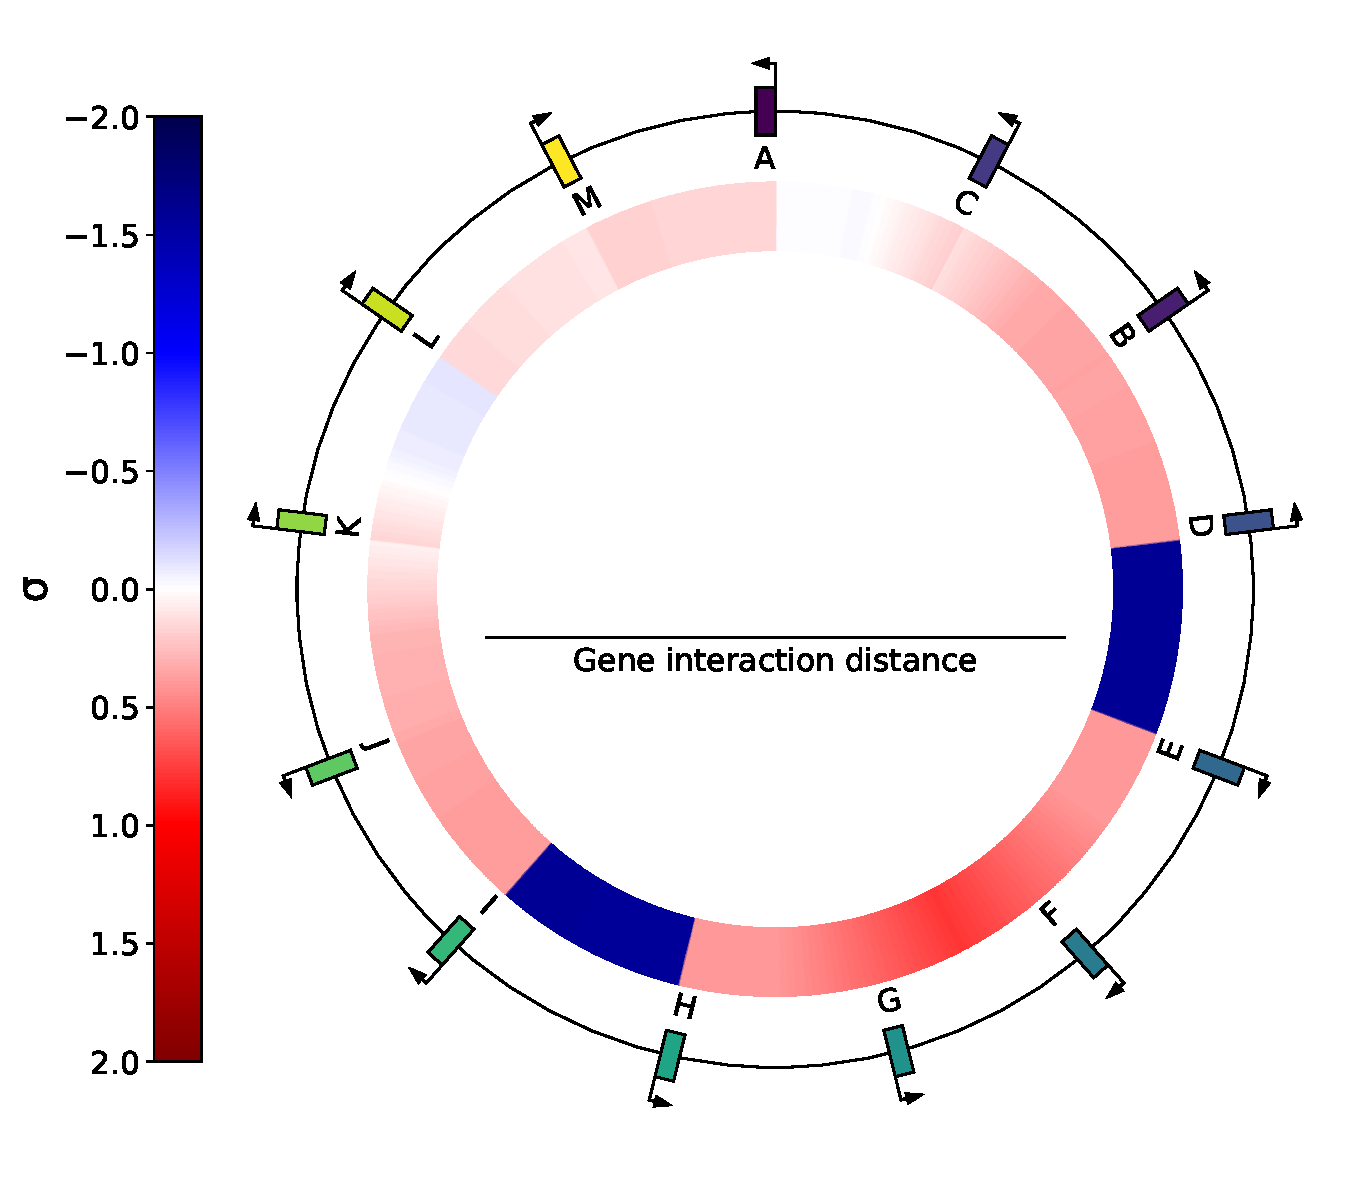
\includegraphics[width=\textwidth]{alife/img/inversion_genome.pdf}
\label{subfig:alife:inversion_genome}
\end{subfigure}
\begin{subfigure}[t]{0.56\textwidth}
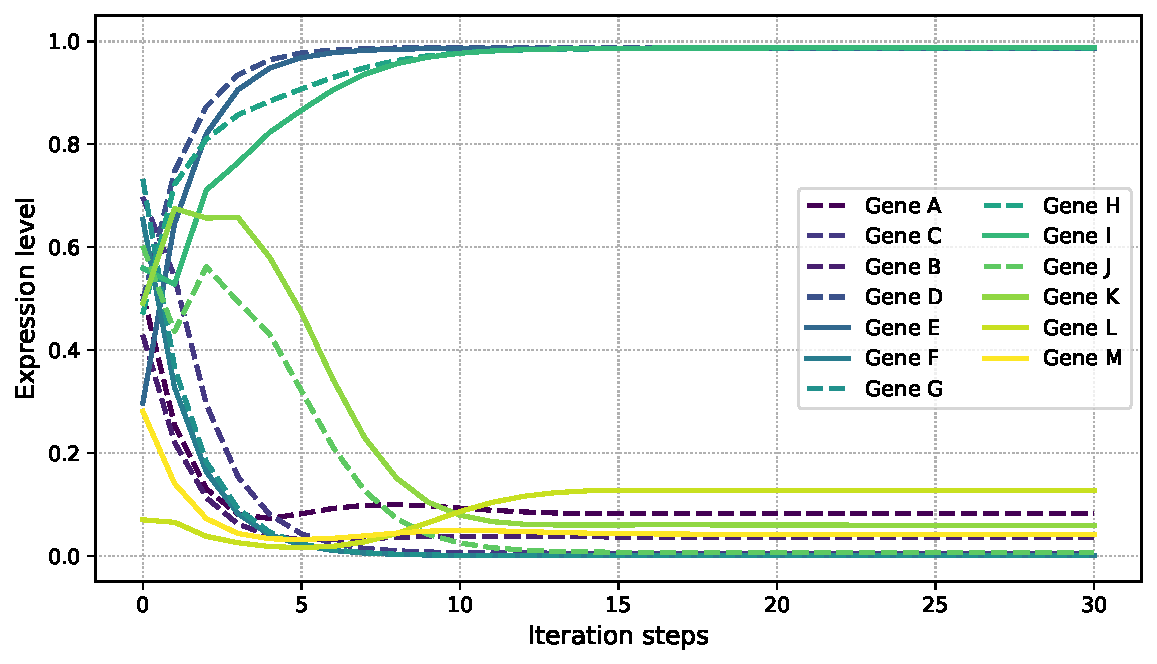
\includegraphics[width=\textwidth]{alife/img/inversion_expr_level.pdf}
\label{subfig:alife:inversion_expr}
\end{subfigure}
\caption[Effect of a genomic inversion on the example individual in Figure~\ref{fig:alife:13genes}]{Genome, local supercoiling and gene expression levels of a new individual obtained from the individual in Figure~\ref{fig:alife:13genes} by switching the positions and orientations of genes B and C.}
\label{fig:alife:inversion}
\end{figure}

Figure~\ref{fig:alife:inversion} again shows the local supercoiling and gene expression levels of the individual in Figure~\ref{fig:alife:13genes}, after reversing the positions and orientations of genes B and C.
This is an example of a genomic inversion, which will be presented in further detail in section~\ref{sec:inversion}.
The starting point of this inversion falls between genes A and B and its end point between genes C and D; this results in the reversal of segment [BC] relative to the rest of the genome.
Here, we can see that the diverging orientation that was present between genes A and B has vanished, replaced by a set of genes in colinear orientation, from A to D.
This genomic reorganization results in the loss of the activation of genes A and B, as gene B is now more strongly inhibited by gene D due to its closer genomic location, and as genes A and B are not in a positive feedback loop -- due to diverging orientations -- any longer; only the pairs of genes D and E, and H and I, remain activated.

Based on these observations, we can confirm that in our model, the transcription"=supercoiling coupling generates complex networks of genome-wide interactions between genes, and that these networks directly depend on the architecture of the genome.


\section{An Evolutionary Genome-Wide Model of the Transcription-Supercoiling Coupling}
\sectionmark{An Evolutionary Genome-Wide Model of the TSC}
\label{sec:alife:evol_model}

After evidencing that transcriptional activity depends on the organization of the genome, we now question to which extent evolution can simultaneously leverage the organization of the genome and the transcription-supercoiling coupling in order to adapt gene regulatory activity to different environments.
Indeed, as has been observed in \emph{Dickeya dadantii}~\citep{muskhelishvili2019}, different phenotypes can evolve as a response to different supercoiling levels induced by the environment, and the transcription-supercoiling coupling could play a role in enabling the existence of this reaction norm.

In this section, we expand our model into an evolutionary simulation.
At each generation of the simulation, all individuals are evaluated and their fitness values are computed, based on their gene transcription levels.
Then, the individuals of the new generation are chosen by picking their ancestor from the current generation, with a probability proportional to the ancestor's fitness.
The model is panmictic, meaning that any individual in the population can be chosen as the ancestor of any new individual.
Finally, during replication, the genome of each new individual stochastically undergoes a number of mutations, before the new individual is evaluated again; importantly, these mutations do not impact genes themselves, but only the spatial organization of the genome: gene orientations, syntenies, and intergenic distances.

\subsection{Evolutionary Model: Evolution in Two Separate Environments}

We model the evolution of populations of individuals that experience two different environments, named A and B.
Each environment is defined by its value of $\sigma_{env}$, respectively $\sigma_A$ and $\sigma_B$, which represent the change in the supercoiling level due to the environment~\citep{dorman2016}.
In order to have environments with distinct effects, we choose a value of $\sigma_A = 0.1$, for which isolated genes are effectively inhibited (as in the top-left panel of Figure~\ref{fig:alife:sigma_env}), and a value of $\sigma_B = -0.1$, for which some but not all genes are activated (bottom-left panel).

We separate genes into three classes, based on the environments in which they must be activated: either in both environment A and environment B (\emph{AB} genes), only in environment A (\emph{A} genes), or only in environment B (\emph{B} genes).
These classes allow us to define optimal phenotypes for both environments: in environment A, both \emph{A} and \emph{AB} genes should be activated, whereas \emph{B} genes should be inhibited.
Conversely, in environment B, only \emph{B} and \emph{AB} genes should be activated, but not \emph{A} genes.


\subsection{Fitness}

In order to compute the fitness of an individual, we define an optimal phenotype $\tilde{e}^A$ (resp. $\tilde{e}^B$), corresponding to the vector of the expected expression level $\tilde{e}^A_i$ for each gene $i$ in environment A (resp. environment B).
We choose an expected expression level of $\tilde{e} = 1$ for genes that should be activated, which corresponds to the maximum possible expression level of a gene in our model.
Similarly, we choose $\tilde{e} = 0$ for genes that should be inhibited, which is the minimum expression level that is attainable.
Then, in each environment, we compute the gap $g_A$ (resp. $g_B$), or average square distance of the individual's gene transcription levels $e^A$ (the vector constituted by the transcription level $e^A_i$ of each gene $i$) to the optimal levels $\tilde{e}^A$ (resp. $e^B$ and $\tilde{e}^B$).
The gap $g_A$ is computed as follows:

\begin{equation}
g_A(e^A) = \frac{1}{n} \sum_{i=1}^{n} (e^A_i - \tilde{e}^A_i)^2
\label{eq:alife_gap}
\end{equation}

The gap $g_B$ is computed in the same way.
Finally, we compute the fitness of the individual by summing the gap in each environment, and applying an exponential scaling: $f = e^{-k (g_A + g_B)}$, where $k$ is a scaling factor representing the selection pressure.
A higher value of $k$ means that well-adapted individuals, those which have a smaller gap, will have an even higher fitness value compared to other individuals; we typically use $k=50$, meaning that a small decrease in the gap compared to other individuals yields a large reproductive advantage.


\subsection{Mutational Operator: Genomic Inversions}
\label{sec:inversion}

We introduce only one kind of mutation in our model, which is genomic inversions: we choose two breakpoints randomly on the genome, and reverse the genomic content between these points.
Genes are then reinserted in the genome in the opposite orientation and order, taking care to update all intergenic distances appropriately.
Note that in our model, genes have a length of zero and the breakpoints can therefore not fall inside a gene.
Moreover, an inversion has no effect if both breakpoints fall between two neighboring genes (as only an intergenic region would be affected), but can impact any number of genes otherwise.
Genomic inversions hence affect gene syntenies and orientations, and therefore affect gene expression levels as presented in subsection~\ref{sec:alife:gene_pos}.
When mutating a genome during reproduction, we draw the number of inversions $k$ to perform from a Poisson law with parameter $\lambda = 2$, giving an average of 2 inversions between an individual and its ancestor; the probability of not undergoing any mutations is $P(k=0) = e^{-\lambda} \approx 0.136$.

\begin{figure}[H]
\centering
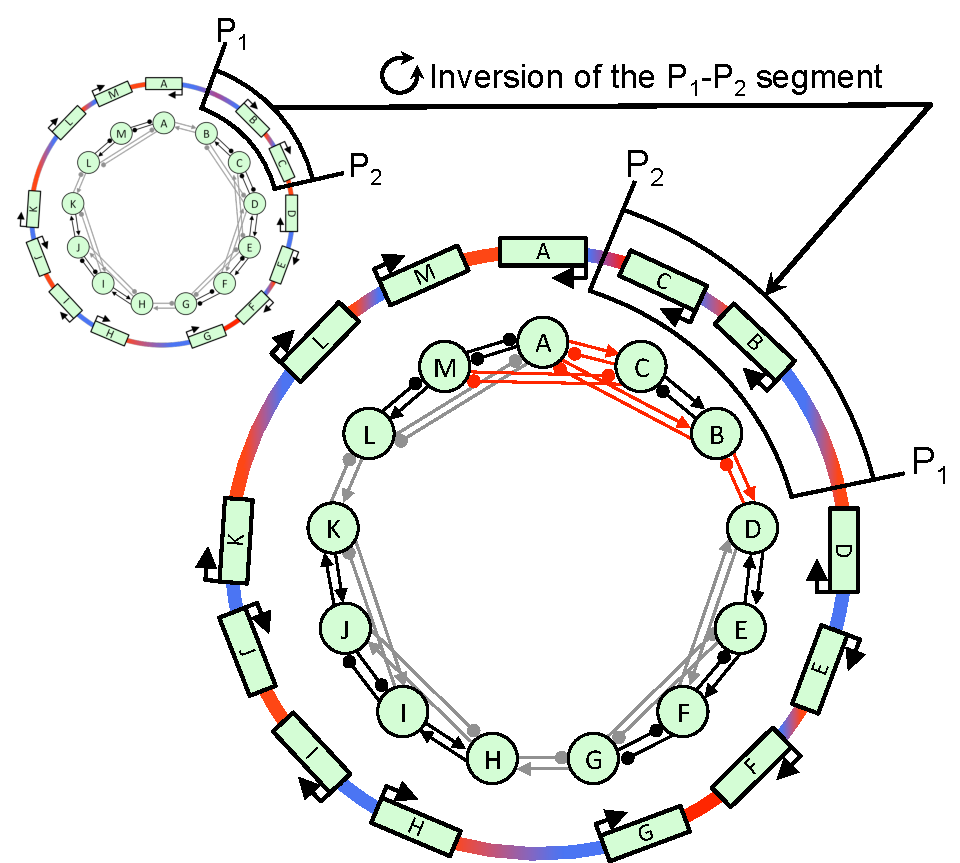
\includegraphics[width=0.8\textwidth]{alife/img/genome_inversion.pdf}
\caption[Effect of an inversion on the hand-drawn genome in Figure \ref{fig:alife:network}]{Result of the inversion of a genomic segment containing genes B and C from the individual presented in Figure~\ref{fig:alife:network}.
The gene interactions which have changed due to the inversion are drawn in red.
This illustration genome corresponds to the actual individual in our model presented in Figure~\ref{fig:alife:inversion}.}
\label{fig:alife:genome_inv}
\end{figure}

Figure \ref{fig:alife:genome_inv} presents a genome obtained by performing an inversion on the genome shown in Figure~\ref{fig:alife:network}.
As a result of this inversion, genes B and C have been switched from the forward to the backward orientation, and the intergenic distances between A and C on the one hand, and B and D on the other hand, have been modified; however, the relative orientation of B and C, and hence their interaction subnetwork, remain unchanged.
This results in changes to the gene interaction network: instead of mutual activation between genes A and B and mutual inhibition between genes C and D, all four genes now lie in colinear orientations, in which each of these genes activates its upstream neighbor but represses its downstream neighbor.

\subsection{Experimental Setup and Parameter Values}

We initialized the simulation with a clonal population of $N=100$ copies of an initial individual with the following genome: 60 genes in random orientations, uniformly distributed along a 60,000 bp genome, and equally divided between the \emph{AB}, \emph{A} and \emph{B} classes.
We chose a maximum interaction distance of $d_{max} = 2500$, meaning that each gene initially interacts with its 2 closest neighbors in each direction through the transcription-supercoiling coupling.
Note that as inversions may change intergenic distances, genes can move closer or further apart during evolution.
We set the basal supercoiling level $\sigma_{basal}$ to the average supercoiling level in \emph{E. coli} of -0.06~\citep{crozat2005}, and $\sigma_0$ to $-0.06$ as well, so that in the absence of other sources of supercoiling (either environmental or through the coupling), the default activity level of a gene is 0.5.
Finally, we set $c = 0.3$, in order to have comparable values for the variations in supercoiling due to the environment and due to the transcription-supercoiling coupling, and $\epsilon=0.03$, so that the variations in supercoiling have a qualitatively mild effect on gene expression.

In order to run the simulations, we evolved 15 different populations for 250,000 generations; the simulation lasted for approximately 48h on a computer with Intel Xeon E5-2640 v3 @ 2.60GHz CPUs, using around 100 MB of RAM per replicate.
All the data from the experiment is available online on the \href{https://doi.org/10.5281/zenodo.6556310}{Zenodo} platform.

\subsection{Adaptation of Gene Expression Levels to Different Environments}

Figure~\ref{fig:alife:mean_activ} summarizes the differences in the proportion of activated genes for each of the three sets of genes, between environments A and B, averaged over the 15 repetitions.
In the figure, we consider a gene to be activated if its activity at the end of the lifecycle is over $0.5$, and we look at the average proportion of activated genes in the best individual of every replica.
Let us recall that the evolutionary target for \emph{AB} genes is an expression level of 1 in both environments, for \emph{A} genes an expression level of 1 in environment \emph{A} and 0 in \emph{B}, and vice-versa for \emph{B} genes.
After 250,000 generations of evolution, individuals have acquired genomes that allow all \emph{AB} genes to be activated in both environments, and that allow all \emph{B} genes to be activated in environment B and inhibited in environment A.
On average, over 60\% of \emph{A} genes are activated in environment A, which imposes a positive change in supercoiling ($\sigma_A = 0.1$) and makes gene activation harder.
Conversely, less than 5\% of \emph{A} genes are activated in environment B, in which gene activation is easier ($\sigma_B = -0.1$).
The final expression levels of \emph{A} genes therefore show that specific sets of genes can be activated by the transcription-supercoiling coupling despite environmental hurdles.

\begin{figure}[H]
\centering
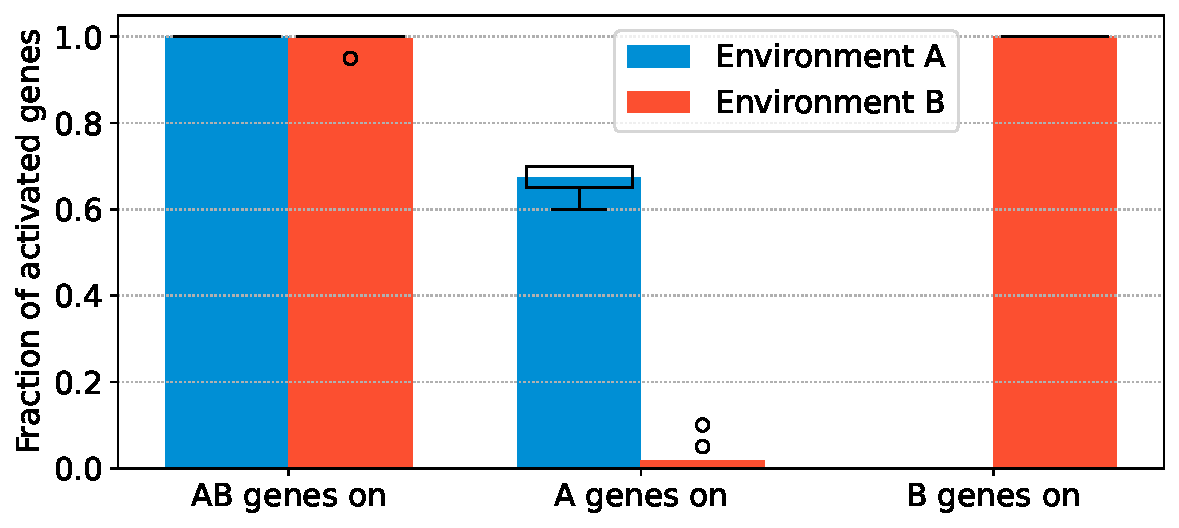
\includegraphics[width=0.8\textwidth]{alife/img/mean_activation.pdf}
\caption[Fraction of activated genes of each type at the end of evolution in the proof-of-concept model]{Fraction of activated genes of each type in each environment at the end of the lifecycle, averaged over the best individuals in the last generation of each replica.
The boxplots represent the median and quartiles, and the dots flier data points.
For \emph{A} genes and \emph{B} genes, activation levels differ depending on the environment: $p$-value $2.40\times10^{-17}$ for \emph{A} genes, and $p$-value $<1\times10^{-25}$ for \emph{B} genes (Student's $t$-test for dependent samples).}
\label{fig:alife:mean_activ}
\end{figure}

Furthermore, in each of the 15 replicates, the fitness of the best individual in the population increases continuously over the course of evolution, as shown in Figure~\ref{fig:alife:fitnesses}.
As their respective fitness keeps increasing until the end of the simulation, this suggests that fitter phenotypes remain reachable through further evolution by genomic rearrangements.
The rhythm of evolution is however progressively slower and slower (note the logarithmic time scale in the figure), as the pool of available favorable mutations decreases.

\begin{figure}[H]
\centering
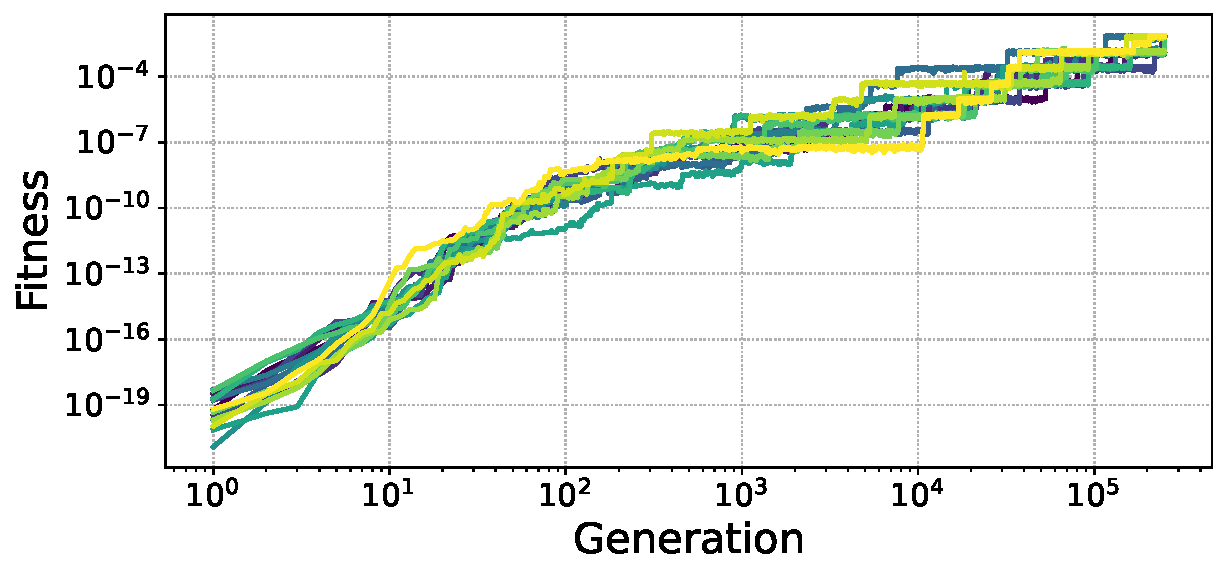
\includegraphics[width=0.8\textwidth]{alife/img/all_fitness.pdf}
\caption[Fitness of every replicate during evolution in the proof-of-concept model]{Evolution of the fitness of the best individual of each replicate at every generation.}
\label{fig:alife:fitnesses}
\end{figure}

Finally, details of the evolution of one of the 15 replicate populations are shown in Figure~\ref{fig:alife:evolution}.
We can first see that the number of activated \emph{AB} genes of the best individual at each generation quickly rises to 20 (out of 20 genes of that type) in both environment A and environment B; this shows that evolving a phenotype that is resistant to environmental perturbations, having genes that are always activated, is easy in the model.
For \emph{A} genes and \emph{B} genes, we observe an asymmetric tendency during the course of evolution towards activation in the target environment, and inhibition in the opposite environment.
However, the difference in the number of activated \emph{B} genes between environment A and environment B is much higher than for \emph{A} genes.
As already mentioned above, this asymmetry comes from the different requirements expected of \emph{A} genes and \emph{B} genes: gene activation is easier in environment B than in environment A, as it is easier for a gene to become activated in an environment with a lower overall supercoiling level.
\emph{A} genes therefore have to be activated in a harder environment, and inhibited in a simpler environment, whereas \emph{B} genes have to do the opposite.

\begin{figure}[H]
\centering
\begin{subfigure}[t]{0.8\textwidth}
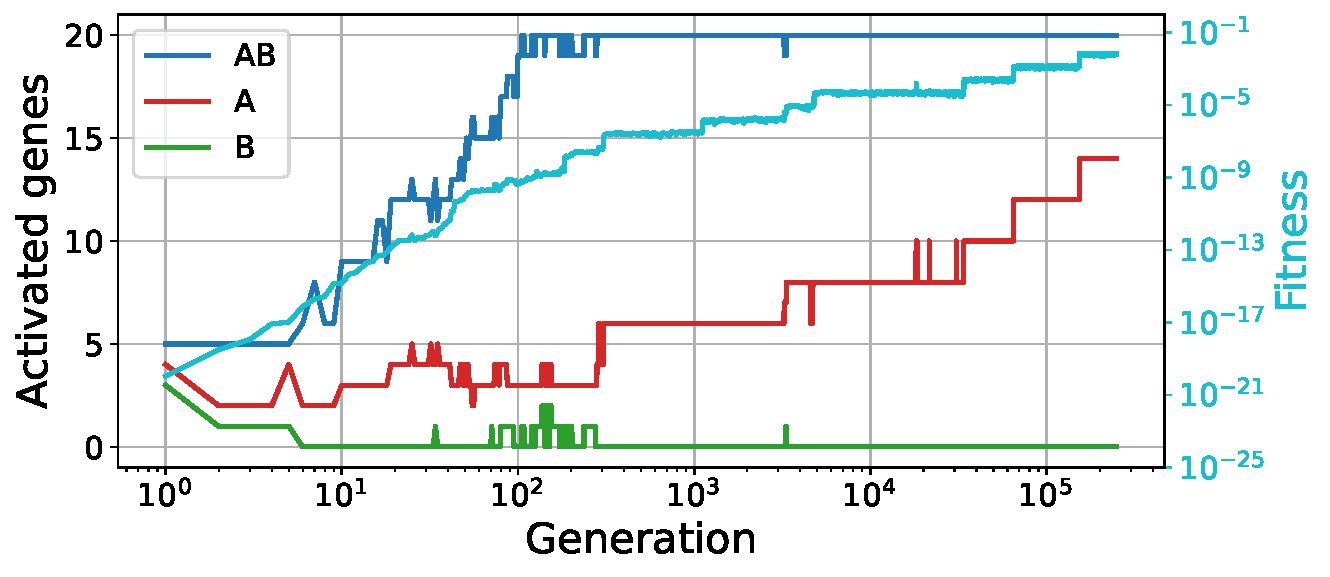
\includegraphics[width=\textwidth]{alife/img/rep_13_env_A.pdf}
\label{subfig:alife:env_A}
\end{subfigure}

\begin{subfigure}[t]{0.8\textwidth}
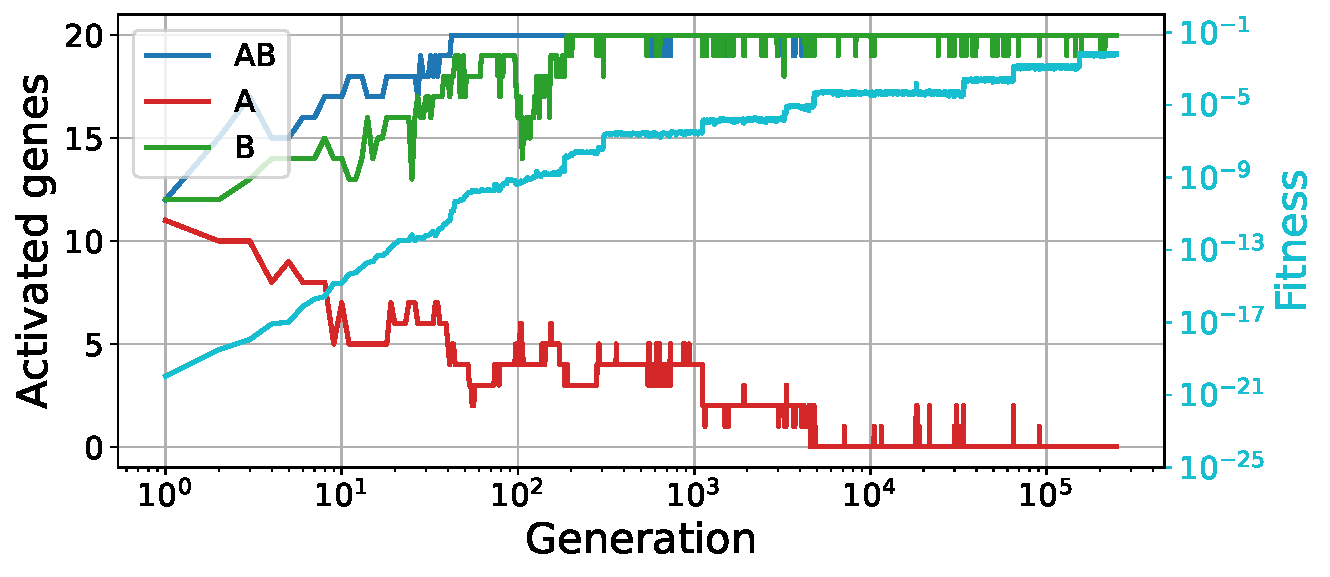
\includegraphics[width=\textwidth]{alife/img/rep_13_env_B.pdf}
\label{subfig:alife:env_B}
\end{subfigure}

\caption[Number of activated genes during evolution in one of the replicates in the proof-of-concept model]{Number of activated genes of each type and fitness of the best individual at every generation of replicate 13, with a population size of $N=100$, for 250,000 generations.
The number of active \emph{AB} genes increases until it reaches 20, in both environment A (top) and environment B (bottom).
The number of active \emph{A} (resp. \emph{B}) genes increases in environment A (resp. B) and decreases in environment B (resp. A) over time, thus converging towards their evolutionary target.}
\label{fig:alife:evolution}
\end{figure}

This is shown in more detail in Figure~\ref{fig:alife:best_indiv}, which shows the supercoiling level and gene activation levels of the best individual of the last generation of replicate 13, in both environments.
The phenotypes displayed in each environment present clearly distinct gene expression patterns.
In environment A (top), nearly all genes converge directly towards their final state, whereas in environment B (bottom), most \emph{A} genes (in red) and some \emph{B} genes (in green) show a complex trajectory of activation levels before reaching their stable state.
Moreover, genomic domains with markedly different supercoiling levels emerge through the transcription-supercoiling coupling, with both very overwound and very underwound zones.
These domains also show qualitatively different responses to different environments: in some domains, the supercoiling level is very similar (around gene 0, gene 15 or gene 55 for example), while in others supercoiling is completely different in each environment (between genes 20 and 35).
This shows the plasticity of the response to environmental change at the local supercoiling level.

\begin{figure}[H]
\centering
\begin{subfigure}[t]{0.42\textwidth}
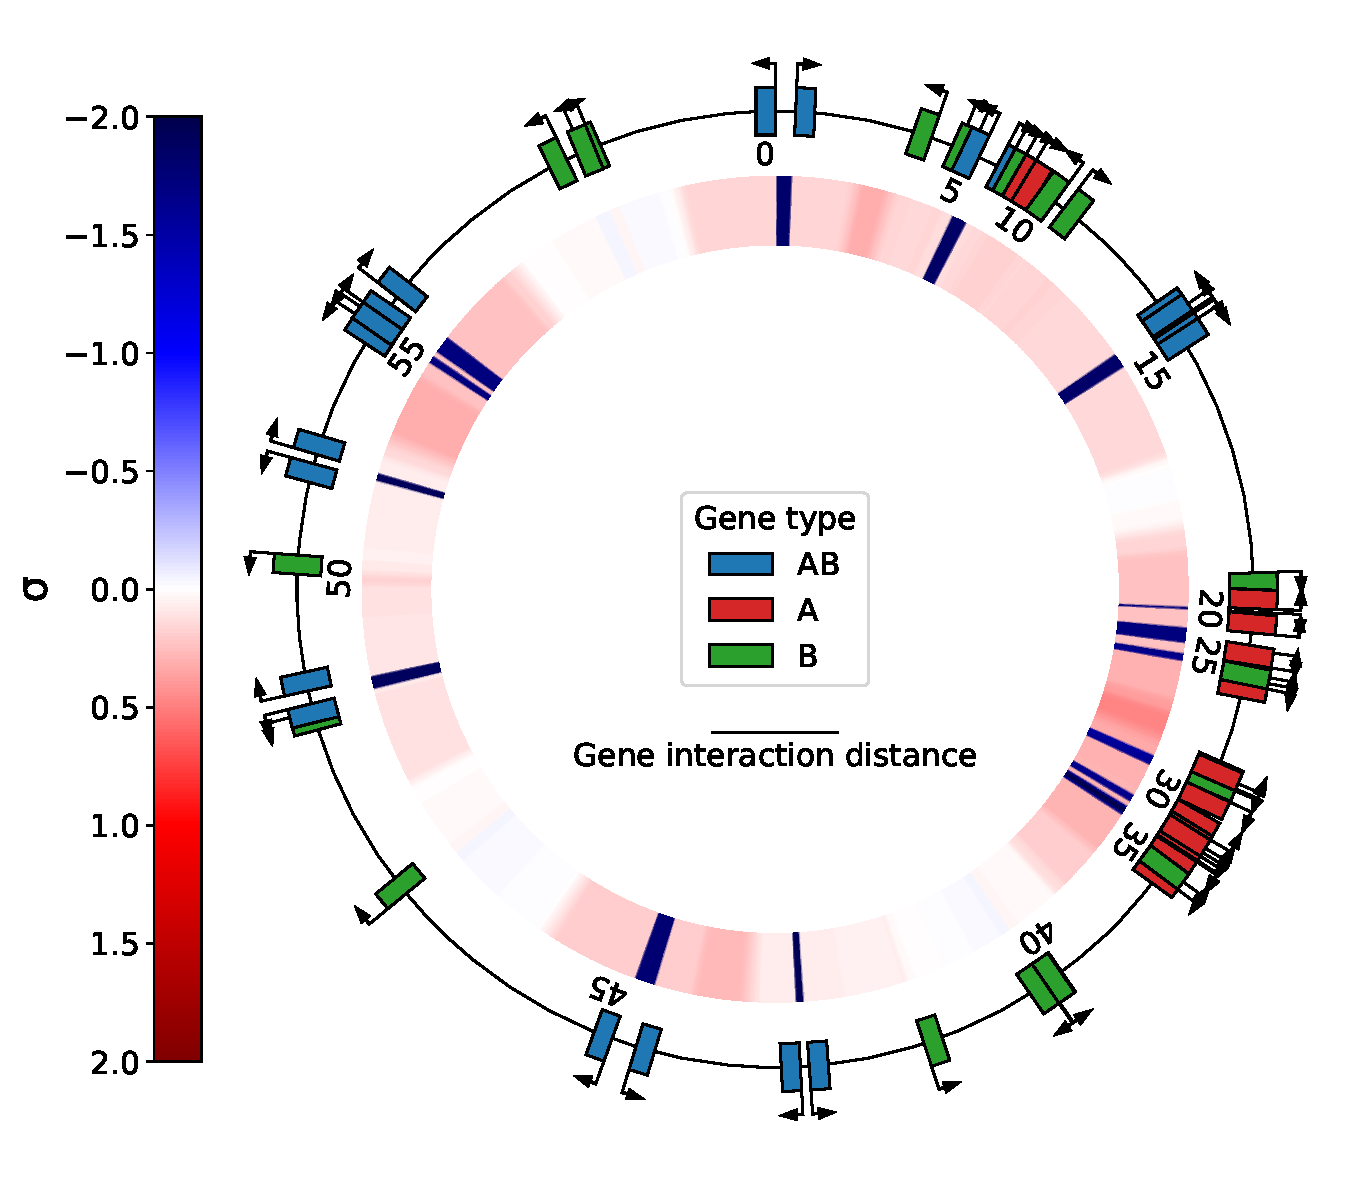
\includegraphics[width=\textwidth]{alife/img/genome_and_tsc_rep13_env_A.pdf}
\label{subfig:alife:best_genome_A}
\end{subfigure}
\begin{subfigure}[t]{0.56\textwidth}
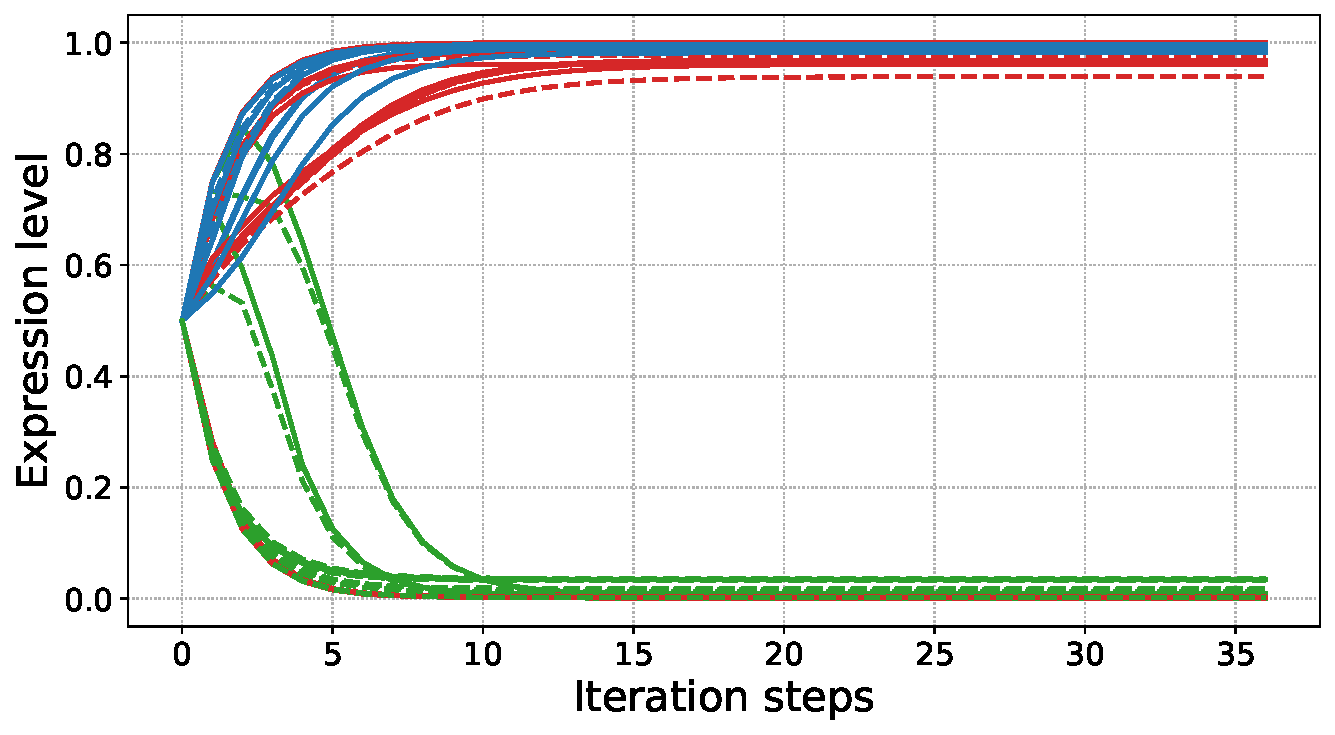
\includegraphics[width=\textwidth]{alife/img/best_rep13_env_A.pdf}
\label{subfig:alife:best_expr_A}
\end{subfigure}
\vspace{-5mm}

\begin{subfigure}[t]{0.42\textwidth}
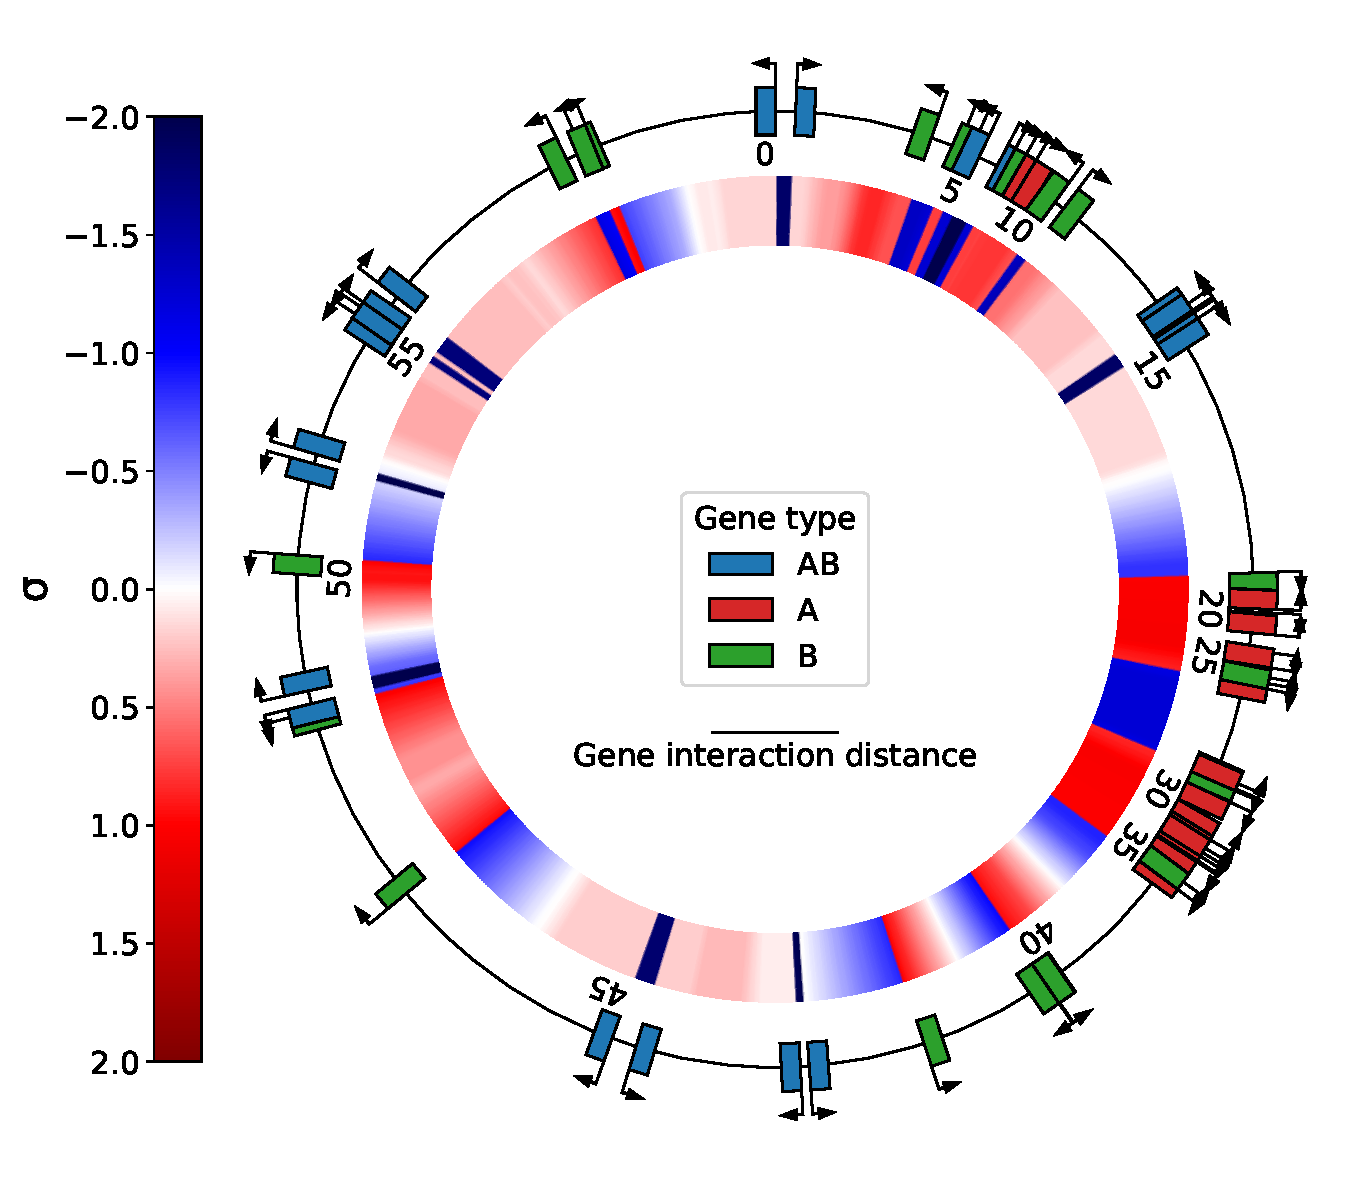
\includegraphics[width=\textwidth]{alife/img/genome_and_tsc_rep13_env_B.pdf}
\label{subfig:alife:best_genome_B}
\end{subfigure}
\begin{subfigure}[t]{0.56\textwidth}
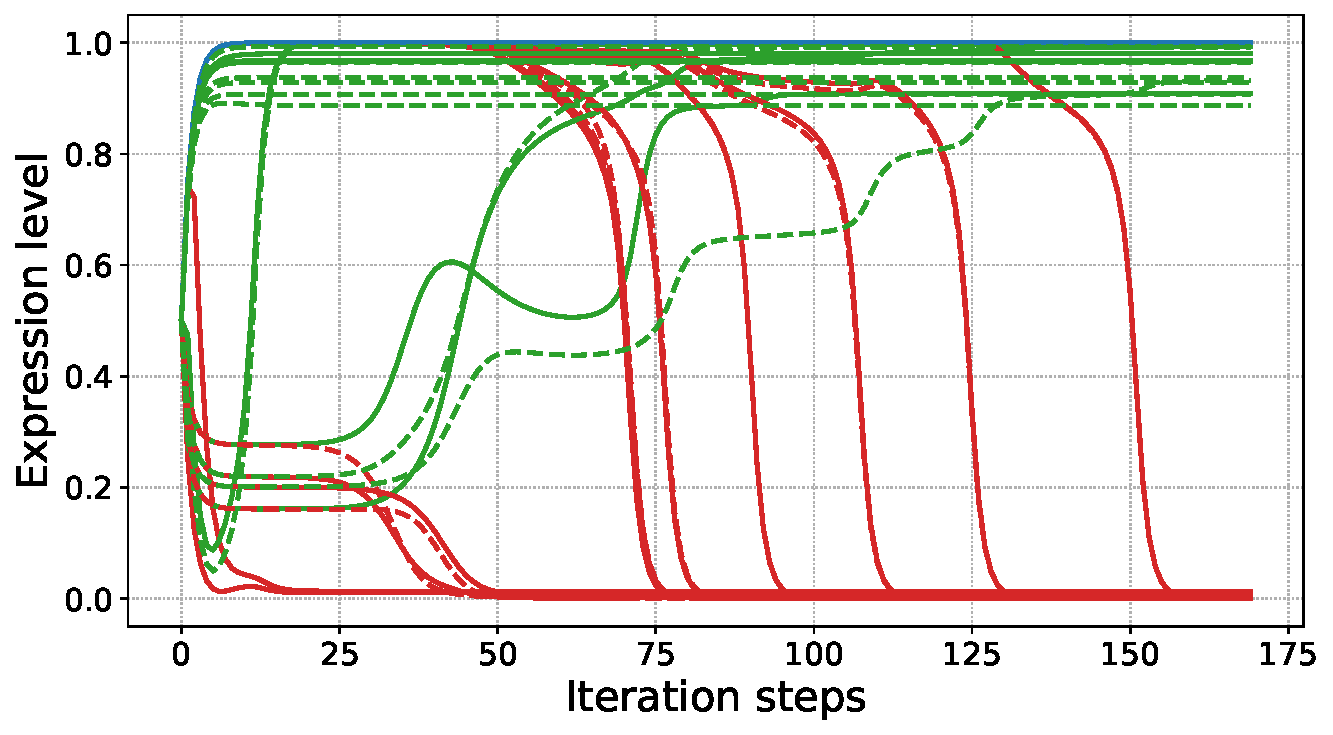
\includegraphics[width=\textwidth]{alife/img/best_rep13_env_B.pdf}
\label{subfig:alife:best_expr_B}
\end{subfigure}
\caption[Best individual at the end of evolution in one of the replicates in the proof-of-concept model, evaluated in both environments]{Local supercoiling along the genome and gene transcription levels of the best individual in replicate 13 after 250,000 generations.
Environment A is on top and environment B at the bottom.
\emph{AB} genes are colored blue, \emph{A} genes colored red, and \emph{B} genes colored green.}
\label{fig:alife:best_indiv}
\end{figure}

Our experimental results show that, in a model of gene transcription that is structured around the transcription"=supercoiling coupling, complex gene interaction networks can in fact evolve.
These gene interaction networks are sensitive to environmental variations, which are mediated in our model by a single parameter: $\sigma_{env}$, the amount of global supercoiling that is due to the environment.

\subsection{Robustness of Gene Network Evolution}
\label{sec:alife:param_explor}

In order to ensure that our results remain experimentally valid over a broad range of parameter values, we ran additional sets of simulations.
We changed respectively the sensitivity of gene promoters to supercoiling changes ($\epsilon$ in equation~\ref{eq:transcr}), the interaction coefficient used in computing the local supercoiling due to the transcription-supercoiling coupling ($c$ in equation~\ref{eq:dsde}), and the strength of the change in supercoiling imposed by the environment ($\sigma_A$ and $\sigma_B$).
We chose sets of logarithmically-spaced values for each parameter, and ran 5 replicates of the evolution experiment for 250,000 generations for each parameter value.
Note that, for extreme parameter values, gene expression levels did in some cases not converge to stable states by the maximum number of computation steps.
In this situation, we chose to retain the gene expression levels at the last step as the phenotype of the affected individuals.

\begin{figure}[H]
\centering
\begin{subfigure}[t]{0.49\textwidth}
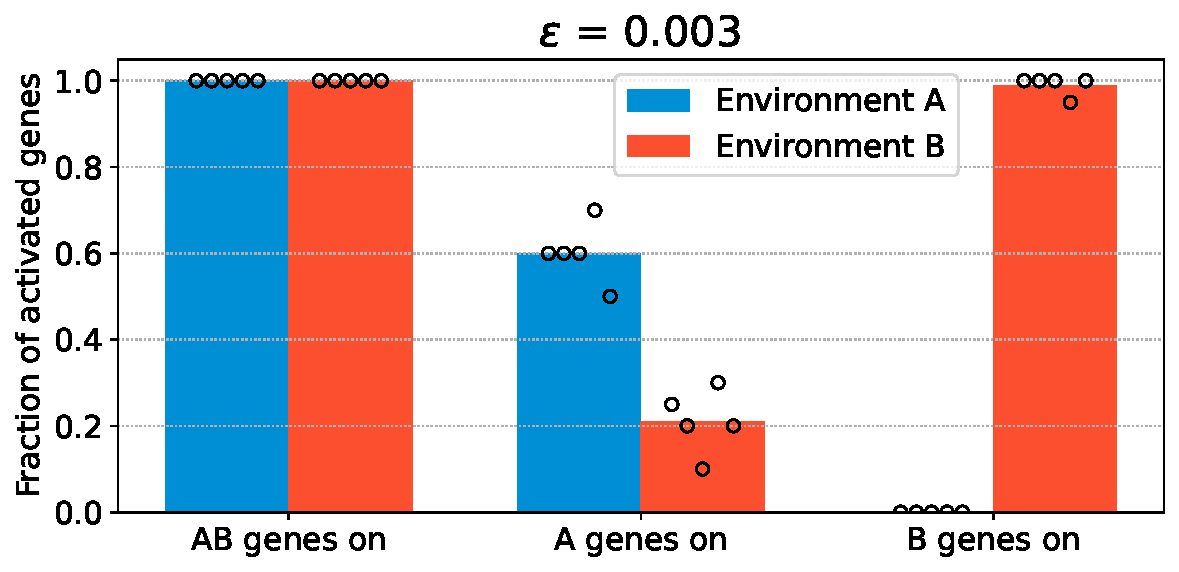
\includegraphics[width=\textwidth]{alife/img/mean_activation_epsilon-0.003.pdf}
\label{subfig:alife:param_epsilon_1}
\end{subfigure}
\begin{subfigure}[t]{0.49\textwidth}
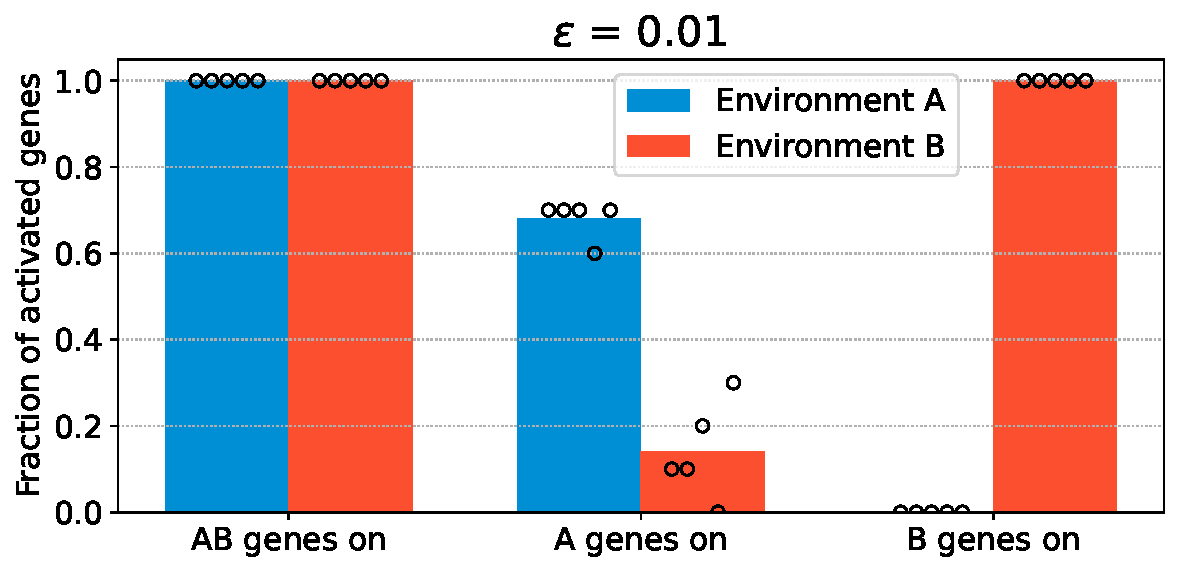
\includegraphics[width=\textwidth]{alife/img/mean_activation_epsilon-0.01.pdf}
\label{subfig:alife:param_epsilon_2}
\end{subfigure}

\begin{subfigure}[t]{0.49\textwidth}
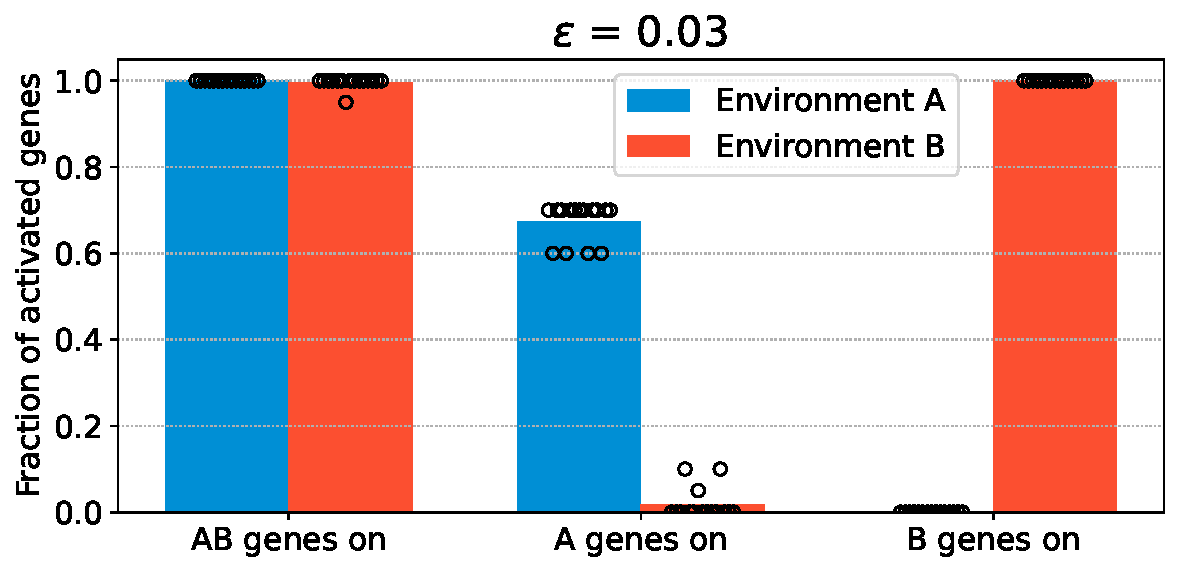
\includegraphics[width=\textwidth]{alife/img/mean_activation_epsilon.pdf}
\label{subfig:alife:param_epsilon_3}
\end{subfigure}
\begin{subfigure}[t]{0.49\textwidth}
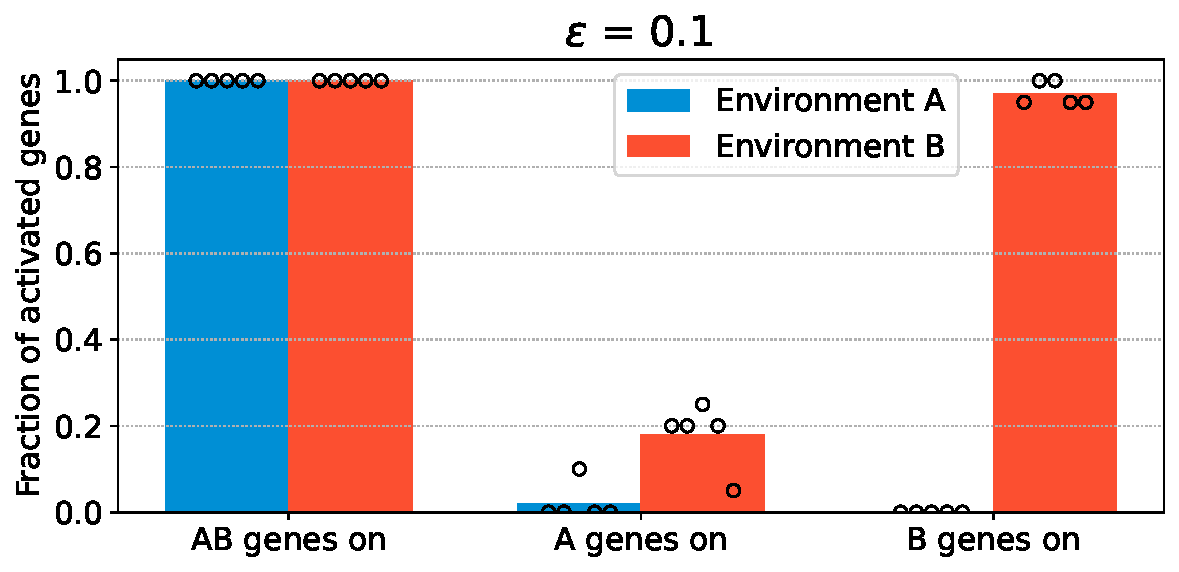
\includegraphics[width=\textwidth]{alife/img/mean_activation_epsilon-0.1.pdf}
\label{subfig:alife:param_epsilon_4}
\end{subfigure}
\caption[Parameter exploration in the proof-of-concept model: varying $\epsilon$]{Average fraction of activated genes in each environment at the end of evolution, for increasing values of $\epsilon$, from top to bottom and left to right.
Every replicate is shown as a dot, and the bottom-left panel ($\epsilon = 0.03$) recalls data from the main run (which has 15 replicates) for comparison.
For all values of $\epsilon$ except $0.1$, the behavior from the main run is qualitatively replicated.}
\label{fig:alife:param_epsilon}
\end{figure}

The results of these additional simulations are presented in figures~\ref{fig:alife:param_epsilon},~\ref{fig:alife:param_c} and~\ref{fig:alife:param_sigma}.
For $\epsilon$, we chose values of $\epsilon = 0.003$, $\epsilon = 0.01$, and $\epsilon = 0.1$, compared to an initial value of $\epsilon = 0.03$, and the results are shown in Figure~\ref{fig:alife:param_epsilon}.
For the values of $\epsilon$ lower than the default (top row), representing a higher sensitivity of promoters to supercoiling, we observe the evolution of differentiated gene expression levels as in the main run (bottom-left panel), whereas for the higher value of $\epsilon$ (bottom-right panel), \emph{A} genes are still not expressed in environment A by the end of evolution.
In this case, promoters are not sensitive enough to the supercoiling variations caused by the transcription-supercoiling coupling, and genes are unable to overcome the highly positive supercoiling of environment A.

\begin{figure}[H]
\centering
\begin{subfigure}[t]{0.49\textwidth}
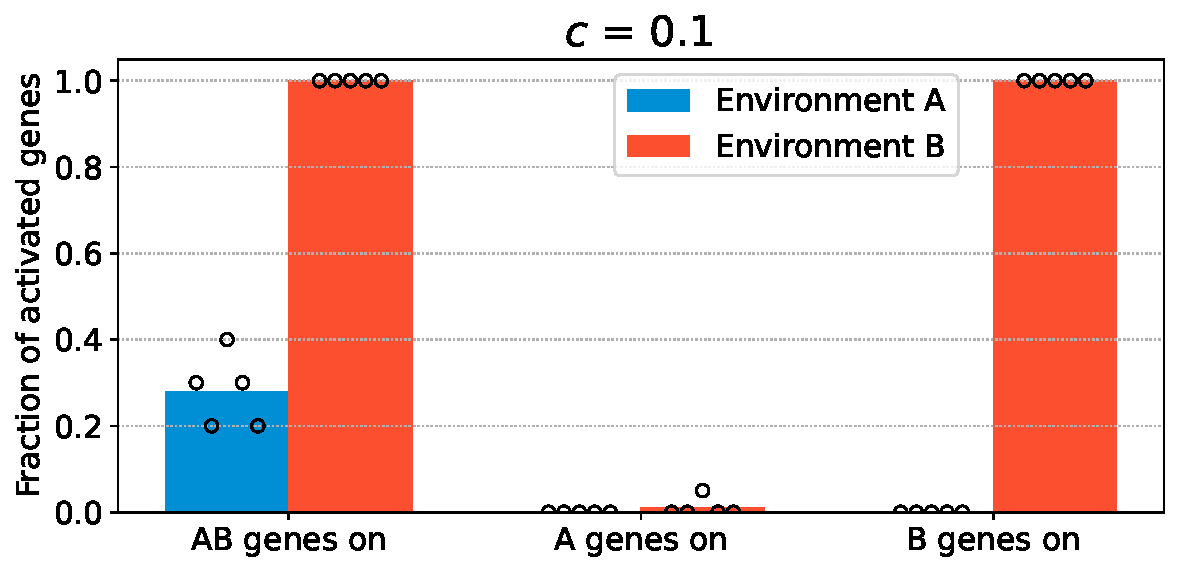
\includegraphics[width=\textwidth]{alife/img/mean_activation_inter-coef-0.1.pdf}
\label{subfig:alife:param_c_1}
\end{subfigure}
\begin{subfigure}[t]{0.49\textwidth}
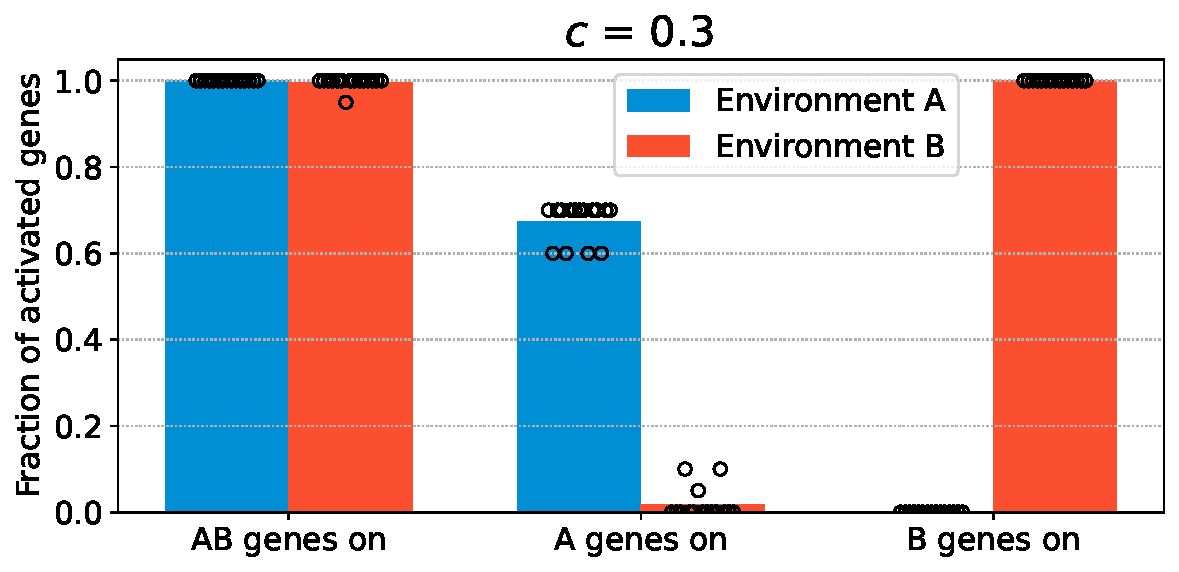
\includegraphics[width=\textwidth]{alife/img/mean_activation_inter_coef.pdf}
\label{subfig:alife:param_c_2}
\end{subfigure}

\begin{subfigure}[t]{0.49\textwidth}
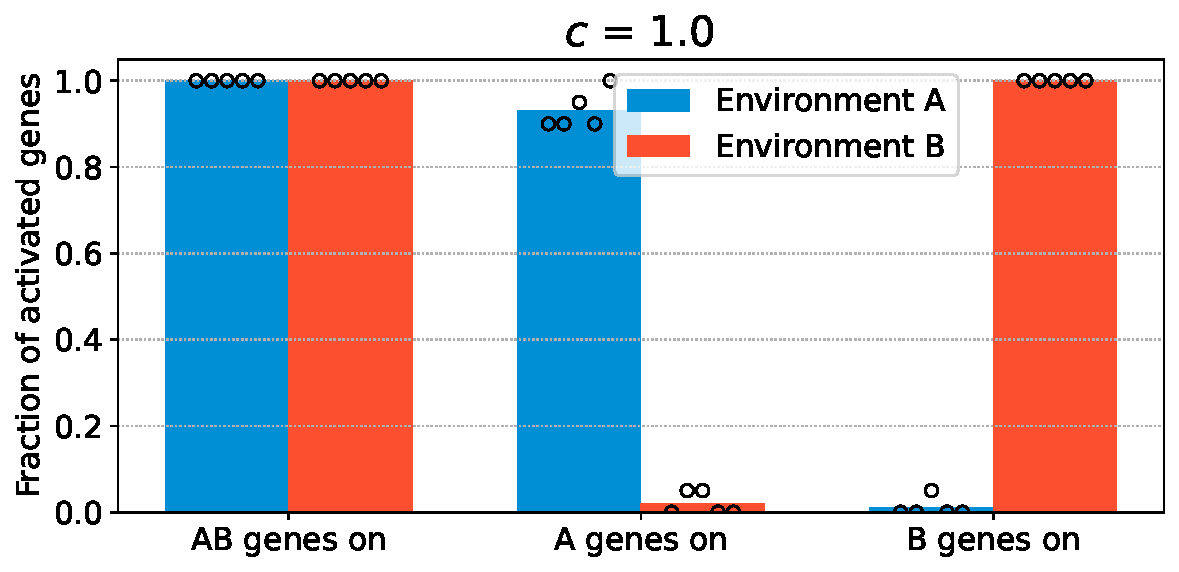
\includegraphics[width=\textwidth]{alife/img/mean_activation_inter-coef-1.0.pdf}
\label{subfig:alife:param_c_3}
\end{subfigure}
\begin{subfigure}[t]{0.49\textwidth}
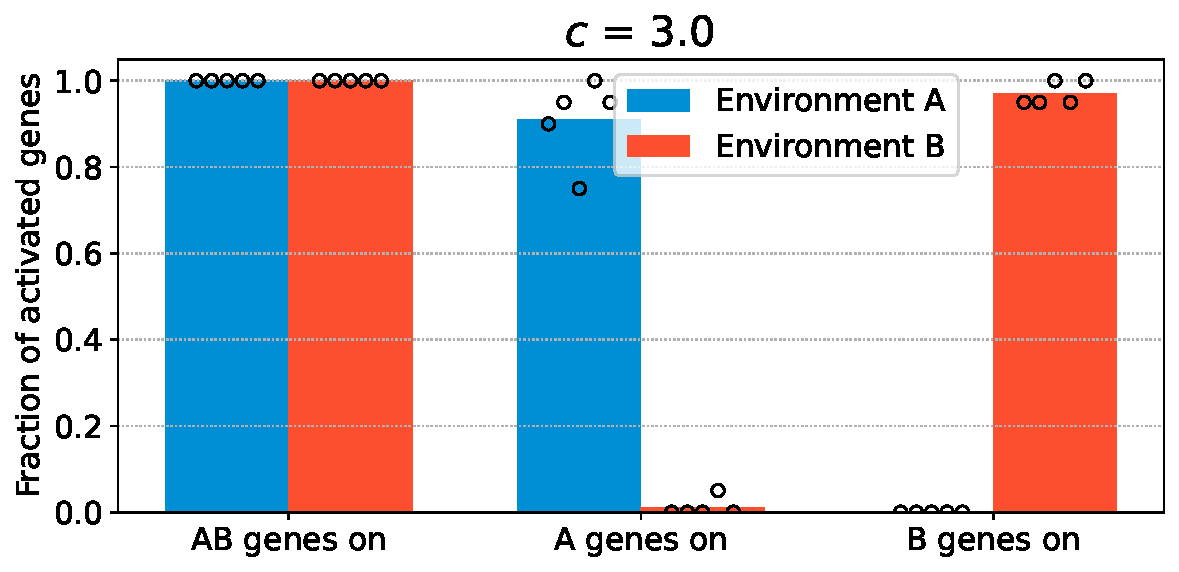
\includegraphics[width=\textwidth]{alife/img/mean_activation_inter-coef-3.0.pdf}
\label{subfig:alife:param_c_4}
\end{subfigure}
\caption[Parameter exploration in the proof-of-concept model: varying $c$]{Average fraction of activated genes in each environment at the end of evolution, for increasing values of $c$, from top to bottom and left to right.
Every replicate is shown as a dot, and the top-right panel ($c = 0.3$) recalls data from the main run for comparison.
For all values of $c$ except $0.1$, the behavior from the main run is qualitatively replicated.}
\label{fig:alife:param_c}
\end{figure}

For $c$, we chose values of $c = 0.1$, $c = 1.0$, and $c = 3.0$, for an initial value of $c = 0.3$, and the results are shown in Figure~\ref{fig:alife:param_c}.
Similarly to $\epsilon$, when $c$ is too low (top-left panel), genes do not interact strongly enough for a differentiated phenotype to evolve as a function of the environment, whereas higher values of $c$ (bottom row) show the same evolutionary behavior as the main run (top-right panel).

\begin{figure}[H]
\begin{subfigure}[t]{0.49\textwidth}
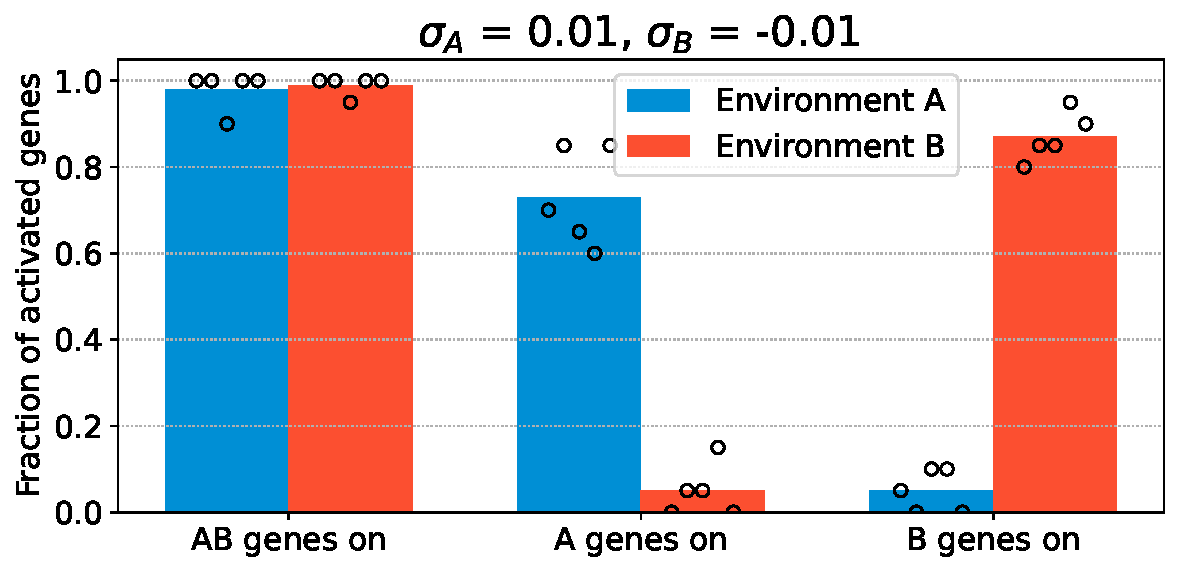
\includegraphics[width=\textwidth]{alife/img/mean_activation_sigma-0.01.pdf}
\label{subfig:alife:param_sigma_1}
\end{subfigure}
\begin{subfigure}[t]{0.49\textwidth}
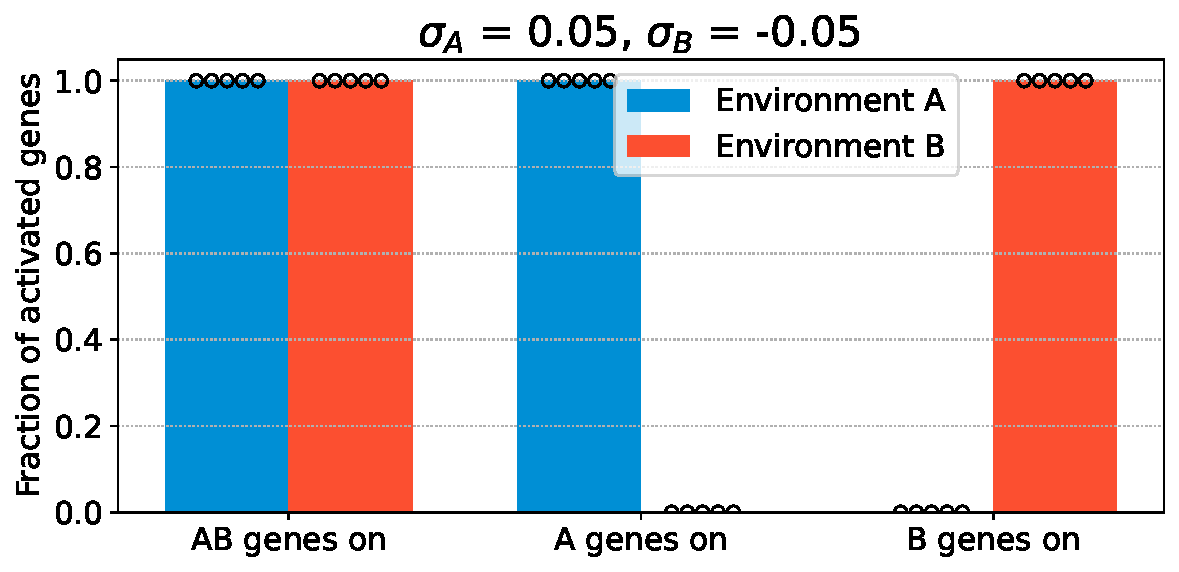
\includegraphics[width=\textwidth]{alife/img/mean_activation_sigma-0.05.pdf}
\label{subfig:alife:param_sigma_2}
\end{subfigure}

\begin{subfigure}[t]{0.49\textwidth}
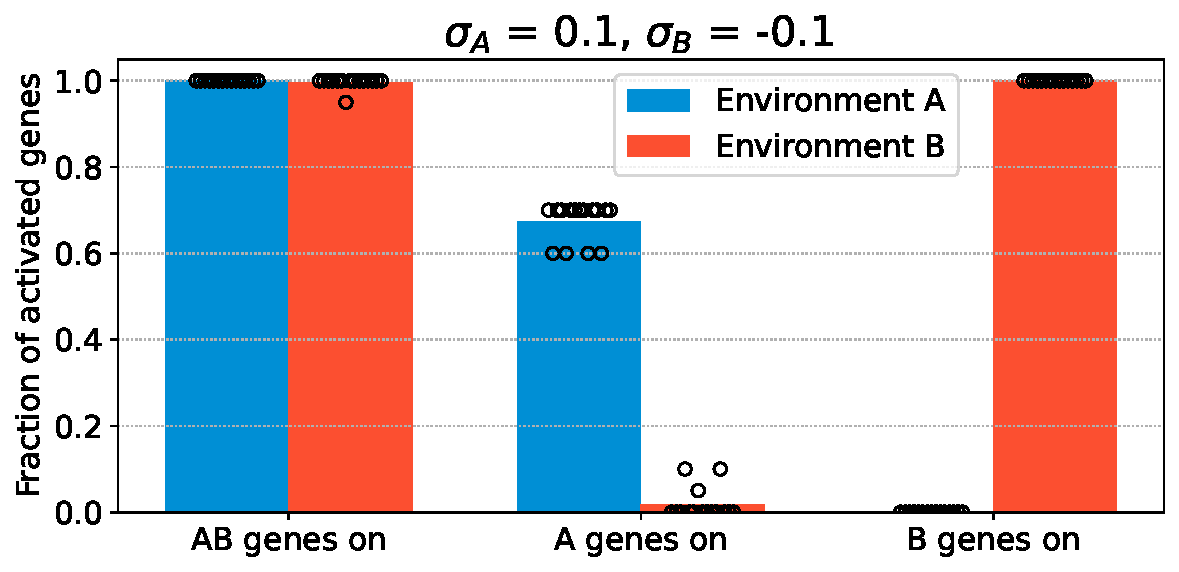
\includegraphics[width=\textwidth]{alife/img/mean_activation_sigma.pdf}
\label{subfig:alife:param_sigma_3}
\end{subfigure}
\begin{subfigure}[t]{0.49\textwidth}
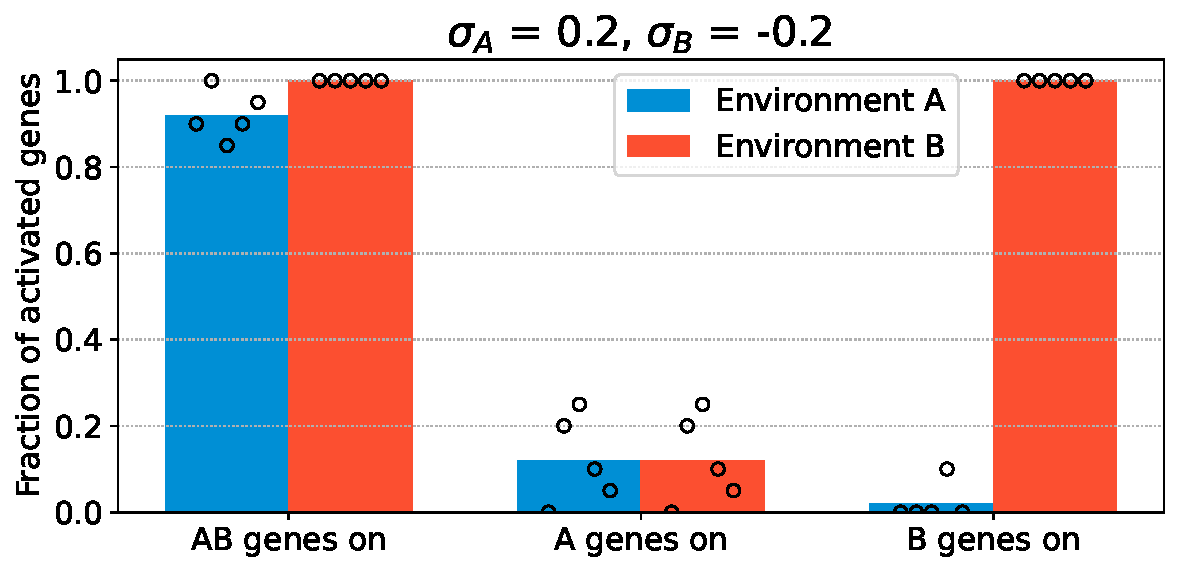
\includegraphics[width=\textwidth]{alife/img/mean_activation_sigma-0.2.pdf}
\label{subfig:alife:param_sigma_4}
\end{subfigure}
\caption[Parameter exploration in the proof-of-concept model: varying $\sigma_A$ and $\sigma_B$]{Average fraction of activated genes in each environment at the end of evolution, for more and more distinct environments $\sigma_A$ and $\sigma_B$, from top to bottom and left to right.
Every replicate is shown as a dot, and the bottom-left panel ($\sigma_A = 0.1$, $\sigma_B = -0.1$) recalls data from the main run for comparison.
For all values except $\sigma_A = 0.2$ and $\sigma_B = -0.2$, the behavior from the main run is qualitatively replicated.}
\label{fig:alife:param_sigma}
\end{figure}

Finally, we also investigate different amplitudes in the difference in supercoiling level between the two environments, by choosing values of $\sigma_A = 0.01$, $\sigma_A = 0.05$ and $\sigma_A = 0.2$, and $\sigma_B = -\sigma_A$ respectively in each case (for an initial value of $\sigma_A = 0.1$ and $\sigma_B = -0.1$).
We observe that, when $\sigma_A = 0.2$ (bottom-right panel), the environmental supercoiling constraint is too high and \emph{A} genes are not activated in environment A by the end of the runs.
However, for environments closer to each other than the default (top row), evolution is able to leverage the differences in supercoiling between these environments to evolve differentiated phenotypes, as in the main run (bottom-left panel), showing that our model remains sensitive to small changes in environmental supercoiling.

To conclude, in our model, the gene interaction network is therefore able to respond to different environments and can evolve an efficient regulation of gene expression under a broad range of parameter values, reinforcing the hypothesis that a supercoiling-mediated coupling between gene expression levels could indeed play a functional role in biological organisms.

\section{Discussion and Perspectives}

DNA supercoiling plays a fundamental role in the regulation of gene transcription in bacteria, and an important part of this role could be mediated by the local variations in supercoiling that are caused by the transcription-supercoiling coupling.
While the influence of the global supercoiling level on gene transcription~\citep{lal2016, ma2016,dorman2016, martisb.2019}, the evolutionary importance of supercoiling regulation~\citep{crozat2005,crozat2010, duprey2021} and the mechanistic details of the transcription-supercoiling coupling~\citep{meyer2014, elhoudaigui2019} have all already been studied, no existing work did to our knowledge tackle the question of the possible role of the transcription-supercoiling coupling both at the whole-genome scale and on an evolutionary time scale.

In this work, we have developed a genome-wide model of the influence of DNA supercoiling on gene transcription, incorporating both the global influence of the environment and the local variations in the supercoiling level that are due to the transcription-supercoiling coupling.
We have shown that, in our model, complex interactions implicating several genes emerge from the coupling between supercoiling and transcription.
Indeed, \emph{A} genes display an activation pattern that would not be obtainable without the network of interactions that results from the coupling.
Thanks to this network, \emph{A} genes are activated in an environment where isolated genes would be inhibited, and inhibited in an environment where isolated genes would be activated.
The transcription-supercoiling coupling therefore enables the selective activation or inhibition of specific sets of genes, providing a non-monotonic response to environmental variations through changes in the level of DNA supercoiling.
Furthermore, we have shown, using an \emph{in silico} experimental evolution approach, that natural selection can leverage this biophysical mechanism to selectively turn on or off several pools of genes, using only the very simple mutation operator of genomic inversions, that affect the relative positions and orientations of genes on the genome but do not change genome length or basal gene transcription rates, and that this behavior is able to evolve under a wide range of parameter values.
This response of gene transcription levels to DNA supercoiling reflects a phenomenon which has been observed \emph{in vivo} in the expression of pathogenicity-related genes in specific environments, such as the normally lethal inside of the macrophage for the mammalian pathogen \emph{S. enterica}~\citep{cameron2013}, or plant tissue for \emph{D. dadantii}~\citep{herault2014}.

Our model voluntarily stays very simple, only incorporating the most important feature of the transcription-supercoiling coupling, which is the non-linear interaction between the expression levels of neighboring genes.
This simplicity therefore hints at the possible pervasiveness of this regulation mechanism throughout the prokaryotic realm.
Nonetheless, in order to go further and represent more accurately the diversity of gene behaviors found in real life, several more dimensions could be integrated to the model.
At present, the target for genes in our model is bistability, meaning that genes should end up fully activated or fully inhibited.
A more biologically plausible approach would be to relax this restriction and give genes arbitrary expression targets, in order to determine to which extent the transcription-supercoiling coupling is able to finely regulate gene expression.
Furthermore, unlike in our model (in which all genes have the same response curve to DNA supercoiling), the genes of biological organisms can show different responses to the supercoiling level.
These differences are partly caused by the GC content at the gene promoter~\citep{forquet2021}, and some genes can even respond in the opposite direction to DNA relaxation, that is to say be activated rather than inhibited by less negatively supercoiled DNA.
This behavior is for instance present in the \emph{gyrA} and \emph{gyrB} genes that encode the gyrase subunits in \emph{E. coli}~\citep{peter2004}.
Moreover, while our model studies its role in an abstract transcription model, supercoiling intervenes during different parts of the initiation and termination of transcription, as well as in in transcript elongation~\citep{martisb.2019}.
Incorporating such precise mechanistic processes into our model could give more accurate information on the link between the position of genes on the genome and their transcription rate.
Similarly, increasing the number of genes of individuals in our model to match bacterial gene numbers might provide more fine-grained results, but is computationally intractable in the current implementation of the model.
Furthermore, investigating the behaviors of individuals when they are placed successively in different environments, rather than evaluated separately in each environment, would also bring more information on the plasticity of the network of gene interaction levels that emerges from the transcription-supercoiling coupling.
Finally, another valuable approach in order to bring this model closer to biology would be to incorporate it into a larger existing framework, such as the Aevol \emph{in silico} experimental evolution platform~\citep{rutten2019}, which models the bacterial genome in much more detail, in order to leverage the power of a well-understood digital organism model.

\chapter{PLOS CB Paper}
\label{chap:ploscb}

\section{Background}

DNA, the material basis of genetic information, is a flexible polymer comprising two strands of nucleotides that coil around each other, at a rate of 10.5 base pairs per turn.
When subjected to torsional stress, DNA can either writhe and form 3-dimensional loops, or twist around itself more or less tightly than in its relaxed state~\citep{travers2005}; both forms are referred to as DNA supercoiling, which is measured as the relative density of supercoils $\sigma$ compared to relaxed DNA.
DNA is positively supercoiled ($\sigma > 0$) when it is overwound, and negatively supercoiled ($\sigma < 0$) when it is underwound.
In bacteria, DNA is normally maintained in a moderately negatively supercoiled state, with a reference value of $\sigma=-0.06$ in \emph{Escherichia coli}~\citep{travers2005}.
DNA supercoiling plays an important role in the regulation of gene expression in bacteria~\citep{martisb.2019}, as it is highly dynamic, and varies in both space along the chromosome and time during the cell lifecycle~\citep{krogh2018}, and as the level of supercoiling at the promoter of a gene modulates the expression of that gene~\citep{forquet2021}.
Furthermore, gene transcription itself locally impacts the level of DNA supercoiling, resulting in an interplay between the supercoiling and transcription of neighboring genes~\citep{meyer2014}, which hints at a possible role for this coupling as an evolutionary force shaping genome organization~\citep{junier2016}.

\subsection{The Dynamic Nature of DNA Supercoiling}

The level of DNA supercoiling in bacteria is controlled by topoisomerases, enzymes that alter DNA supercoiling by cutting and rotating the DNA strands~\citep{duprey2021}; the two main topoisomerases being gyrase, which dissipates positive supercoiling by introducing negative supercoils at an ATP-dependent rate, and topoisomerase I, which oppositely relaxes negative supercoiling~\citep{martisb.2019}.
Many other processes however influence the level of DNA supercoiling.
According to the twin-domain of supercoiling~\citep{liu1987}, the transcription of a gene by RNA polymerase generates a buildup of positive supercoiling upstream of the gene, and negative supercoiling downstream of the gene, through the rotational drag that hampers the rotation of the polymerase around DNA.
At a larger scale, while the intrinsic flexibility of the DNA polymer would allow supercoils to propagate freely along its length, many nucleoid-associated proteins such as FIS, H-NS or HU bind to bacterial DNA (in addition to RNA polymerases), and create topological barriers that instead block the diffusion of supercoiling~\citep{travers2005}.
In bacteria, the level of DNA supercoiling can furthermore be affected by numerous environmental challenges.
Salt shock transiently increases negative DNA supercoiling in \emph{E. coli}~\citep{hsieh1991}; the acidic intracellular environment relaxes DNA in the facultative pathogen \emph{Salmonella enterica} var. Typhimurium~\citep{marshall2000}; and higher temperatures relax DNA in the plant pathogen \emph{Dickeya dadantii}~\citep{herault2014}.
These constraints overall result in a very dynamic DNA ``supercoiling landscape'' in \emph{E. coli}~\citep{visser2022}, with a supercoiling level that varies in both time during the bacterial lifecycle and space along the chromosome.
%, but increases negative supercoiling in the human pathogen \emph{Shigella flexneri}~\citep{tobe1995}. % Note: at the promoter of _virB_ yes, but not genome-wide

\subsection{DNA Supercoiling and Gene Regulation}

Many bacteria leverage the regulating effect of DNA supercoiling on gene transcription by modulating their DNA supercoiling level.
In several bacteria such as \emph{E. coli}, \emph{S. enterica}, or \emph{D. dadantii}, between 5\% and 15\% of genes were found to be sensitive to relaxation or hypercoiling of chromosomal DNA, with genes being up-regulated or down-regulated in each condition~\citep{peter2004, ferrandiz2010, webber2013, pineau2022a}.
DNA supercoiling might in particular be an especially important regulator of gene activity in bacteria with reduced genomes, such as the obligate aphid endosymbiotic bacterium \emph{Buchnera aphidicola}, which is nearly devoid of transcription factors~\citep{brinza2013}.

Moreover, selection can act on the level of DNA supercoiling in order to modulate the regulation of gene expression.
In 10 of the 12 populations in the Long-Term Evolution Experiment (LTEE), an increase in fitness was linked to mutations in the \emph{topA} and \emph{fis} genes, which participate in the regulation of the supercoiling level~\citep{crozat2010}.
When inserted into the ancestral strain, these mutations increased the level of negative supercoiling as well as the bacterial growth rate~\citep{crozat2005}, demonstrating that the level of DNA supercoiling can evolve as part of a regulatory response to new environments.

Finally, the regulation of gene expression by DNA supercoiling could be a force that participates in shaping the evolution of bacterial genomes themselves.
Indeed, supercoiling-sensitive genes tend to group in up or down-regulated clusters in \emph{E. coli}~\citep{peter2004}, \emph{S. enterica}~\citep{webber2013} and \emph{S. pneumoniae}~\citep{ferrandiz2010}, suggesting the possibility of an adaptive role in the co-localization of these clusters.
Indeed, synteny segments, or clusters of neighboring genes that show correlated expression patterns, are evolutionarily conserved across \emph{E. coli} and the distantly related \emph{Bacillus subtilis}~\citep{junier2016}, strengthening the hypothesis that these domains could play an important role in the regulation of bacterial gene expression.

\subsection{The Transcription-Supercoiling Coupling}

As we saw before, the process of transcribing a given gene generates an accumulation of positive supercoiling downstream of that gene, and of negative supercoiling upstream of that gene~\citep{liu1987}.
If a second gene is located closely enough to this first gene, the change in supercoiling at the promoter of the second gene will impact its transcription rate, as negative supercoiling usually facilitates promoter opening, and hence gene transcription~\citep{forquet2021}.
In turn, the second gene will also generate a change in supercoiling that affects the first gene, resulting in an interaction between the transcription levels of these two genes.
Depending on the relative orientation of these genes, several types of interactions are therefore possible: divergent genes reinforce their respective transcription level in a positive feedback loop, convergent genes inhibit the transcription of one another, and for tandem genes, the downstream gene up-regulates the upstream gene, while the upstream gene down-regulates the downstream gene.

This effect, which has been called the transcription-supercoiling coupling~\citep{meyer2014,sobetzko2016,elhoudaigui2019}, has been documented in several bacterial genetic systems.
In \emph{S. flexneri}, the \emph{virB} promoter is normally only active at high temperature, but can be activated at low temperature by the insertion of a phage promoter in divergent orientation~\citep{tobe1995}.
Similarly, the expression of the \emph{leu-500} promoter in \emph{S. enterica} can be increased or decreased by the insertion of upstream transcriptionally active promoters, depending on their orientation relative to \emph{leu-500}~\citep{elhanafi2000}.
The magnitude of this effect has also been explored in a synthetic construct that uses the inducible \emph{ilvY} and \emph{ilvC} \emph{E. coli} promoters, inserted on a plasmid in divergent orientations.
In this system, a decrease in the activity of \emph{ilvY} is associated with a decrease in \emph{ilvC} activity, and an increase in \emph{ilvY} activity with an increase in \emph{ilvC} activity as well~\citep{rhee1999}.

There are, however, hints that the biological relevance of the transcription-supercoiling coupling might not be confined to a few specific cases.
Indeed, in \emph{E. coli}, the typical size of topological domains, inside which the supercoiling generated by gene transcription can propagate, is usually around 10kb~\citep{postow2004}, and could reach up to 25kb~\citep{visser2022} in each direction.
As the average size of \emph{E. coli} genes is 1kb, and the average intergenic distance about 120bp~\citep{blattner1997}, this means that any single topological domain encompasses several genes that can potentially interact via the transcription-supercoiling coupling.
A statistical analysis of the relative position of neighboring genes on the \emph{E. coli} chromosome furthermore shows that genes that are up-regulated by negative supercoiling have more neighbors in divergent orientations, while genes that are down-regulated by negative supercoiling have more neighbors in converging orientations~\citep{sobetzko2016}, suggesting that the transcription-supercoiling coupling plays a role in regulating the activity of these genes.

\paragraph{}
In this article, we present a two-level individual-based model of gene expression at the whole-genome scale, in which gene transcription is regulated solely by DNA supercoiling, and in which populations of individuals evolve towards environment-specific gene expression targets through genomic rearrangements only.
Rather than attempting to give quantitative predictions of the  effect of the transcription-supercoiling coupling on the expression levels of genes in a given, static genetic system, our model aims at exploring the range of genomic organizations that can be generated by selection in order to regulate gene expression levels in different environments through the transcription-supercoiling coupling.
Using this model, we observe the emergence of complex environment-driven patterns of gene expression, and characterize the spatial organization of genes along the genome that underlie these patterns.
We first show that genes are locally organized in convergent or divergent pairs that leverage the transcription-supercoiling coupling to activate or inhibit one another.
Then, we show that this local organization is not entirely sufficient to fully account for the complex gene expression patterns that we observe, but that gene inhibition requires the interaction of a large number of genes.
Finally, we show that, in our model, genes form a dense genome-wide regulatory network, providing insight into the organization of bacterial genomes.


\section{An Evolutionary Model of the Transcription-Supercoiling Coupling}
\label{sec:ploscb:model}

\subsection{Individual-Level Model}
\label{sec:ploscb:indiv_model}

We define the genotype of an individual in our model as a single circular chromosome that is representative of a bacterial chromosome.
The chromosome consists in a fixed number of protein-coding genes, which are separated by non-coding intergenic segments of varying sizes, and has a basal supercoiling level $\sigma_{basal}$.
Each gene on the chromosome is characterized by its starting position (genes cannot overlap in our model), its orientation (on the forward strand or on the reverse strand), its length, and its basal expression level.
We define an environment by the shift $\delta\sigma_{env}$ that it imposes to the supercoiling level of the chromosome.
We then define the phenotype of an individual in a given environment as the gene expression levels that are solution of the system given by the interaction of its genes through the transcription-supercoiling coupling (described below), on a chromosome with a background supercoiling level of $\sigma_{basal} + \delta\sigma_{env}$.

\begin{figure}[H]
  \centering
  \begin{subfigure}[t]{0.44\textwidth}
    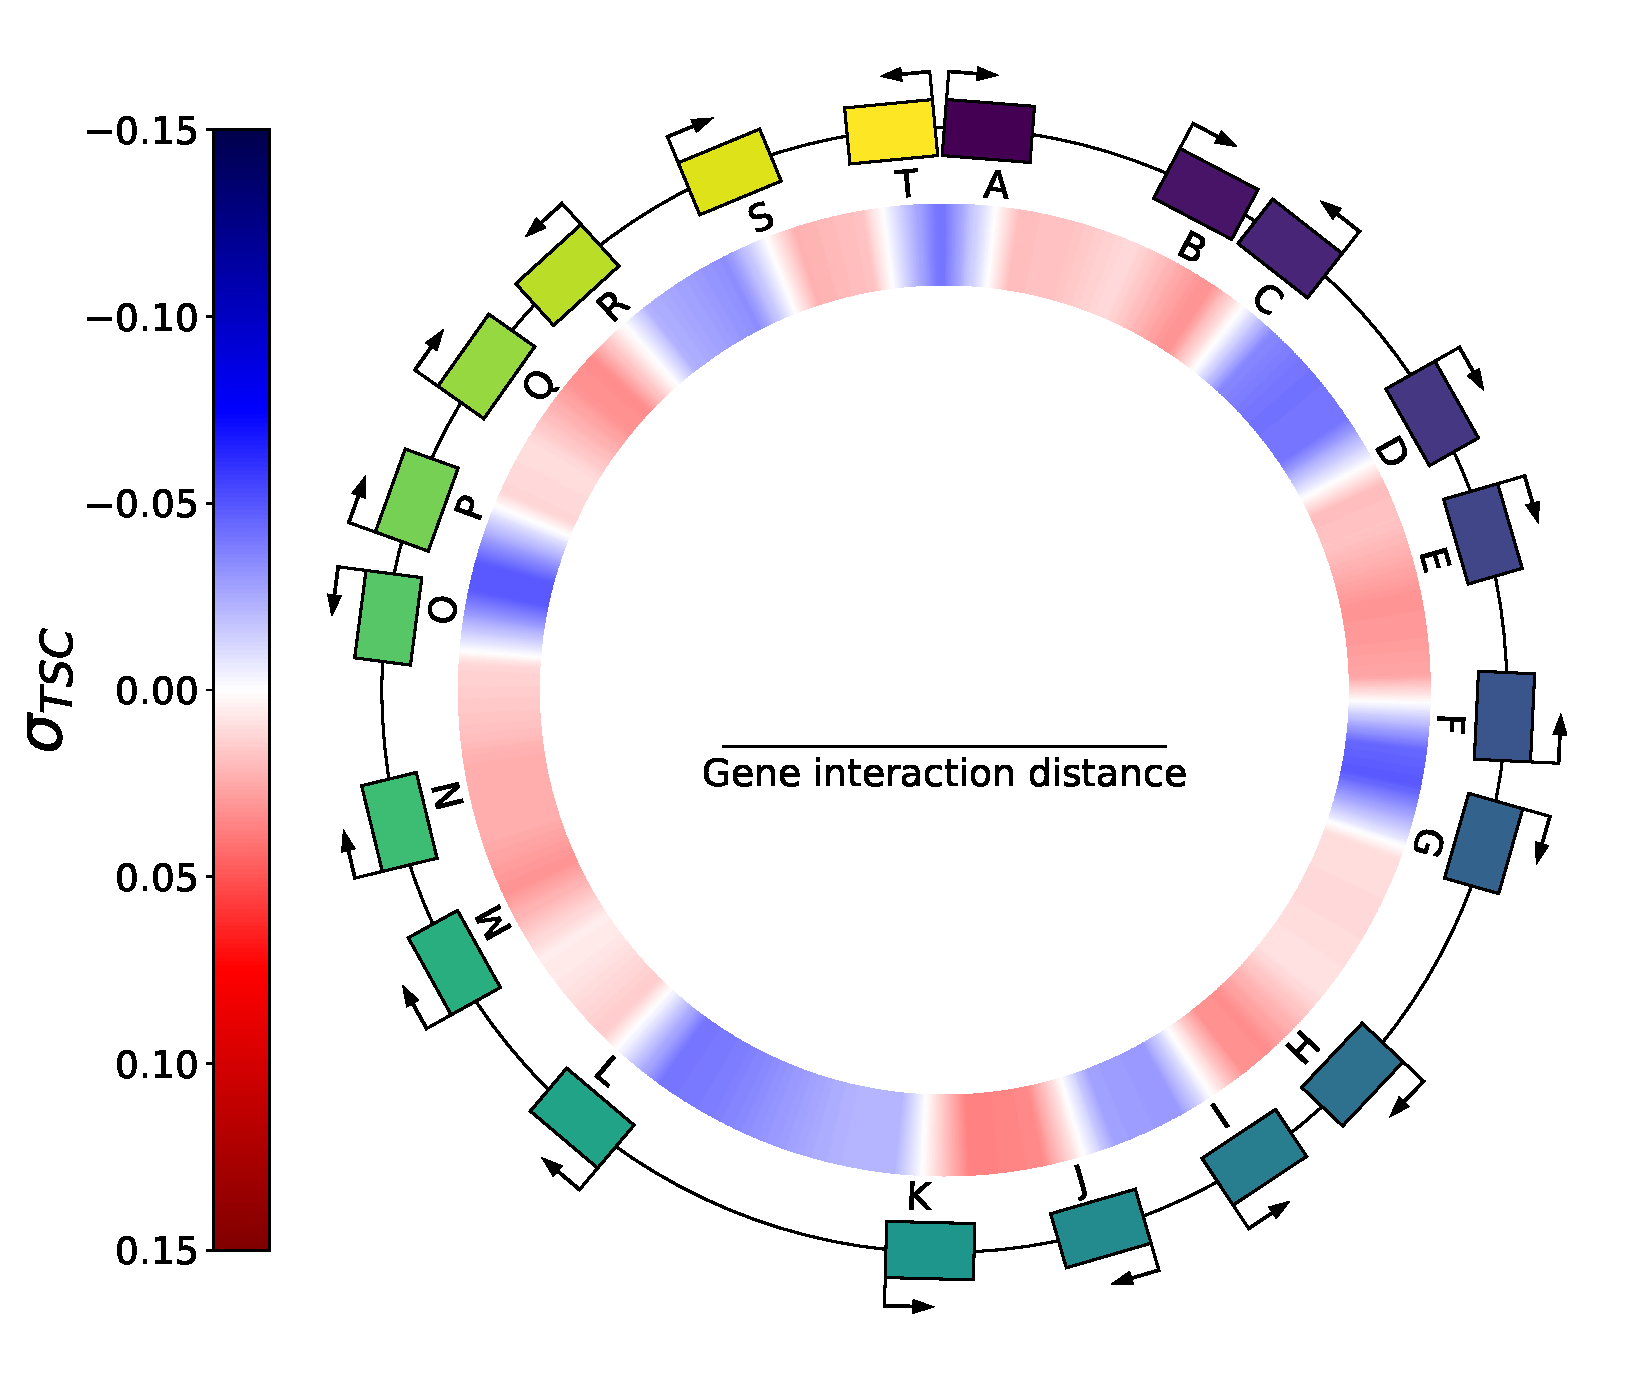
\includegraphics[width=\textwidth]{ploscb/img/random_genome_and_tsc.pdf}
    \label{subfig:ploscb:random_genome}
  \end{subfigure}
  \begin{subfigure}[t]{0.55\textwidth}
    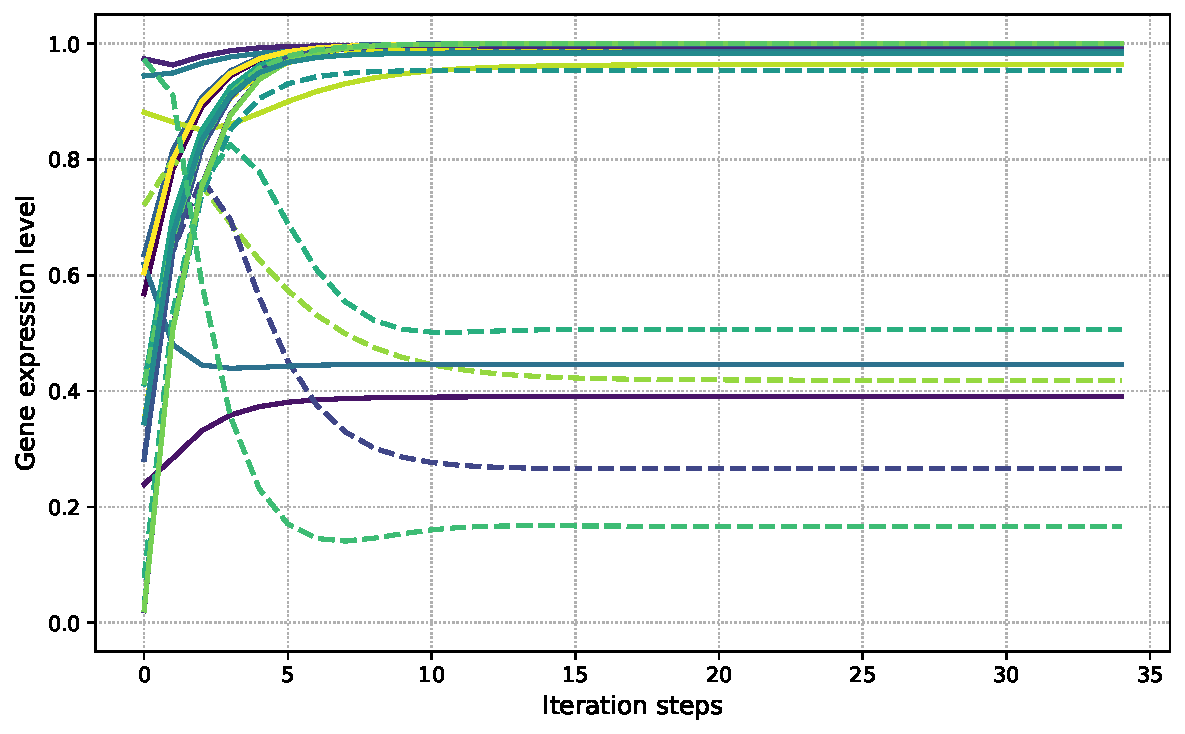
\includegraphics[width=\textwidth]{ploscb/img/random_gene_expr.pdf}
    \label{subfig:ploscb:random_expr}
  \end{subfigure}
  \caption[Example individual in the advanced model, evaluated in both environments]{Left: genome (outer ring) and level of supercoiling generated by transcription ($\sigma_{TSC}$, inner ring) of an example genome with 20 genes placed at random positions and orientations and colored by position, with a gene length and average intergenic distance of 1 kb each, and a basal supercoiling level of $\sigma_{basal} = -0.066$.
  The individual is evaluated in an environment in which $\delta\sigma_{env} = 0$.
  Right: evolution of the expression level of each gene of the individual during the computation of the solution to the system given by equations~\ref{eq:sigma},~\ref{eq:prom_energy}, and~\ref{eq:gene_activity}, starting from random initial values.
  Solid lines represent genes on the forward strand, dashed lines genes on the reverse strand, and gene colors are the same as on the genome.}
  \label{fig:ploscb:random_indiv}
\end{figure}

The genome of an example individual with 20 genes and a basal supercoiling $\sigma_{basal} = -0.066$ is shown on the left-hand side of Figure~\ref{fig:ploscb:random_indiv}.
Inside the genome is the resulting local level of DNA supercoiling when this individual is evaluated in an environment with a supercoiling shift of $\delta\sigma_{env}~=~0$.
As expected given the twin-domain model of supercoiling, we can observe a buildup in negative supercoiling (blue) between genes in divergent orientations, such as genes C and D or F and G, and a buildup in positive supercoiling (red) between genes in convergent orientations, such as genes J and K or Q and R.
The right-hand side panel of Figure~\ref{fig:ploscb:random_indiv} shows the computation of the stable state of gene expression levels for this individual.
Note that, in this model and throughout this article, we conflate
gene transcription rates with mRNA concentrations, as we assume that mRNAs degrade at a constant rate, and as transcription rates in our model are only affected by the effect of supercoiling on transcription.
We furthermore conflate transcription rates with expression levels, as we again assume proteins to be translated at a rate proportional to the associated mRNA concentrations and to degrade at a constant rate.

\paragraph{Effect of Transcription on Supercoiling}
For an individual with a genome containing $n$ genes, each expressed at a level $e_i$, we model the influence of the transcription of each gene on the level of supercoiling at the promoter of every other gene in the form of an $n$-by-$n$ interaction matrix.
The coefficient $\frac{\partial\sigma_i}{\partial e_j}$ at indices $(i, j)$ in this matrix represents the variation in DNA supercoiling at the promoter of gene $i$ due to the transcription of gene $j$.
The value of this coefficient is given by the following formula:

\begin{equation}
  \frac{\partial\sigma_{i}}{\partial e_j} = \eta \cdot c \cdot \max(1-\frac{d(i, j)}{d_{max}}, 0)
  \label{eq:dsigmade}
\end{equation}

$\eta$ represents the sign of the interaction, which depends on the position and orientation of gene $j$ relative to gene $i$, according to the twin-domain model.
If gene $j$ is upstream of gene $i$, and if it is on the same strand as (or points towards) gene $i$, then its transcription generates a buildup in positive supercoiling at gene $i$ ($\eta = 1$).
Conversely, if gene $j$ is upstream of gene $i$ but on the other strand than (or points away from) gene $i$, it generates a buildup in negative supercoiling at gene $i$ ($\eta = -1$).
If gene $j$ is instead located downstream of gene $i$, the sign of the interaction in each case is switched: $\eta = 1$ if the genes are on the same strand, and $\eta = -1$ otherwise.

We then apply a scaling coefficient $c$, which represents the intensity to which the transcription-generated torsion of DNA affects the local level of supercoiling.
Finally, the strength of the interaction decreases linearly with the distance $d(i, j)$ between the promoter of gene $i$, which is the position where the local level of supercoiling affects the probability that an RNA polymerase binds to the DNA and starts transcribing gene $i$, and the middle of gene $j$, which is the average location of the RNA polymerases that transcribe gene $j$, assuming that DNA is transcribed at a constant speed.
When this distance reaches a threshold of $d_{max}$, the two genes are considered to be too far away to interact and the effect vanishes.

\paragraph{Effect of Supercoiling on Transcription}
In order to compute the transcription level of a given gene, we first compute the opening free energy of its promoter, which depends on the local supercoiling level, following a sigmoidal curve that increases with negative supercoiling until a saturation threshold is reached~\citep{forquet2021}.
In order to model this effect, we adapted the equations and parameter values presented in~\cite{elhoudaigui2019}, which are based on the \emph{in vitro} analysis of the transcription of model bacterial promoters.
We first compute the local level of supercoiling $\sigma_i$ at the promoter of gene $i$, which is the sum of the background supercoiling level $\sigma_{basal} + \delta\sigma_{env}$ (which is constant along the genome for any given individual), and of the local variation in supercoiling caused by the transcription of every other gene (represented in Figure~\ref{fig:ploscb:random_indiv} as $\sigma_{TSC}$):

\begin{equation}
  \sigma_i = \sigma_{basal} + \delta\sigma_{env} + \sum_{j=1}^n\frac{\partial\sigma_{i}}{\partial e_j}e_j
  \label{eq:sigma}
\end{equation}

We compute the expression level of the gene using a thermodynamic model of transcription.
First, we compute the opening free energy $U_i$ of the promoter of gene $i$, which depends on $\sigma_i$, the level of supercoiling at the promoter and on $\sigma_0$, the level of supercoiling at which the opening free energy is at half its maximum level, according to the following sigmoidal function:

\begin{equation}
  U_i = \frac{1}{1 + e^{(\sigma_i - \sigma_0)/\epsilon}}
  \label{eq:prom_energy}
\end{equation}

The, we compute the expression level $e_i$ of gene $i$ using the promoter opening free energy, with a scaling constant $m$:

\begin{equation}
  e_i = e^{m (U_i - 1)}
  \label{eq:gene_activity}
\end{equation}

The transcription level of a gene is therefore expressed in arbitrary units between $e^{-m}$, the minimum expression level when the promoter is most hindered by supercoiling (when $U_i$ = 0), and 1, the maximum expression level, when the promoter is most activated by supercoiling (when $U_i$ = 1).
Throughout this manuscript, we will describe a gene as activated if its transcription level is above the mean of these two values $e_{1/2} = \frac{1}{2}(e^{-m} + 1)$, and inhibited otherwise.

\paragraph{Computation of Gene Expression Levels}

We define the phenotype of an individual in an environment (described by $\delta\sigma_{env}$) as the set of gene expression levels that is solution to the system given by equations~\ref{eq:sigma},~\ref{eq:prom_energy} and~\ref{eq:gene_activity}, in that environment.
In order to compute this phenotype, we numerically compute a solution to the system of equations using a fixed-point iteration algorithm, and starting from an initial state in which all genes are expressed at $e_{1/2}$.
A representative example of this computation can be found in Figure~\ref{fig:ploscb:random_indiv}: After an initially unstable phase, the algorithm quickly converges to a fixed point of expression levels.

\subsection{Evolutionary Model}
\label{sec:ploscb:evol_model}

Equipped with a model of the coupling between DNA supercoiling and gene transcription at the whole-genome scale, we now extend it into an evolutionary framework.
In order to study the transcriptional response of individuals placed in different environments, we model the evolution of a population of individuals, each behaving as described in subsection~\ref{sec:ploscb:indiv_model}, in two distinct environments named A and B.
Environment A is a DNA relaxation-inducing environment, with a supercoiling shift of $\delta\sigma_{env} = \delta\sigma_A > 0$, and environment B is a DNA hypercoiling-inducing environment, with a supercoiling shift of $\delta\sigma_{env} = \delta\sigma_B < 0$.
We then define three classes of genes with environment-specific target expression levels: \emph{AB} genes should be expressed in both environments, akin to housekeeping genes; \emph{A} genes should be expressed in environment A but not in environment B; and, conversely, \emph{B} genes should be expressed in environment B but not in environment A; both classes represent environment-specific genes such as the pathogenic genes of \emph{S. enterica} or \emph{D. dadantii}~\citep{cameron2012,herault2014}.

\paragraph{Fitness}
Let $(e^A_A, e^A_B, e^A_{AB})$ be the average gene expression level per gene type of an individual with $n$ genes in environment A, $(e^B_A, e^B_B, e^B_{AB})$ the average gene expression per type in environment B, and $(\tilde{e}^A_A, \tilde{e}^A_B, \tilde{e}^A_{AB})$ and $(\tilde{e}^B_A, \tilde{e}^B_B, \tilde{e}^B_{AB})$ be target expression values for each gene type in each environment.
For environment A, we choose to set $\tilde{e}^A_A = \tilde{e}^A_{AB} = 1$, and $\tilde{e}^A_B = e^{-m}$, which are respectively the maximal and minimal attainable gene expression levels in the model.
Similarly, for environment B, we set $\tilde{e}^B_B = \tilde{e}^B_{AB} = 1$, and $\tilde{e}^B_A = e^{-m}$.
We then compute the sum $g$ of the squared error between the mean and targeted expression levels for each gene type in each environment:

\begin{equation}
  g = \sum_{i\in\{A, B, AB\}}\left(e^A_i - \tilde{e}^A_i\right)^2 + \sum_{i\in\{A, B, AB\}}\left(e^B_i - \tilde{e}^B_i\right)^2
  \label{eq:gap}
\end{equation}

Finally, we define the fitness of the individual as $f = \exp(-k \cdot g)$, where $k$ is a scaling factor representing the intensity of selection: as $k$ increases, the difference in fitness, and hence in reproductive success, between individuals with different values of $g$ also increases.

\paragraph{Generational Evolutionary Algorithm}
At each generation, we compute the fitness of each individual, by computing their gene transcription levels in each environment, as previously described.
In order to create the next generation, we choose a parent from the current population for each individual in the new population, with a probability proportional to the fitness of the parent.
Then, we create the genome of the new individual by stochastically applying mutations to the genome of its parent.

\paragraph{Mutational Operator: Genomic Inversions}
As this work aims at studying genome organization, we chose to use genomic inversions as the only mutational operator, so that genes can be reordered on the chromosome through evolutionary time; note that other genomic rearrangements, such as translocations, can be modeled as a series of well-chosen consecutive inversions, and are therefore implicitly present in our model.

In order to perform a genomic inversion, we choose a start point and an end point uniformly at random, in the non-coding intergenic sections.
This ensures that genes cannot be broken apart by inversions, as we assume that gene losses are lethal and therefore never conserved.
Having chosen the ends of the inversion, we extract the DNA segment between these ends and insert it in the reverse orientation.
The inversion therefore switches the orientation of every gene inside the segment, but conserves the relative positions and distances of these genes.
Note that, contrary to the intergenic sections that are inside of the inversion, the intergenic sections that are at its boundaries change according to the position of the start and end points of the inversion, allowing the distances between genes to change over evolutionary time.

When mutating an individual, we first draw a number of inversions to perform from a Poisson law of parameter $\lambda = 2$, meaning that the offspring of the individual will on average undergo two inversions, and then perform each inversion in succession to obtain the final mutated offspring.


\section{Results}

In this section, we first show that, as in the proof-of-concept model presented in~\citep{grohens2021}, populations of individuals in the model presented in Section~\ref{sec:ploscb:model} evolve gene expression levels that match their targets in each environment.
Then, we show that, consistently with the theoretical expectations of the twin-domain model, the genomes of evolved individuals are enriched in pairs of divergent or convergent genes that leverage the transcription-supercoiling coupling to regulate gene expression.
Finally, we show that the gene regulatory network generated by the transcription-supercoiling coupling cannot simply be recapitulated by these local interactions, but rather encompasses the whole genome.

\subsection{Experimental Setup}

We evolved 30 populations of 100 individuals, each starting from clones of a random individual with 60 genes (20 of each type), for 1,000,000 generations.
The parameter values that we used are given in Table~\ref{tab:param_values}, and can be broadly grouped into genome-level parameters (gene length, intergenic distance, basal supercoiling level and supercoiling transmission distance) and promoter-level parameters (promoter opening threshold and energy, crossover width).
Both the genome-level parameters that describe the chromosome and the promoter-level parameters used to compute the transcriptional response to supercoiling were taken from experimental values measured in \emph{E. coli}.
In our model, we introduced the torsional drag coefficient as a new parameter that represents the influence of torsional drag on the local level of supercoiling, and empirically chose its value so that this effect is of the same magnitude as that of the other sources of supercoiling variations.

\begin{table}[H]
  \begin{center}
    \begin{tabular}{ l  l  r  c }
    \toprule
    \textbf{Parameter} & \textbf{Symbol} & \textbf{Value} & \textbf{Reference} \\
    \midrule
    %Population size & $N$ & 100 & \\
    %Number of genes & $n$ & 60 \\
    Gene length & $l$ & 1,000 bp & \cite{blattner1997} \\
    Initial intergenic distance & $d_0$ & 125 bp & \cite{blattner1997} \\
    Supercoiling transmission distance & $d_{max}$ & 5,000 bp & \cite{klein2021} \\
    Basal supercoiling level & $\sigma_{basal}$ & -0.066 & \cite{crozat2005} \\
    \midrule
    Torsional drag coefficient & $c$ & 0.03 & \\
    \midrule
    Promoter opening threshold & $\sigma_{opt}$ & -0.042 & \cite{elhoudaigui2019} \\
    Inverse promoter opening energy & $m$ & 2.5 & \cite{elhoudaigui2019} \\
    Crossover width & $\epsilon$ & 0.005 & \cite{elhoudaigui2019} \\
    \bottomrule
    \end{tabular}
    \end{center}
  \caption[Table of parameter values used for the advanced \emph{EvoTSC} runs]{Table of parameter values used in the evolutionary runs.
  The upper set of parameters is the genome-level parameters, the lower set the promoter-level parameters, both taken from the \emph{E. coli} literature; the middle parameter is a new addition from our model.}
  \label{tab:param_values}
\end{table}

The simulation was implemented in Python, with computationally heavy parts optimized using the \texttt{numba} package~\citep{lam2015}. The source code for the simulation, as well as the data analysis code, are available online at \url{https://gitlab.inria.fr/tgrohens/evotsc}.
Running the complete simulation took around 36 hours of computation on a server using a 24-core Intel Xeon E5-2620 v3 @ 2.40GHz CPU, with each replicate running on a single core and using approximately 300 MB of RAM.

\subsection{Evolution of Regulation by the Transcription-Supercoiling Coupling}

% Evolution works
\begin{figure}[H]
  \centering
  \hspace{-1.2cm}
  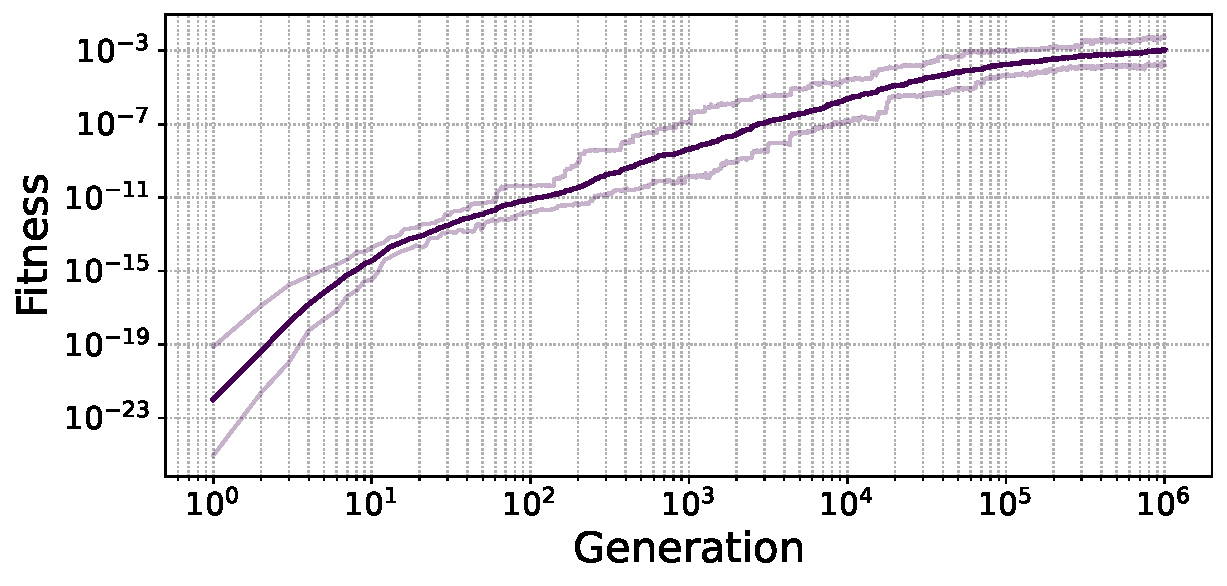
\includegraphics[width=0.75\textwidth]{ploscb/img/all_fitness.pdf}
  \caption[Average fitness during evolution in the advanced model]{Geometric average of the fitness of the best individual in each of the 30 replicates, at every generation.
  Lighter lines represent the first and last decile of the data.}
  \label{fig:ploscb:main_fitness}
\end{figure}

In our simulations, the fitness of the best individual in each population increases over evolutionary time, as shown in Figure~\ref{fig:ploscb:main_fitness}, meaning that evolution is able to select phenotypes that are closer and closer to the target. More precisely, the expression levels of the genes of each type in individuals in our model therefore evolve towards their respective targets, as previously defined in Section~\ref{sec:ploscb:evol_model}.

% Example genome in both environments
\begin{figure}[H]
  \centering
  \begin{elasticrow}[width=\textwidth]
  \elasticfigure{ploscb/img/genome_and_tsc_rep21_env_A.pdf}
  \elasticfigure{ploscb/img/genome_and_tsc_rep21_env_B.pdf}
  \end{elasticrow}
  \caption[Best individual at the end of evolution in one of the replicates in the advanced model, in both environments]{Genome of the best individual at the last generation of replicate 21, evaluated in environments A (left) and B (right).
  In addition to Figure~\ref{fig:ploscb:random_indiv}, the outer ring shows the state of each gene: dark color, activated -- light color, inhibited.
  The inner ring shows the level of transcription-generated DNA supercoiling at every position on the genome: Shades of blue represent negative supercoiling, and shades of red positive supercoiling.}
  \label{fig:ploscb:genomes}
\end{figure}

The genome of an example evolved individual at the end of the simulation is depicted in Figure~\ref{fig:ploscb:genomes}, along with its level of local supercoiling and gene activity in each environment.
Different activation patterns for each gene class are clearly visible on the genome of this individual.
Indeed, all \emph{AB} genes except one are activated (dark blue) in each environment, whereas 19 out of 20 \emph{B} genes are correctly inhibited (light green) in environment A (left) and 18 correctly activated (dark green) in environment B (right).
Conversely, 16 \emph{A} genes are activated (dark red) in environment A, and 16 inhibited (light red) in environment B.

The transcription-generated supercoiling represented in the inner ring furthermore changes consistently with the gene activation patterns between the two environments: red zones, where DNA is positively supercoiled, contain inhibited genes, whereas blue zones, where DNA is negatively supercoiled, contain activated genes.
This individual therefore shows that it is possible for evolution to adjust the gene expression levels of an individual in our model to an environment-dependent target, by relying only on the transcription-supercoiling coupling and on the relative positions of genes on the genome.

% Evolution of gene _activation_ by gene class
\begin{figure}[H]
  \begin{elasticrow}[width=\textwidth]
    \elasticfigure{ploscb/img/gene_activity_env_A_quantile.pdf}
    \elasticfigure{ploscb/img/gene_activity_env_B_quantile.pdf}
  \end{elasticrow}
  \caption[Average number of activated genes during evolution in the advanced model]{Average number of activated genes (with an expression level above $e_{1/2}$) of each type, out of 20, in the best individual at every generation, averaged over the 30 replicates, in environments A (left) and B (right).
  Lighter lines represent the first and last decile of the data.}
  \label{fig:ploscb:gene_activity_by_env}
\end{figure}

\paragraph{Evolution of Class-Specific Gene Expression Levels}
These results are however not specific to this particular individual.
Figure~\ref{fig:ploscb:gene_activity_by_env} shows that, averaging over all replicates, the number of activated genes in each class evolves towards their respective target.
In each environment, the average number of activated \emph{AB} genes quickly reaches nearly 20, its maximum value, as expected from their target; \emph{B} genes follow the same behavior, evolving towards nearly full activation in environment B and nearly full inhibition in environment A.
\emph{A} genes follow a slightly different course, as the number of activated \emph{A} genes seems to converge to approximatively 15 out of the expected 20 in environment A, but continues to decrease towards the expected 0 in environment B by the end of the simulations.

The incomplete match to their target of \emph{A} genes does however not come as a complete surprise.
Environment A is indeed characterized by a positive supercoiling shift $\delta\sigma_A > 0$, while environment B is characterized by a negative supercoiling shift $\delta\sigma_B < 0$.
As positive supercoiling hinders promoter opening, it is more difficult for a gene to have a high transcription rate in environment A than in environment B.
\emph{A} genes must therefore complete the more difficult task of being activated in the ``hard'' environment A, while being inhibited in the ``easy'' environment B.
Differentiated expression levels nonetheless evolve in our model for each type of gene, as a result of the different supercoiling levels imposed by the environmental conditions.

% Final message: evolution of hypercoiling-activated phenotype
\begin{figure}[H]
  \centering
  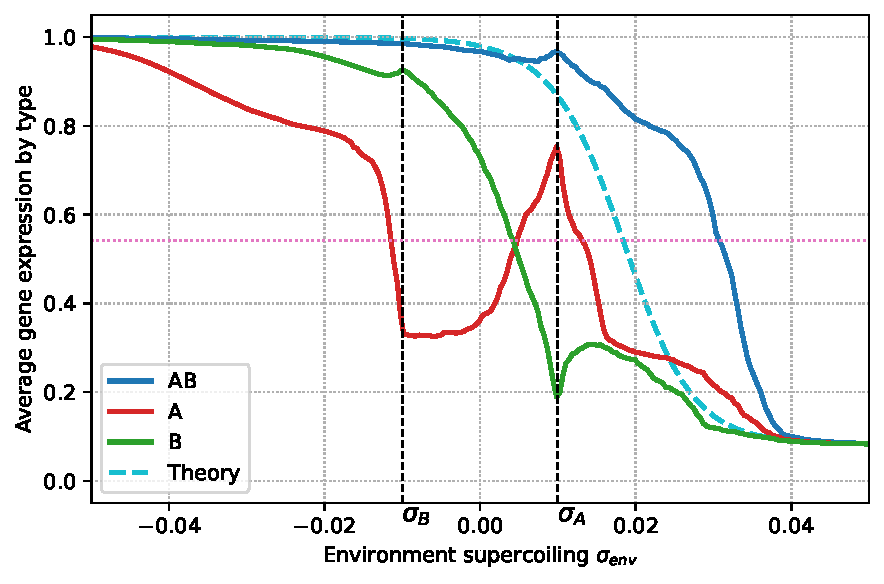
\includegraphics[width=\textwidth]{ploscb/img/activity_sigmas_avg.pdf}
  \caption[Average gene expression as a function of background supercoiling at the end of evolution in the advanced model]{Average gene expression level for each class of gene (\emph{A}, \emph{B}, and \emph{AB}), as a function of the background supercoiling level $\sigma_{basal} + \delta\sigma_{env}$, averaged over the best individual of each of the 30 replicates.
  The dash-dotted light blue line represents the average expression level of genes on a random genome, and the dashed light blue line represents the expression level of a single neighbor-less gene.
  The black vertical lines represent environments A and B, in which individuals evolve during the simulation, and the pink horizontal line marks $e_{1/2}$, the threshold above which a gene is considered active.}
  \label{fig:ploscb:activity_by_sigma}
\end{figure}

\paragraph{Evolution of Relaxation-Activated Genes}
In our model, the expression level of a gene increases exponentially with the opening free energy of its promoter, which itself increases as a sigmoidal function of negative supercoiling.
When measuring the response of an individual's genes to variation in the background supercoiling $\sigma_{basal} + \delta\sigma_{env}$, one could therefore expect a qualitatively similar response.

Figure~\ref{fig:ploscb:activity_by_sigma} shows the responses of genes of different types to the background supercoiling level (as explained in equation~\ref{eq:sigma}), and highlights striking differences between the expression of evolved, random, or isolated genes, as well as between the different gene types in evolved genomes.
The light blue lines in the figure serve as a reference point, showing the response of an isolated, non-interacting gene to environmental supercoiling (dashed line), and the average response (dash-dotted line) of genes on 30 random genomes, generated using the parameters from Table~\ref{tab:param_values}.
While \emph{AB} and \emph{B} genes (blue and green curves) display an expression level that decreases with the level of negative supercoiling, and that remains qualitatively similar to the behavior of random genes (dash-dotted line), \emph{A} genes display a completely different behavior.
These genes show a non-monotonic response to environmental supercoiling, as their expression level decreases until a local minimum in expression at $\delta\sigma_B$, then increases again even though negative supercoiling decreases until a local maximum at $\delta\sigma_A$, before decreasing again like the other kinds of genes.
In other words, \emph{A} genes present a phenotype of activation by environmental relaxation of DNA, for values between $\delta\sigma_B$ and $\delta\sigma_A$, even though the promoter activity of an isolated \emph{A} gene decreases with DNA relaxation.

The transcription-supercoiling coupling therefore provides a regulatory layer that mediates the transcriptional response to the global variation in DNA supercoiling caused by different environments.
Indeed, it remarkably allows in our model for the evolution of a response that is opposite not only to the response displayed by a non-interacting, neighborless gene, but also to the response of genes placed at random on a similar genome, demonstrating the importance of the relative position of genes on the genome.


\subsection{Evolution of Local Genome Organization}

Having characterized the different patterns of gene transcription that evolved in our simulations in response to the two different environmental conditions, we sought to determine the genome organization that necessarily underlies these patterns, since the only difference between individuals in our model is the relative position and orientation of the genes on their genome.

We started by studying genome organization at the local level, and measured the relative abundance of pairs of neighboring genes in every relative orientation: convergent, divergent, or in tandem.
The relative orientation between neighboring genes determines the mode of interaction between these genes, by applying the twin-domain model of transcription-generated supercoiling to the promoter of each gene: mutual activation for divergent genes, mutual inhibition for convergent genes, and activation (resp. inhibition) of the upstream (resp. downstream) gene by the downstream (resp. upstream) gene.

As the different gene types must evolve different activation patterns in each environment to have a high fitness in the model, we separated the pair counts by the type of each gene in the pair, resulting in 9 kinds of pairs.
Finally, in order to quantify the actual strength of the coupling between the genes in a given type of pair, we summed the total level of positive and negative supercoiling generated by the transcription of each gene in the pair at the promoter of the other gene for all relative orientations.
The results are presented in Figure~\ref{fig:ploscb:pair_results}, with the left-hand side panel showing the number of pairs of each kind, and the right-hand side panel the corresponding transcription-generated supercoiling levels.
Several patterns markedly emerge from the data.

\begin{figure}[H]
	\centering
	\begin{elasticrow}[width=\linewidth, sep=1em]
		\elasticfigure{ploscb/img/gene_pair_counts.pdf}
		\elasticfigure{ploscb/img/pos_neg_supercoiling_pairs.pdf}
	\end{elasticrow}
  \caption[Number of gene pairs and supercoiling effect per type of gene pair]{Interactions between pairs of neighboring genes.
  The left-hand side panel shows the number of pairs of each kind, split by the type of the first gene (sub-row) and of the second gene (sub-column) in the pair, and by relative orientation (bars in each sub-panel: convergent, divergent, upstream, or downstream).
  %As there are 20 genes of each type, and each gene appears in two pairs, the total number of pairs in each sub-row and sub-column is always 40.
  For instance, the top-right panel shows the influence of AB genes on B genes, and the bottom-left panel the influence of B genes on AB genes (in the same pairs).
  In that case, there are on average 7.8 \emph{AB} genes directly upstream of a \emph{B} gene (in red), or 7.8 \emph{B} genes directly downstream of an \emph{AB} gene (in green) on an evolved genome.
  % Talk about induced supercoiling?
  The right-hand side panel shows, for each kind of pair, the total amount of positive (red) and negative (green) transcription-generated supercoiling due to each gene type (sub-row) measured at the promoter of each gene type (sub-column), summing over all orientations, but in each environment.
  All data is averaged over the best individual of each of the 30 replicates, and box plots indicate the median and dispersion between the replicates.}
  \label{fig:ploscb:pair_results}
\end{figure}

% Divergent pairs: AB
\paragraph{Genomes Are Enriched in Divergent \emph{AB}/\emph{AB} Gene Pairs}
The most frequently found kind of gene pair in the evolved genomes is divergently oriented \emph{AB}/\emph{AB} pairs.
13 such pairs are found on average (see the \emph{AB}/\emph{AB} sub-panel on the left-hand side of Figure~\ref{fig:ploscb:pair_results}), out of a possible maximum of 20 (since any given gene can only be part of a single divergent pair), meaning that two-thirds of \emph{AB} genes are part of a divergent pair with another \emph{AB} gene.
The mostly divergent \emph{AB}\emph{AB} gene pairs generate an average negative supercoiling of around -0.012 at their promoters, in both environments (summing the positive and negative bars in the \emph{AB}/\emph{AB} sub-panel on the right-hand side of Figure~\ref{fig:ploscb:pair_results}).
This value is comparable in magnitude to but has the opposite sign than the shift in supercoiling caused by environment A ($\delta\sigma_A = 0.01$), showing that the interaction between neighboring genes can locally counteract the global shift in supercoiling caused by this environment in order to maintain high gene expression levels.

% Divergent pairs: A/A and B/B too, but not A/B
Genomes also contain divergent \emph{A}/\emph{A} and \emph{B}/\emph{B} gene pairs, although less frequently than divergent \emph{AB}/\emph{AB} pairs.
As both \emph{A} genes and \emph{B} genes must be conditionally expressed or inhibited depending on the environment, the unconditionally positive feedback loop resulting from a divergent orientation seems less evolutionarily favorable for \emph{A}/\emph{A} or \emph{B}/\emph{B} pairs than for \emph{AB}/\emph{AB} pairs.
Divergent \emph{A}/\emph{A} and \emph{B}/\emph{B} pairs moreover result in slightly weaker interactions (middle and bottom-right sub-panel of the right-hand side of Figure~\ref{fig:ploscb:pair_results}), in the environment in which these genes are active.
On the contrary, divergent \emph{A}/\emph{B} gene pairs are almost never found, and this is consistent with theoretical expectation, since \emph{A} and \emph{B} genes must no be expressed in the same environment.

The local organization of the genome in divergent \emph{AB}/\emph{AB} gene pairs therefore seems to be favored by evolution, as this pattern allows for a high expression of these genes in both environments, while divergent \emph{A}/\emph{B} gene pairs, which would lead to a lower fitness, are oppositely very rarely found in evolved genomes.

% Convergent pairs: A and B, mostly
\paragraph{Genomes are Enriched in Convergent \emph{A}/\emph{B} Gene Pairs}
The pattern in which \emph{B} genes appear most frequently, and \emph{A} genes very frequently (just after divergent \emph{A}/\emph{A} pairs), is in convergent \emph{A}/\emph{B} gene pairs.
In this case, each gene in the pair should theoretically inhibit the expression of the other gene.
In environment A, \emph{A} genes indeed generate an average positive supercoiling variation of 0.01 at the promoter of convergently oriented \emph{B} genes (the effect of \emph{B} genes on convergent \emph{A} genes in environment B is similar), decreasing their expression with a strength that is again comparable to the environmental change in supercoiling, whiles B genes are mostly inhibited and therefore do not impact \emph{A} genes.
In environment B, it is instead \emph{B} genes that strongly inhibit \emph{A} genes through the generation of positive supercoiling.

Convergently oriented \emph{A}/\emph{B} gene pairs therefore form toggle switches, or bistable gene regulatory circuits, in which the expression of one gene represses the expression of the other gene~\citep{gardner2000}.
In accordance with the targeted expression patterns of \emph{A} and \emph{B} genes, we therefore observe that the local organization of the genome into toggle switches, like the divergent \emph{A}/\emph{B} pairs, is favored by evolution in order to produce environment-dependent differentiated expression levels.


\subsection{Local Interactions Do Not Recapitulate the Regulatory Network}

In order to understand the extent to which the gene regulatory network generated by the transcription-supercoiling coupling can be reduced to the local organization into pairs of genes described above, we expanded our scope to study the behavior of subnetworks of neighboring genes of increasing sizes.

\begin{figure}[H]
  \centering
  %\begin{subfigure}[t]{\textwidth}
    %\centering
    %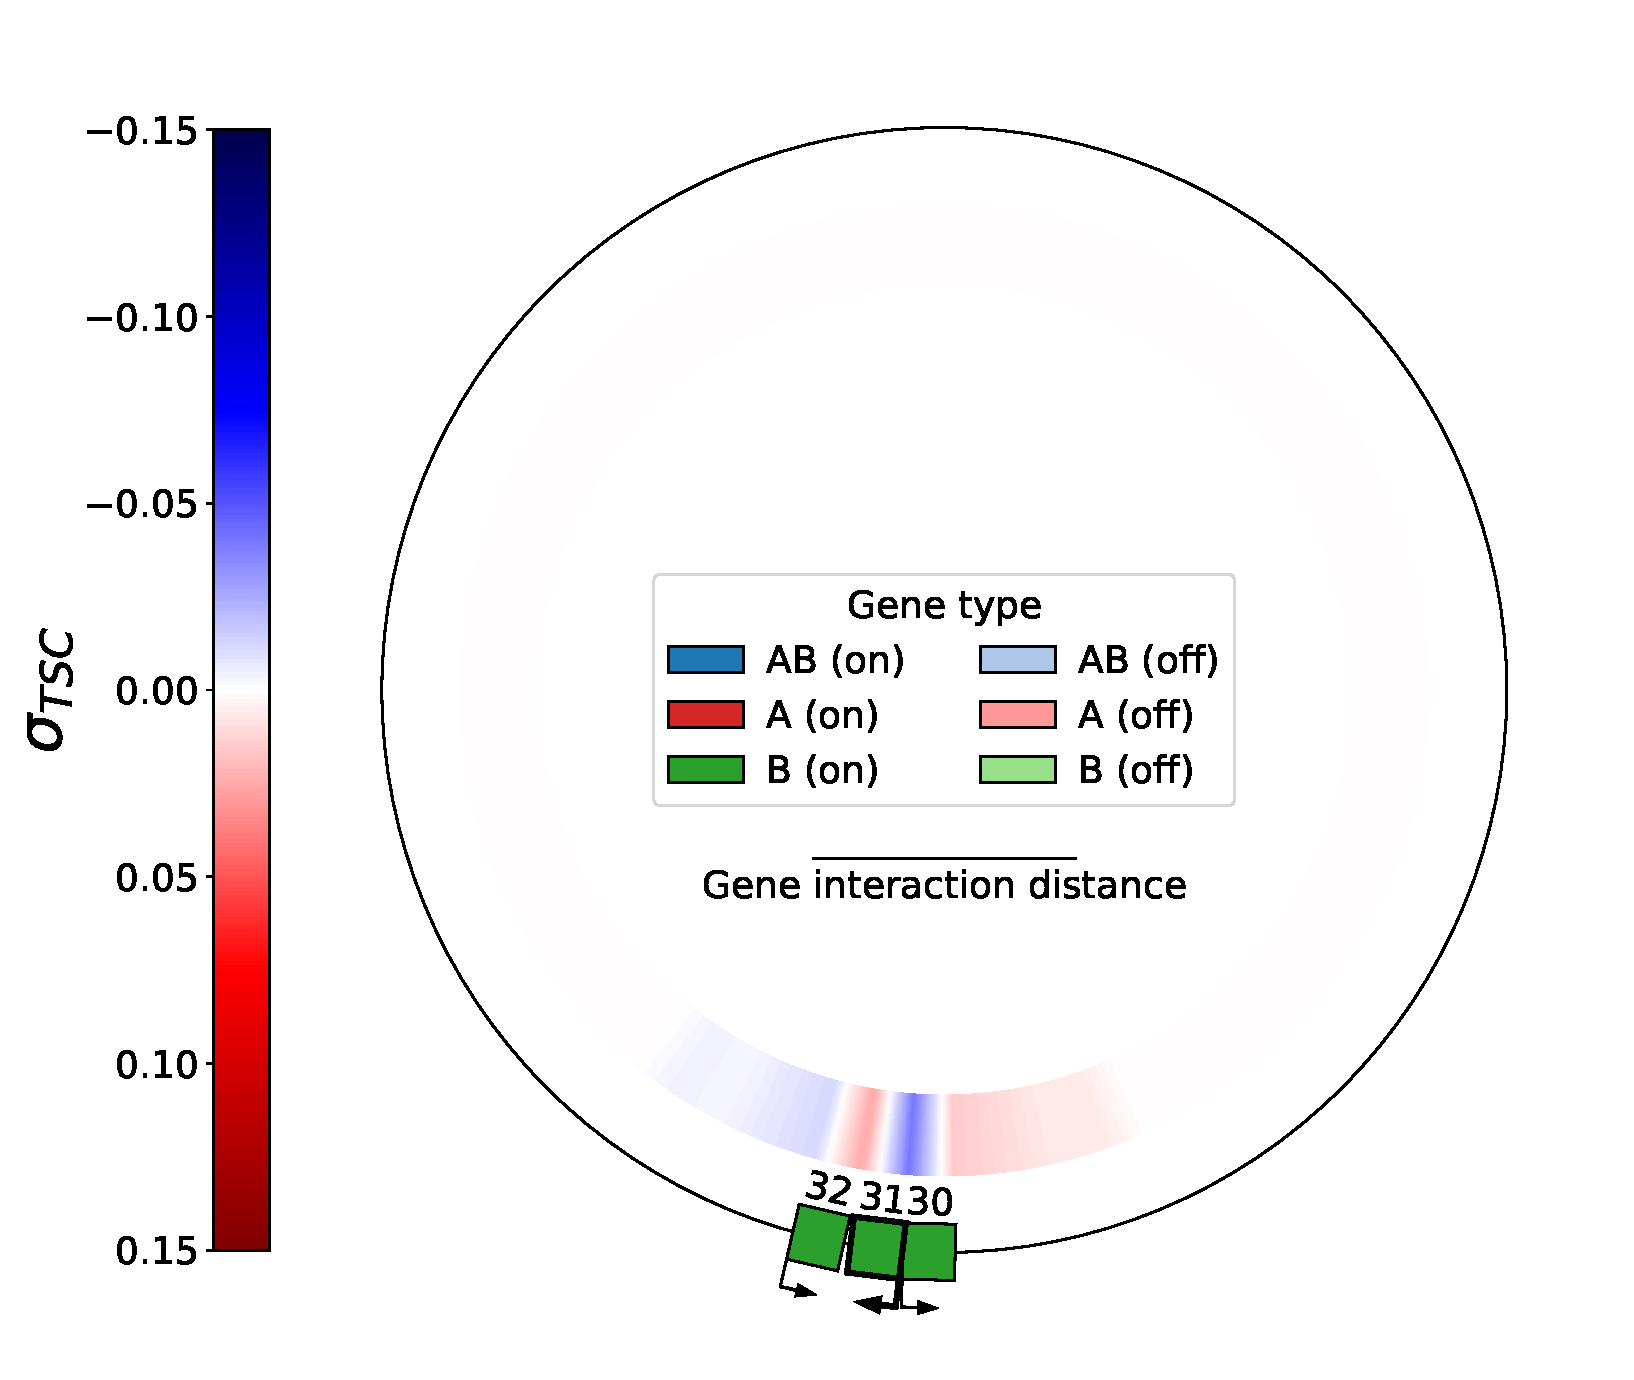
\includegraphics[height=7cm]{ploscb/img/sub_3_genes_30_env_A.pdf}
    %\hspace{-0.5cm}
    %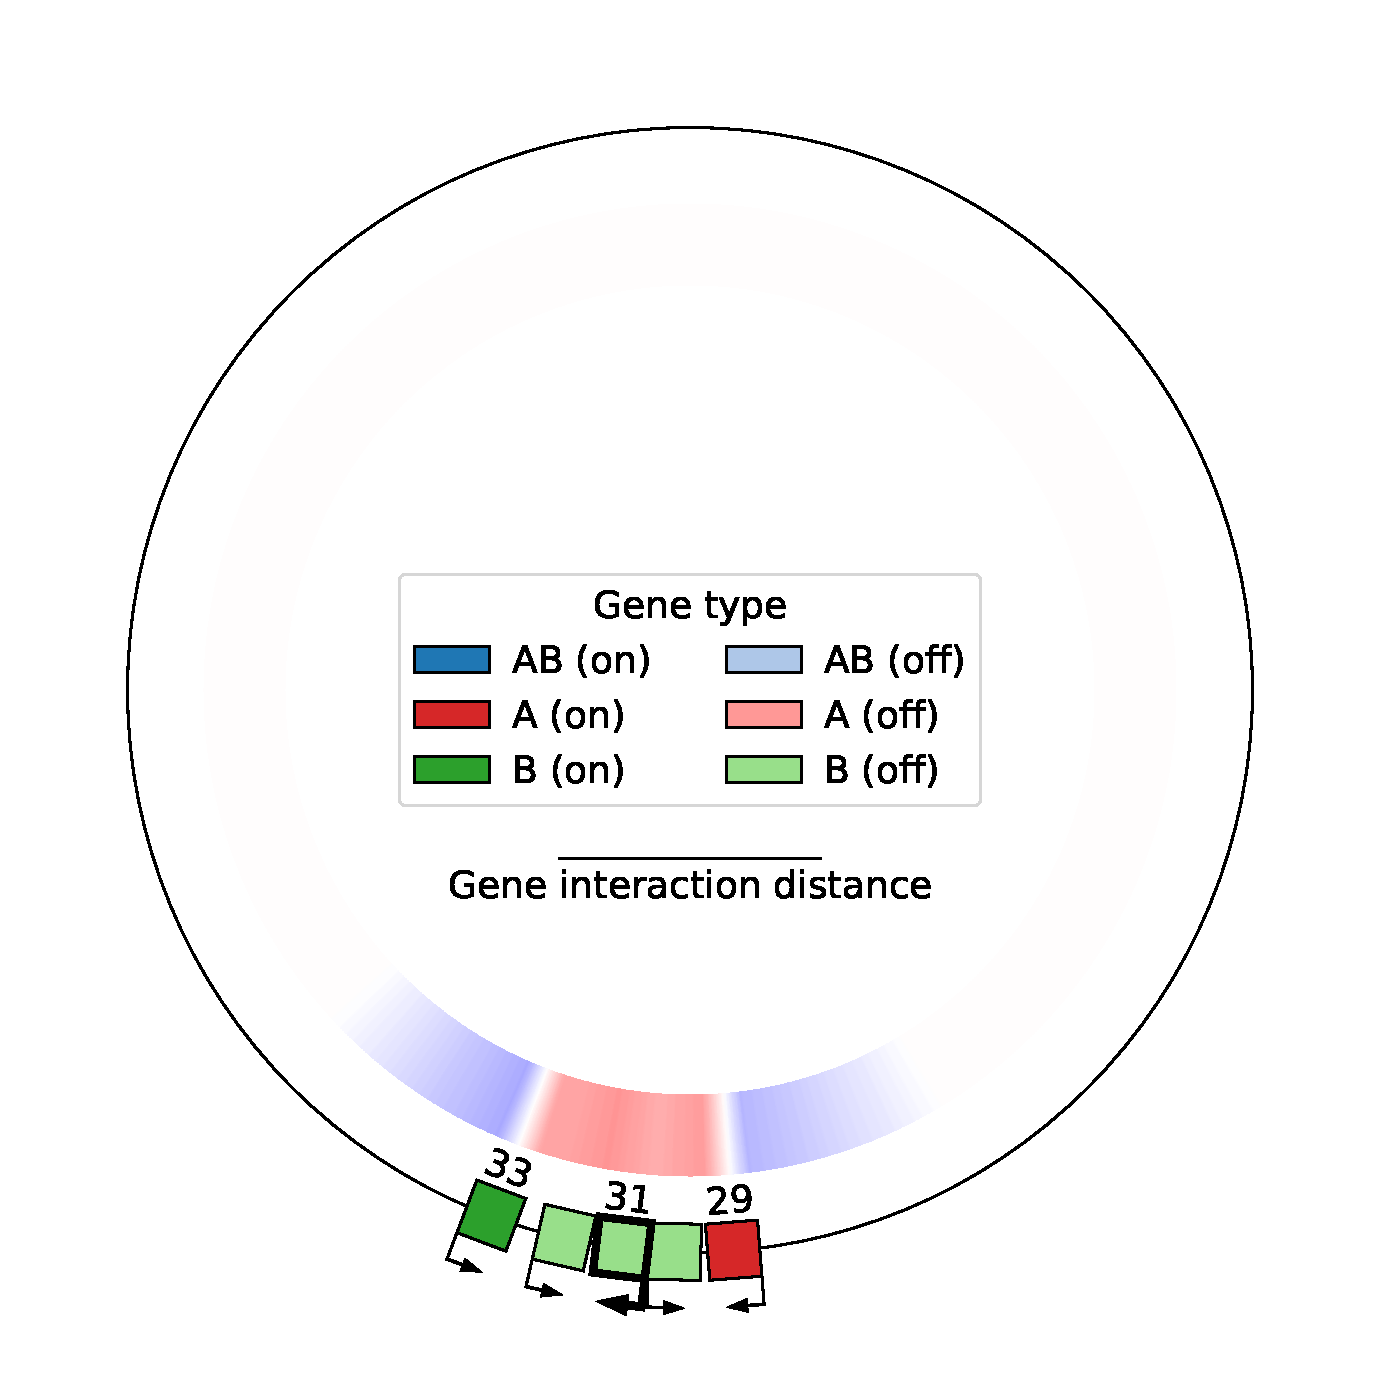
\includegraphics[height=7cm]{ploscb/img/sub_5_genes_29_env_A.pdf}
  %\end{subfigure}
  \begin{elasticrow}[width=\linewidth]
		\elasticfigure{ploscb/img/sub_3_genes_30_env_A.pdf}
		\elasticfigure{ploscb/img/sub_5_genes_29_env_A.pdf}
	\end{elasticrow}
  \begin{elasticrow}[width=\linewidth]
		\elasticfigure{ploscb/img/sub_7_genes_03_env_B.pdf}
		\elasticfigure{ploscb/img/sub_9_genes_02_env_B.pdf}
	\end{elasticrow}
  \caption[Example minimal subnetworks needed for gene inhibition in an evolved individual]{Top: subnetworks of size 3 (left) and 5 (right) centered around gene 31 (of type \emph{B}, in bold) of the best individual at the end of replicate 21, evaluated in environment A.
  Bottom: subnetworks of size 7 (left) and 9 (right), centered around gene 6 (of type \emph{A}, in bold) of the same individual, evaluated in environment B.
  }
  \label{fig:ploscb:subnetwork_examples}
\end{figure}

For every odd subnetwork size $k$ between 1 and the genome size, and for every gene on the genome, we extracted the subnetwork of size $k$ centered around that gene, and computed the expression level of every gene in the subnetwork, in the same way as for a complete genome, in each environment.
This allowed us to compute the minimum subnetwork size at which a gene has the same activation state as in the complete genome, which we interpret as an indicator of the complexity of the interaction network necessary to produce the activation state of that gene in the complete genome.
Two representative examples are presented in Figure~\ref{fig:ploscb:subnetwork_examples}, and the complete results are then shown in Figure~\ref{fig:ploscb:min_subnetwork}.

Figure~\ref{fig:ploscb:subnetwork_examples} depicts the subnetworks that are needed in order to obtain the inhibition of a representative gene of type \emph{A} in environment B, and of a representative gene of type \emph{B} in environment A, taken from the genome of an evolved individual.
The \emph{B} gene is not inhibited by a subnetwork of size 3, but needs a subnetwork of size 5 to be inhibited, and similarly, the \emph{A} gene is not inhibited by a subnetwork of size 7, but needs a subnetwork of size 9 to be inhibited.
In each case, increasing the size of the subnetwork by two (one gene on each side) completely changes the resulting gene expression levels, alongside with the associated level of transcription-generated supercoiling.
Indeed, in the top example, all 3 genes in the small subnetwork switch states when evaluated inside the larger subnetwork, and in the bottom example, the two \emph{B} genes and two out of the three central \emph{A} genes switch activation states when moving from the small to the large subnetwork.
In these examples, the activity of a gene is therefore not only dependent on its closest neighbors, but on a quite larger section of the genome.

\begin{figure}[H]
  \centering
  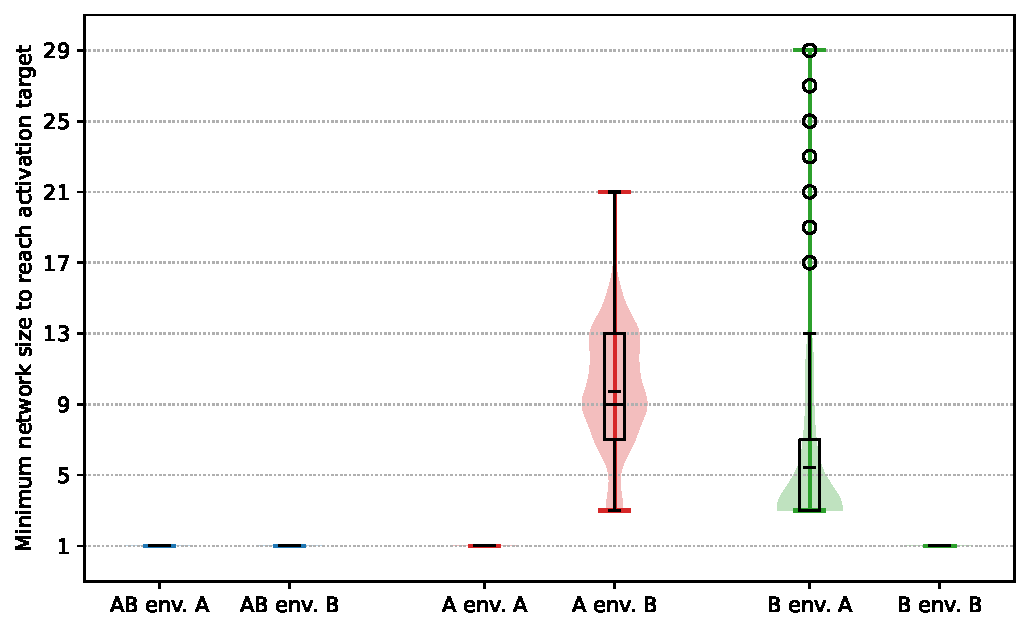
\includegraphics[width=\textwidth]{ploscb/img/min_network_size.pdf}
  \caption[Minimal subnetwork size needed to obtain the correct activation state per gene type]{Minimal contiguous subnetwork size needed for the central gene in the subnetwork to have the same activation state as in the complete genome, for each gene type, and in each environment, for every gene of the best individual at the end of each replicate.
  In each case, a box plot showing quartiles and fliers is overlaid on a violin plot representing the whole distribution, and the mean is represented by a smaller tick.
  The data is computed only for genes which present the correct activation state in both environments, which represents 97,7\% of \emph{AB} genes, 92,7\% of \emph{B} genes and 53,2 \% of \emph{A} genes.}
  \label{fig:ploscb:min_subnetwork}
\end{figure}

We averaged this data over every gene that presents the correct activation state in each environment, in the best individual of every replicate, and very different patterns once more appear, depending on whether the targeted behavior for the gene is activation or inhibition, as depicted in Figure~\ref{fig:ploscb:min_subnetwork}.
For \emph{AB} genes in both environments, as well as for \emph{A} genes in environment A and \emph{B} genes in environment B, the experimentally obtained minimum subnetwork size is 1, which is consistent with the expression profile of an isolated gene, shown in Figure~\ref{fig:ploscb:activity_by_sigma}: With a basal supercoiling value of $\sigma_{basal} = -0.06$, an isolated gene already experiences a high expression level in both environments, even without interactions.

When the evolutionary target of the gene is inhibition, that is for \emph{A} genes in environment B and for \emph{B} genes in environment A, the picture is however quite different.
In this case, a significantly larger subnetwork is needed in order to obtain inhibition of the central gene: The median subnetwork size is 9 (4 genes on each side) for \emph{A} genes.
For \emph{B} genes, the median size is smaller than for \emph{A} genes, but higher than when the target is activation: Genes always need at least a subnetwork of size 3 (1 gene on each side), and several outliers need a subnetwork of more than 20 genes.

The gene regulatory networks evolved through the transcription-supercoiling coupling therefore exhibit a structure that cannot always be summarized by the pairwise interactions between neighboring genes, but that can on the contrary require the participation of a significantly larger number of genes in order to make genes display the same activation state as in the full genome.


\subsection{A Whole-Genome Gene Regulatory Network}

The effect of the transcription of every gene on the local supercoiling at every other gene (which decreases linearly with distance) provides a natural graph to represent the interactions between the genes in the genome of an individual.
However, as the effective impact of a gene on the expression of other genes depends on the transcription level of that gene, this theoretical graph provides an inaccurate picture of the gene interactions that actually take place, as every gene ends up expressed at a different level.
In order to characterize more finely the gene regulatory networks that evolve in our experiments, we therefore constructed a different graph, which we call the effective interaction graph, using transcriptional gene knockouts.

\begin{figure}[H]
  \centering
  \begin{elasticrow}[width=\linewidth]
		\elasticfigure{ploscb/img/ko_genome_and_tsc_env_A_gene_36.pdf}
		\elasticfigure{ploscb/img/ko_genome_and_tsc_env_B_gene_36.pdf}
	\end{elasticrow}
  \caption[Example evolved individual with a knocked-out gene, evaluated in both environments]{Knockout of gene 36 (of type \emph{AB}, in bold, colored white) of the best individual at the end of replicate 21, evaluated in environments A (left) and B (right).
  Hatched genes represent genes whose activation state was switched by the knockout compared to their state in the original genome.
  The inner ring represents the absolute difference in the level of local supercoiling $|\Delta\sigma_{TSC}|$ between the knockout genome and the original genome (in Figure~\ref{fig:ploscb:genomes}).}
  \label{fig:ploscb:ko_genomes}
\end{figure}

\paragraph{Transcriptional Gene Knockouts}
A transcriptional gene knockout (or simply gene knockout in the manuscript) completely suppresses the transcription of a gene, adapting the principle of gene knockouts to the transcription rather than the translation step of gene expression.
In order to knock out a gene in an individual in our model, we simply set the transcription rate of that gene to zero during every step of the computation of the gene expression levels of that individual.
This virtually removes the knocked-out gene from the genome, while keeping the intergenic distance between its upstream and downstream neighbors unchanged, and mimics a loss of function its the promoter.
The result of such a knockout on the genome of an evolved individual is shown in Figure~\ref{fig:ploscb:ko_genomes}.
The knocked-out gene is gene 36, which is of type \emph{AB} and originally activated in both environments (see Figure~\ref{fig:ploscb:genomes} for the original genome).
We can see that, in environment A, knocking out this gene results in a switch of the activation state for 7 genes (hatched in the left-hand side of Figure~\ref{fig:ploscb:ko_genomes}), that are not all contiguously located, and in local supercoiling changes that propagate to the bottom left third of the genome, to a distance that is larger than the gene interaction distance.
In environment B, knocking out this gene results in milder supercoiling changes that do not lead to the switch of any gene.
In this example, knocking out even a single gene can therefore substantially affect gene expression levels, significantly switching the activation state of other genes on the genome, even when they are out of reach of direct interaction with the knocked-out gene.

\begin{figure}[H]
  \centering
  \hspace{-1cm}
  \begin{subfigure}[c]{0.73\textwidth}
    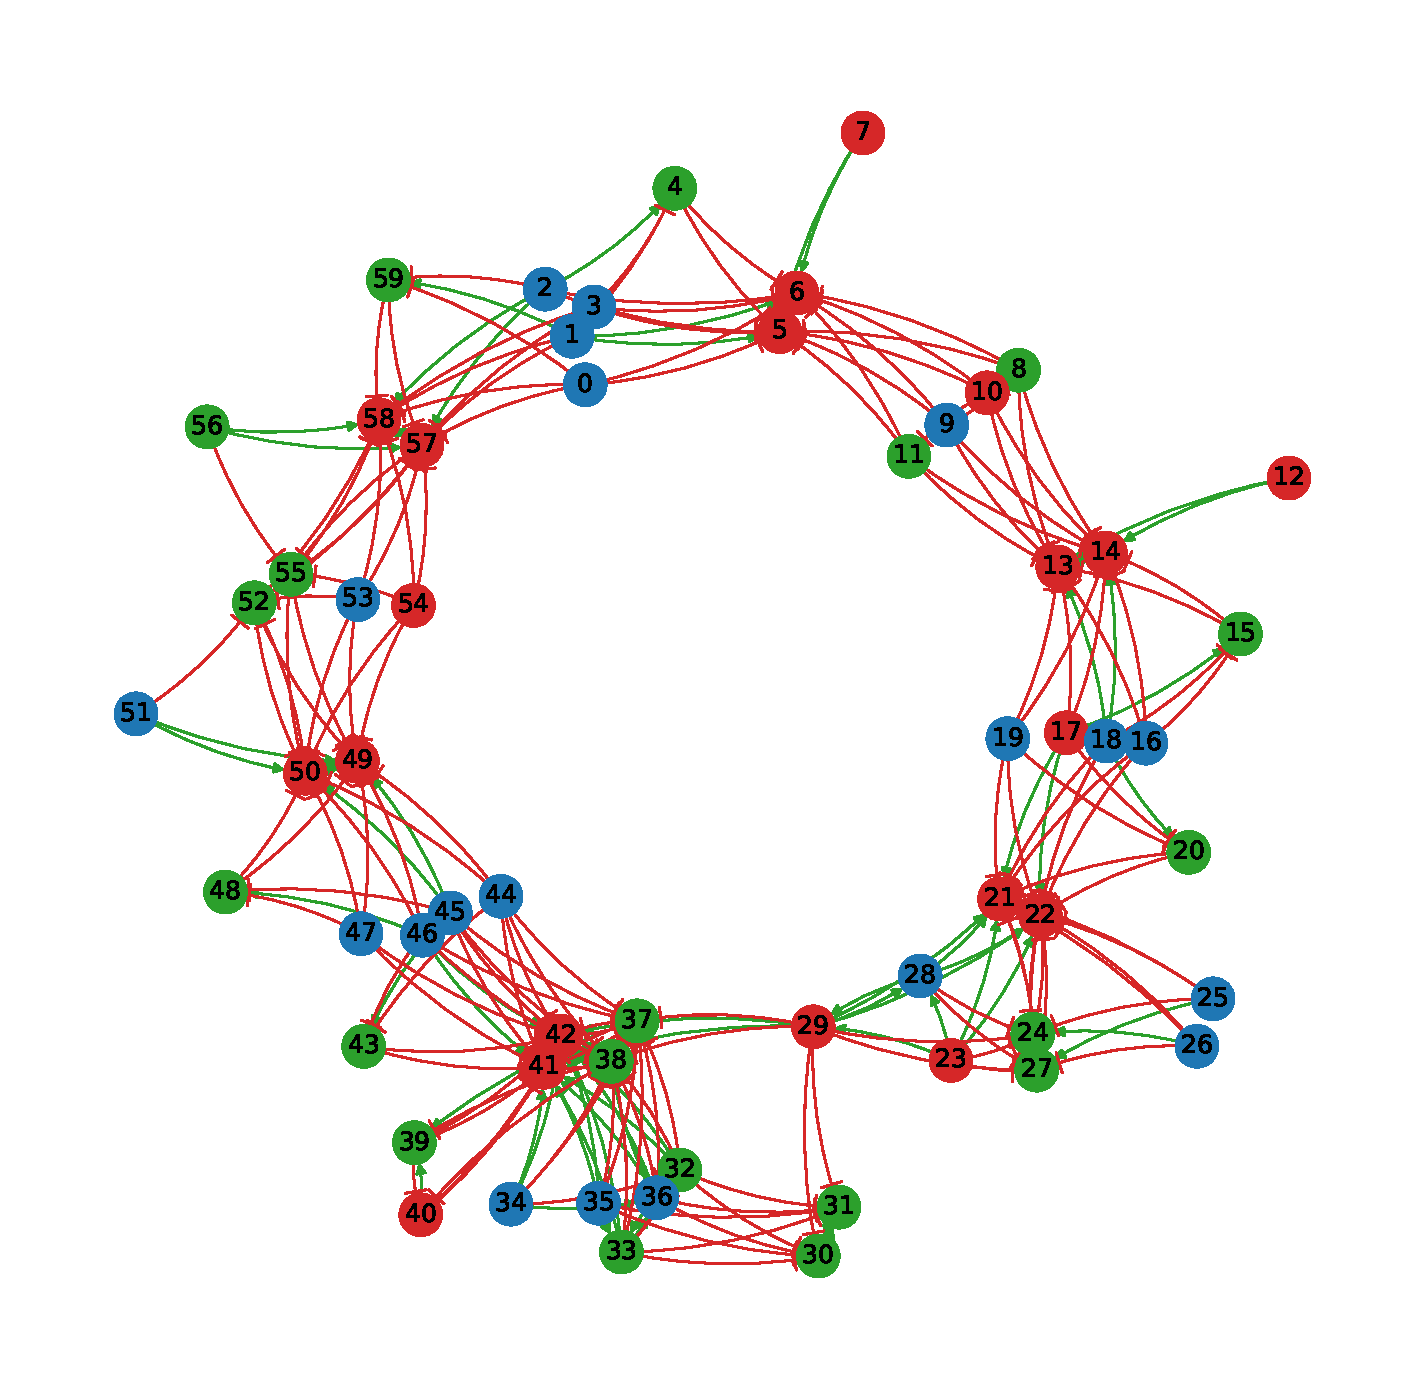
\includegraphics[width=\textwidth]{ploscb/img/combined_effective_graph_rep21_graphviz.pdf}
  \end{subfigure}
  \hspace*{-0.75cm}
  \begin{subfigure}[c]{0.29\textwidth}
    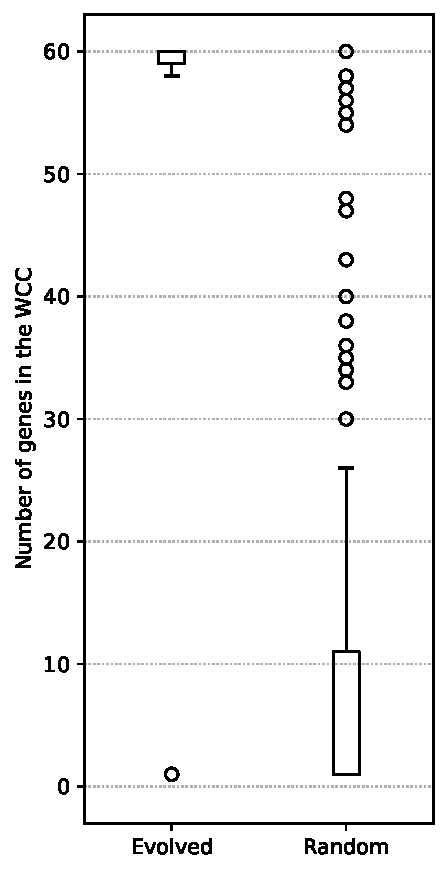
\includegraphics[width=\textwidth]{ploscb/img/effective_graph_wcc_distr.pdf}
  \end{subfigure}
  \caption[Effective interaction graph of an evolved individual, and distribution of effective interaction graph WCCs in evolved and random individuals]{Left: effective interaction graph of the best individual at the last generation of replicate 21, obtained by knocking out each gene and measuring the resulting gene switches in each environment.
  Activation edges are drawn in green, and inhibition edges in red.
  The numbering of the genes is the same as in Figures~\ref{fig:ploscb:genomes},~\ref{fig:ploscb:ko_genomes} and~\ref{fig:ploscb:ko_genomes}.
  Right: distribution of weakly connected component (WCC) sizes in the effective interaction graphs of the evolved individuals (left) and the random individuals (right).}
  \label{fig:ploscb:ko_graph}
\end{figure}

\paragraph{Constructing Effective Interaction Graphs}
In order to construct the effective interaction graph introduced above, we simply add an edge from a gene to every other gene whose activation state is switched by knocking out that gene, in one environment or the other.
If the knockout switches off a gene that was activated in the complete genome, we mark the edge as an activation edge, meaning that the knocked-out gene was necessary to activate the switched gene.
If the knockout switches on a gene that was inhibited in the complete genome, we conversely mark the edge as an inhibition edge.
If knocking out a gene switches the same gene in the two environments, we only add the edge once (we do not build a multigraph).
The effective interaction graph of our example individual is presented on the left-hand side of Figure~\ref{fig:ploscb:ko_graph}.
In the case of this individual, there is a single weakly connected component (WCC), meaning that all genes interact as part of a single whole-genome regulatory network; this is the case in the best individual of 26 out of the 30 replicates.

\paragraph{Structure of the Effective Interaction Graphs}
We computed the effective interaction graph of the best individual in each replicate, and compared these graphs with the effective interaction graphs of 30 random individuals drawn using the same genome parameters (in Table~\ref{tab:param_values}).
The results are presented on the right-hand side of Figure~\ref{fig:ploscb:ko_graph}.
The effective interaction graphs of evolved individuals are clearly different from the interaction graphs of random individuals.
We can see that the evolved genomes have WCC sizes of 58 to 60 genes, comprising nearly every to every gene on the genome, along with very few single-gene WCCs (left).
On the other hand, WCC sizes in the random genomes span the whole range from single-gene to whole-genome WCCs, with most of the connected components counting less than 10 genes (right).

\begin{figure}[H]
  \begin{subfigure}[t]{0.49\textwidth}
    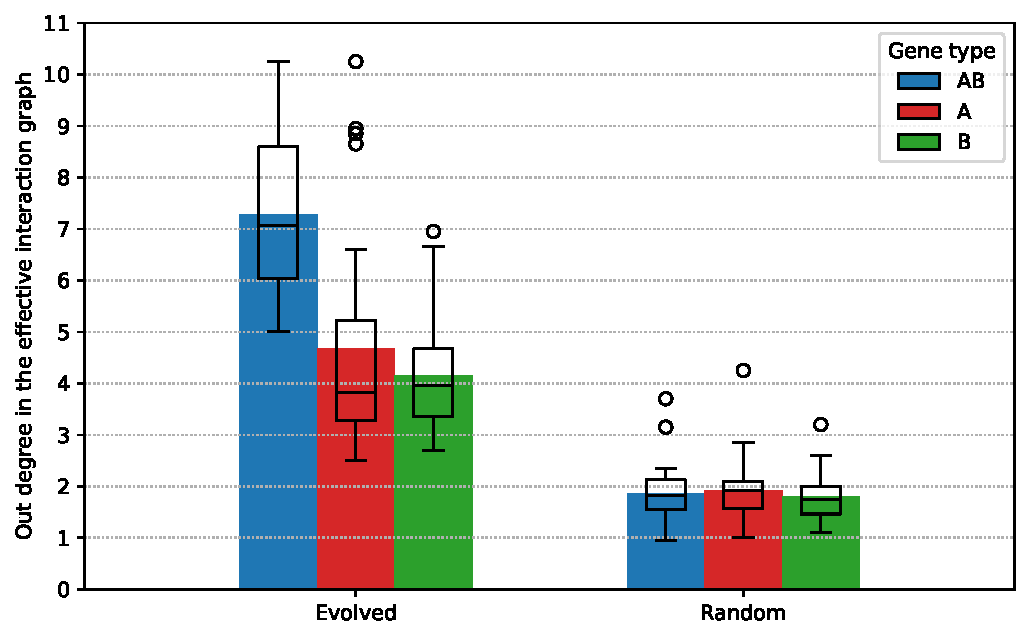
\includegraphics[width=\textwidth]{ploscb/img/effective_graph_combined_out_degree.pdf}
  \end{subfigure}
  \begin{subfigure}[t]{0.49\textwidth}
    \includegraphics[width=\textwidth]{ploscb/img/effective_graph_combined_in_degree.pdf}
  \end{subfigure}
  \caption[Average in- and out-degree of effective interaction graph nodes for evolved and random individuals]{Left: average out-degree (number of genes switched by knocking out a given gene) of the nodes in the effective interaction graph, separated by gene type, for evolved and random individuals.
  Right: average in-degree (number of genes whose knockout switches a given gene) of the nodes in the effective interaction graph, separated by gene type, for evolved and random individuals.}
  \label{fig:ploscb:ko_data}
\end{figure}

The evolved genomes are indeed much more connected than the random genomes, as we can see in Figure~\ref{fig:ploscb:ko_data}, which presents the out- and in-degree of genes (averaged by gene type) in the effective interaction graphs of the genomes.
The left-hand side of Figure~\ref{fig:ploscb:ko_data} shows the average out-degree of each gene type, or the number of genes that are switched by knocking out a gene of that type.
While knocking out a gene in a random genome switches the state of just under 2 other genes on average, the figure is much higher in the evolved genomes.
Knocking out \emph{A} and \emph{B} genes switches 4 other genes on average, and knocking out \emph{AB} genes up to 7 other genes;
\emph{AB} genes therefore play a quantitatively more important regulatory role than \emph{A} genes or \emph{B} genes, which can be explained by the fact that \emph{AB} genes are activated in both environments, while most \emph{A} and \emph{B} genes are inhibited in one environment or the other.

When looking at the in-degree of the genes, or the number of genes whose knockout will make a given gene switch activation states, we can see that the evolved genomes are again much more connected than the random genomes, and that the in-degree depends on the type of the gene.
Indeed, \emph{AB} genes are only switched by one other gene on average, meaning that their activation state is robust to perturbations in the regulatory network.
The robustness of \emph{AB} gene state is expected, as these genes must have the same activation state in both environments.
On the contrary, \emph{A} genes and \emph{B} genes have an in-degree that is much higher, meaning that their activation state relies on the regulatory action of a large number of other genes, making them more sensitive to the variations between the two environments.

The evolution of the the relative positions of genes on the genome, by leveraging the feedback loop between the transcription of neighboring genes that is mediated by DNA supercoiling, therefore results in our model in the emergence of gene regulatory networks that connect the whole genome into a single entity, rather than a juxtaposition of independent subnetworks.
The network structure that evolves furthermore allows genes to dampen, or amplify, the result of the environmental shift in supercoiling on their activation states, as required by their evolutionary targets.

\section{Discussion and Perspectives}

DNA supercoiling, through its effect on promoter activation~\citep{forquet2021}, is an important actor of the regulatory response of bacteria to changing environmental conditions~\citep{martisb.2019}.
But supercoiling itself is in return impacted by transcription, as presented in the twin-domain model of~\cite{liu1987}.
Indeed, transcription has been shown to play a major role in shaping the bacterial DNA supercoiling landscape~\citep{visser2022}.
Taken together, these observations raise the question of the extent to which the position itself of genes on the genome can regulate their activity, via the coupling of the transcription levels of neighboring genes through local changes in DNA supercoiling.

In order to assess the theoretical possibility of the evolution of such a gene regulatory network, and to determine the potential consequences of the evolution of such a network on the organization of the genome, we developed in this work an evolutionary model of the transcription-supercoiling coupling (expanding upon a proof-of-concept presented in~\cite{grohens2021}), in which populations of individuals must evolve differentiated gene expression levels in response to different environmental conditions, with the transcription-supercoiling coupling as the only regulatory mechanism and inversions as the only mutational operator.
As a the dynamic supercoiling level between actively transcribed genes would be very difficult to model quantitatively, our model voluntarily stays very simple in this regard, and focuses instead on providing a qualitative overview of the range and complexity of the regulatory interactions between neighboring genes that can be mediated by the transcription-supercoiling coupling.

We showed that, in this model, gene regulation by DNA supercoiling is indeed a sufficient mechanism to evolve environment- and gene-specific patterns of activation and inhibition.
In particular, we observed the emergence of genes that are more expressed in a relaxation-inducing environment (or relaxation-activated genes), even though this behavior goes against the facilitated opening of the -10 promoter element by RNA polymerase during the initiation of transcription~\citep{forquet2021}.
%, and is accordingly quite unfrequent in \emph{in vitro} transcription data (where isolated promoters are expressed on plasmids).
This property has been analyzed in detail \emph{in vivo} in the classical example of the \emph{gyrA} promoter, and was shown to result from the unusual sequence of that promoter~\citep{menzel1987}, but for many other genes, this property is less firmly established and depends on the experimental conditions, with experiments finding a proportion of relaxation-activated genes varying between 27\% and 70\% in \emph{S. enterica}~\citep{pineau2022a}.
Our results demonstrate that this behavior can result not only from the specific sequence of the promoter (as for the \emph{gyrA} promoter), but also from the local genomic organization (as suggested in~\cite{elhoudaigui2019}), and confirm the importance of this additional mode of regulation for the first time in an evolutionary simulation.
%A global relaxation of DNA can indeed result in the local hypercoiling, and hence high expression, of genes that happen to be located in the right genetic context.
%The regulation of gene expression by local changes in DNA supercoiling therefore provides a possible causal mechanism for the activity of the relaxation-activated genes found in \emph{E. coli}~\citep{peter2004,sobetzko2016}, \emph{S. enterica}~\citep{webber2013}, or \emph{D. dadantii}~\citep{pineau2022}.

We found that evolved genomes in the model are enriched in divergent pairs of always-active genes, as well as in convergent pairs that act as bistable toggle switches~\citep{gardner2000,johnstone2022}; the evolution of such systems substantiates the theoretical predictions made by models that explicitly describe the movement of RNA polymerases during gene transcription, such as~\cite{sevier2021}.
Then, we showed that the local organization of the genome into convergent or divergent pairs of genes is not sufficient to explain the transcriptional response of individuals to different environments, but that larger subnetworks can be required to selectively inhibit genes in specific environments.
Such regulation of gene expression through interaction with groups of neighboring genes could help explain the evolutionary persistence of synteny groups between \emph{E. coli} and \emph{S. enterica}~\citep{junier2016}, as well as through the evolutionary history of \emph{B. aphidicola}~\citep{brinza2013}.
Indeed, we show that local interactions can play a role in regulating the expression of neighboring genes, and genomic rearrangements might disrupt these local interactions.
Finally, we used transcriptional knockouts, adapting the  classical tool of gene knockouts~\citep{baba2006} to our transcription-centric model, in order to characterize the evolved gene regulatory networks in further detail.
We first showed that these regulatory networks integrate the entire genome of evolved individuals into a single connected unit, in opposition to the sparser, disconnected regulatory networks displayed by randomly generated individuals.
Then, we showed that the structure of these networks leverages the transcription-supercoiling coupling to increase or decrease the sensitivity of genes to perturbations in the regulatory network, strengthening the differentiated expression patterns that are the evolutionary target for each gene type.

All in all, our simulations demonstrate that the transcription-supercoiling coupling provides a regulatory mechanism that is precise enough for the evolution of complex regulation patterns that only depend on the arrangement of genes on the genome.

Several work directions still remain open to investigation.
From an evolutionary perspective, the experimental framework in which we tested our model is at present very simple, and could be extended.
The desired gene expression levels in our model are binary, targeting maximal or minimal transcription, but could be replaced by an arbitrary level between these values for each gene, in order to see whether the local organization into pairs as well as the whole-genome regulatory network that we described are preserved under these less constrained conditions.
Similarly, we could refine the environmental challenge faced by individuals by evaluating them in each environment in succession, rather than separately, or by continuously changing the environment over evolutionary time.
From a theoretical perspective, a range of mechanistic biophysical models of the transcription-supercoiling coupling have been put forward, with different hypotheses underpinning the coupling:~\cite{brackley2016} shows a phase transition in the transcription regime as the number of transcribing RNA polymerases increases;~\cite{sevier2021} shows that bursty transcription can emerge from the transcription-supercoiling coupling; and~\cite{meyer2014} and~\cite{elhoudaigui2019} try to predict gene expression levels quantitatively from the local DNA supercoiling level.
An important vindication of these theoretical approaches to the interplay between supercoiling and transcription would therefore be to verify the extent to which these models, including ours, conform to one another as the level of abstraction changes.
Moreover, integrating a model of gene regulation by DNA supercoiling into a more comprehensive evolutionary model of the genome that allows for classical gene regulation via transcription factors, such as the model presented in~\cite{crombach2008}, would help shed light on the coevolution between the different modes of gene regulation that are available to bacterial genomes.
Finally, from an experimental perspective, a better understanding of the regulatory interactions caused by the transcription-supercoiling coupling could help design more reliable synthetic genetic constructs, as explored in~\cite{johnstone2022}.


\section{Conclusion}

To the best of our knowledge, our work is the first to model the regulatory role of supercoiling on transcription at a many-gene scale, using evolutionary simulations.
It demonstrates the importance of the direct interactions between genes that are mediated by local changes in DNA supercoiling on their transcription rates, as well as the precision and versatility of the regulatory activity stemming from these interactions.
For experimentalists, it provides an underlying theory that could help explain the heterogeneous transcriptomic response (with both up- and down-regulation of multiple genes) observed in bacteria confronted to supercoiling variations, due among others to virulence-inducing environments~\citep{dorman2019} or to gyrase-inhibiting antibiotics~\citep{delacampa2017}.
For evolutionists, it provides a plausible evolutionary rationale for the observed conservation of local gene order between closely related bacteria~\citep{junier2016} and along evolutionary histories~\citep{brinza2013}.
Finally, for synthetic biologists, it provides a theory to help predict in finer detail the gene transcription levels that can be expected from a given gene syntax~\citep{johnstone2022}, which could help design more robust genetic circuits.


\appendix

\chapter{Covid-19 Task Force}
\label{chap:covid}

At the start of the Covid-19 pandemic (March-April 2020), I took part in an Inria task force that was created to provide scientific expertise to external stakeholders.
In particular, we worked with the Assistance Publique-Hôpitaux de Paris (AP-HP), in order to help the AP-HP better understand and model the progression of the Covid-19 epidemic in the four central departments of the Paris metropolitan area.
We proposed a model that used emergency call regulation data, such as the total number of calls, the number of calls resulting in the dispatch of an emergency vehicle, the number of patients hospitalized with Covid-19, and the number of patients in Intensive Care Units (ICUs), as input data to estimate the progression of the epidemic.
Using this model, we were able to show that there were strong discrepancies between the different departments, and that it was possible to predict the evolution of the number of cases from the emergency call regulation data.

The rest of this appendix comprises the journal article~\citep{gaubert2020}, published in the \emph{Comptes-Rendus Mathématique} of the French Academy of Sciences, that describes this work in detail.

\includepdf[pages={2-}]{covid/covid.pdf}


\backmatter

\bibliographystyle{apalike}
\bibliography{phd,swh}

\end{document}
